\subsection{Degree distribution}
We can plot Degree vs. Count in log space:

\begin{figure}[H]
\begin{center}
\begin{tabular}{ccc}
     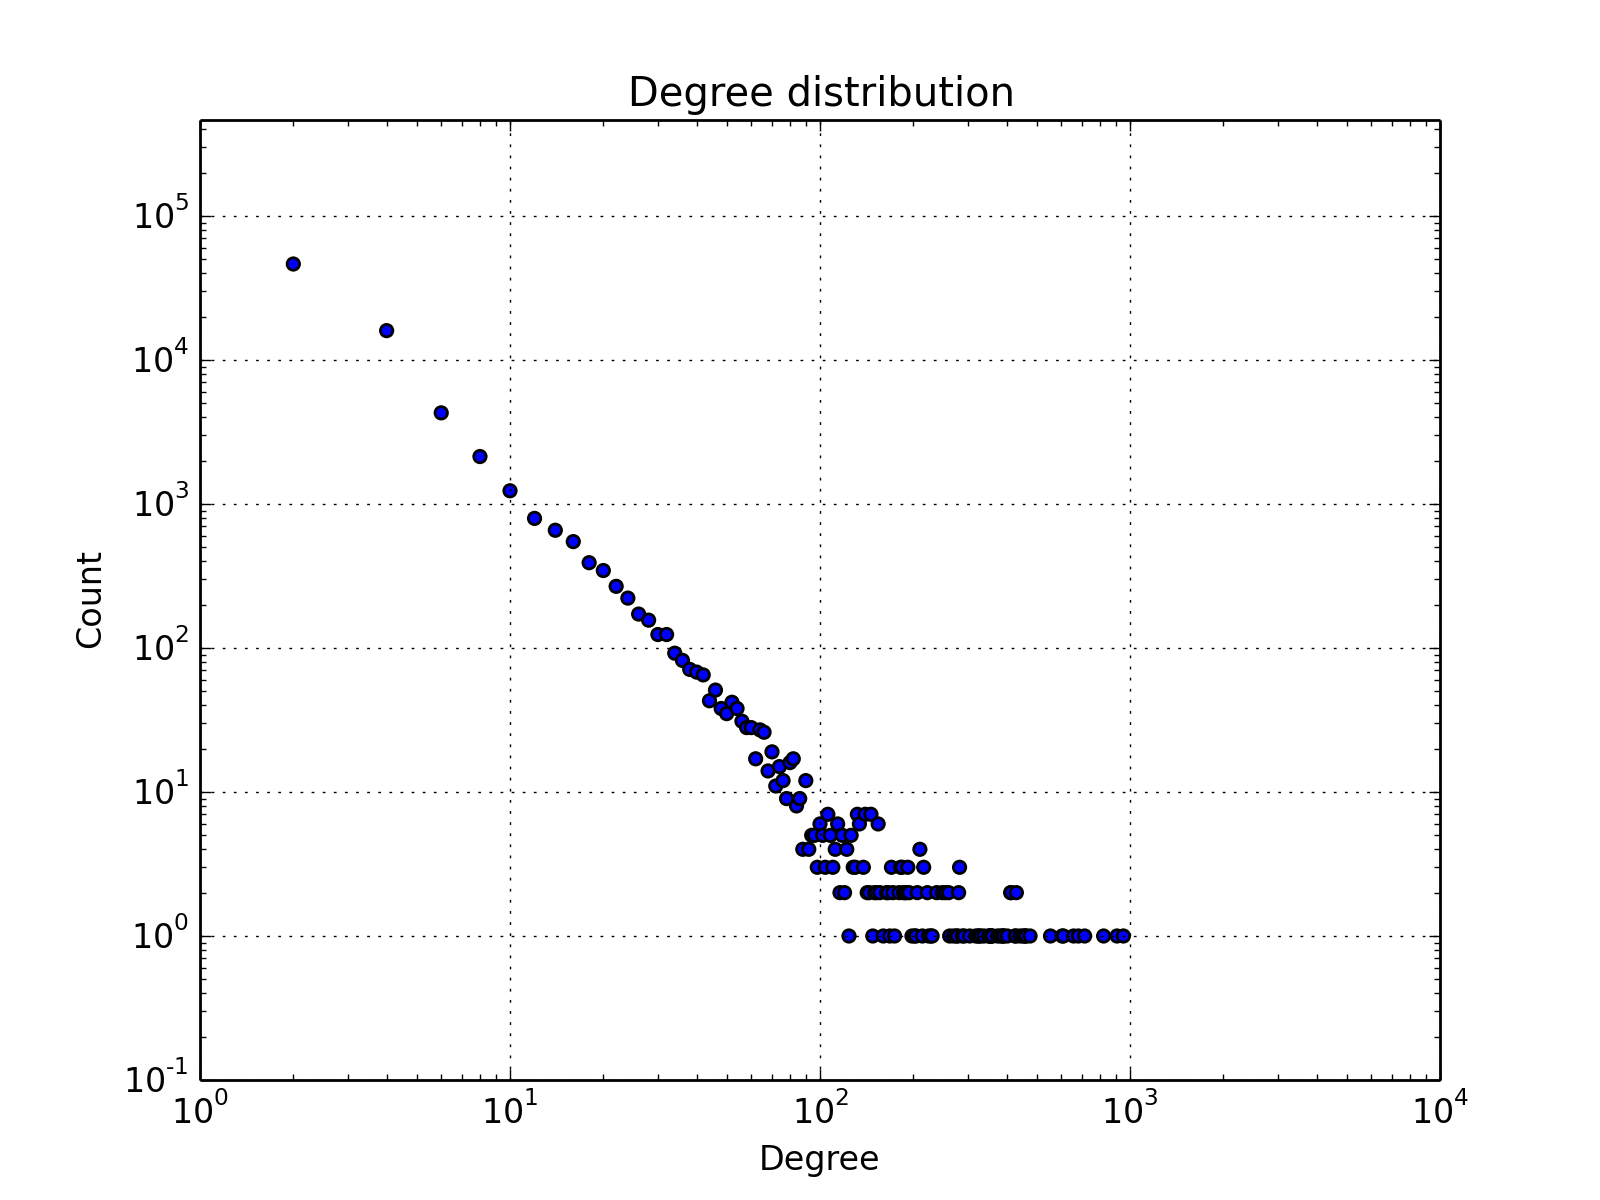
\includegraphics[width=0.35\textwidth]{FIG/DegreeDistoutput_as-skitter.png} 
     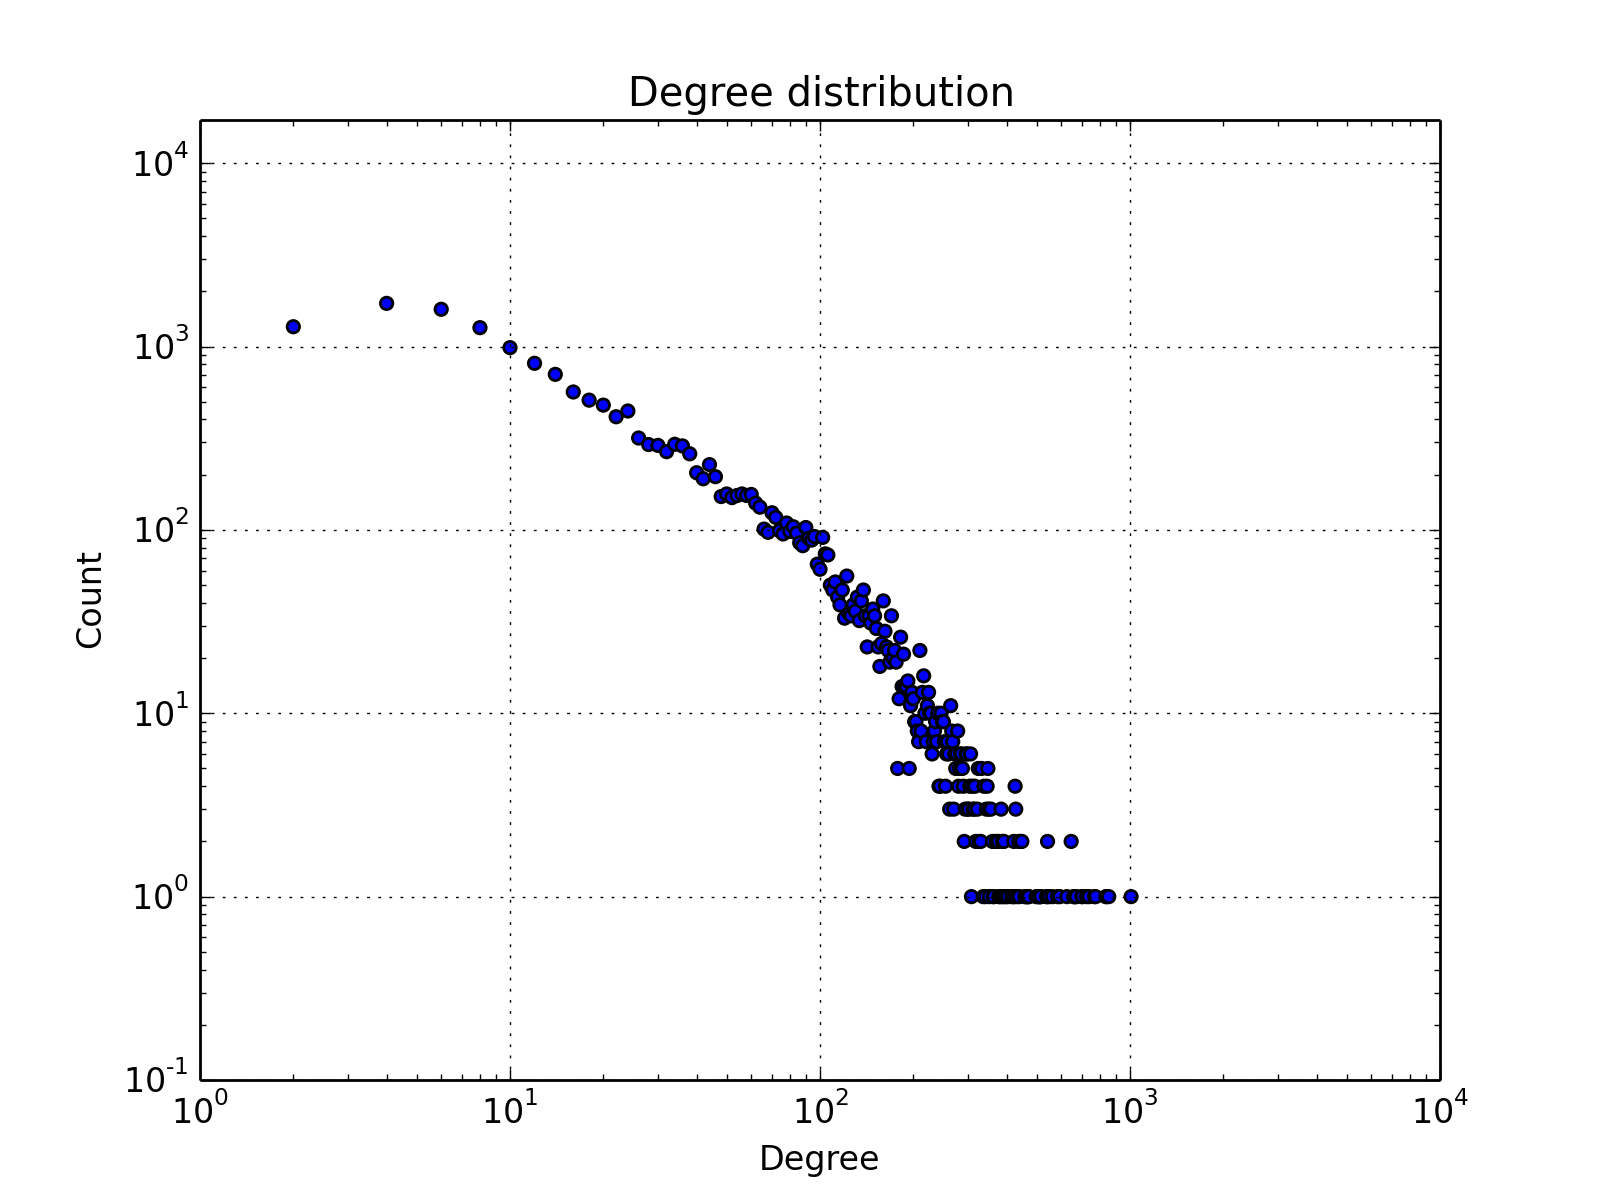
\includegraphics[width=0.35\textwidth]{FIG/DegreeDistoutput_ca-AstroPh.png}
     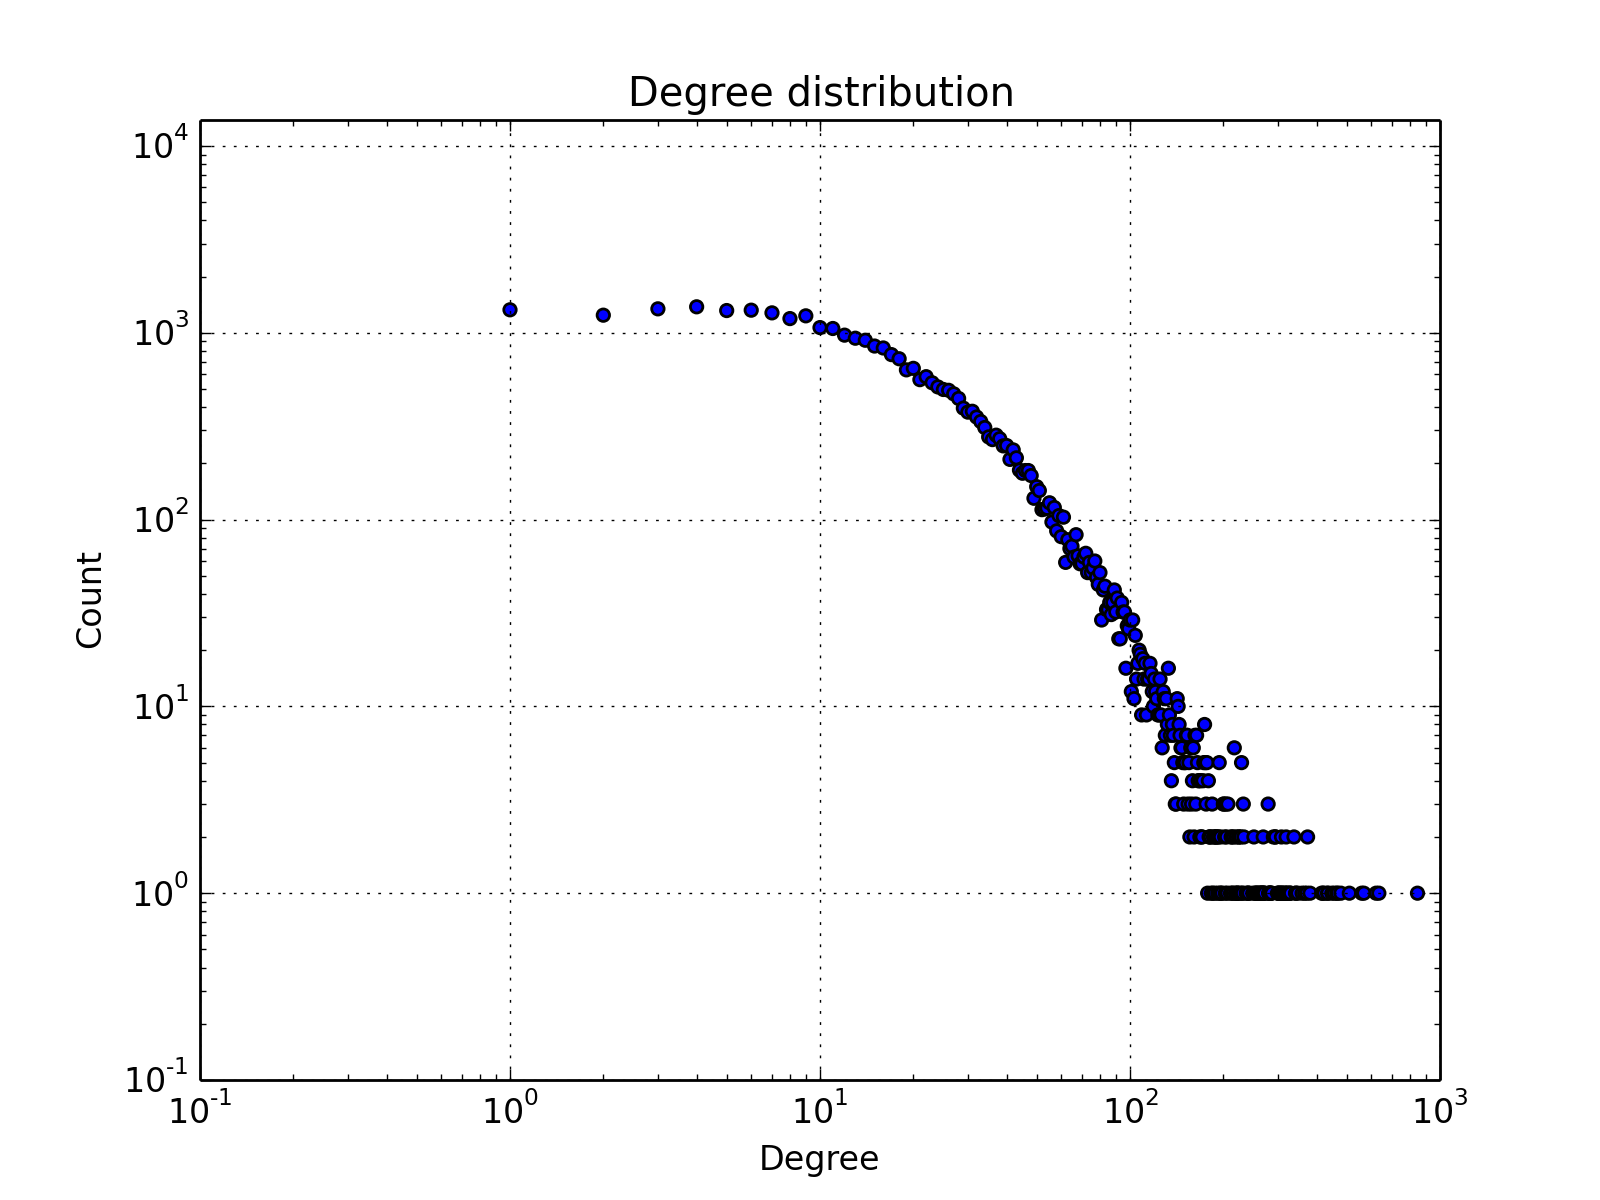
\includegraphics[width=0.35\textwidth]{FIG/DegreeDistoutput_cit-HepPh.png} \\
     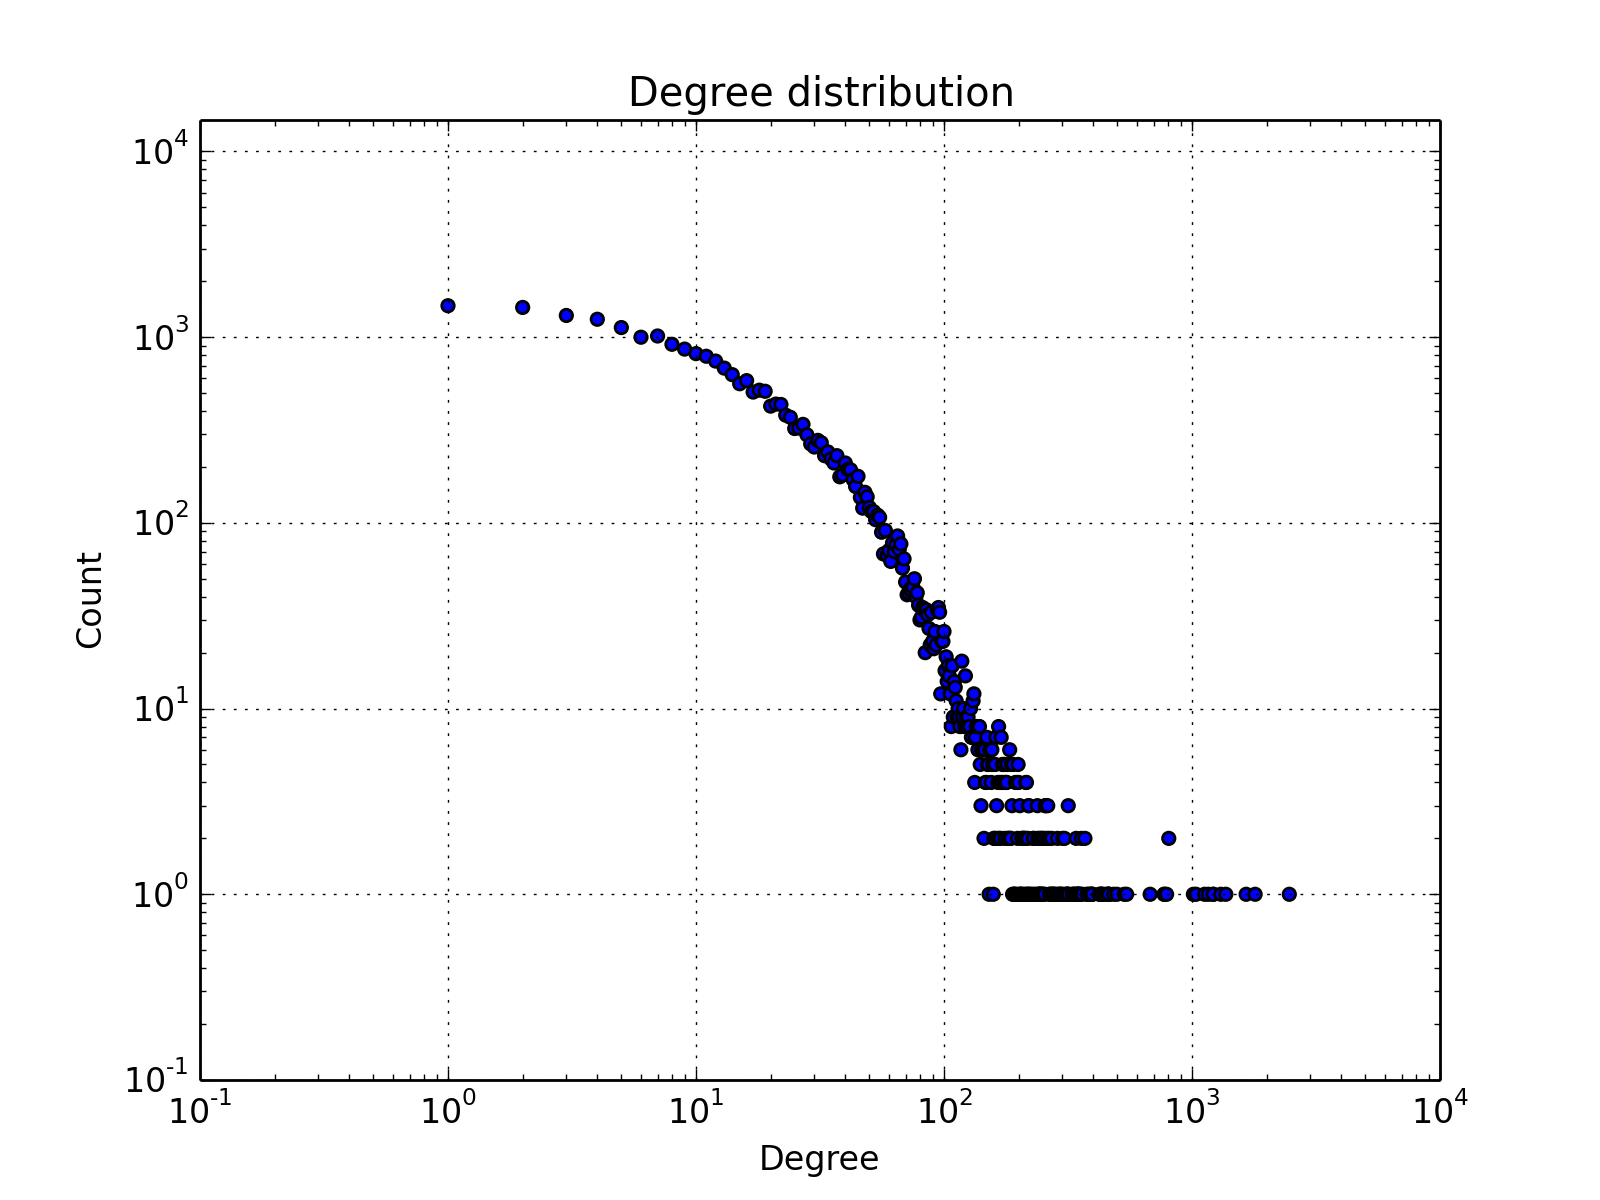
\includegraphics[width=0.35\textwidth]{FIG/DegreeDistoutput_cit-HepTh.png} 
     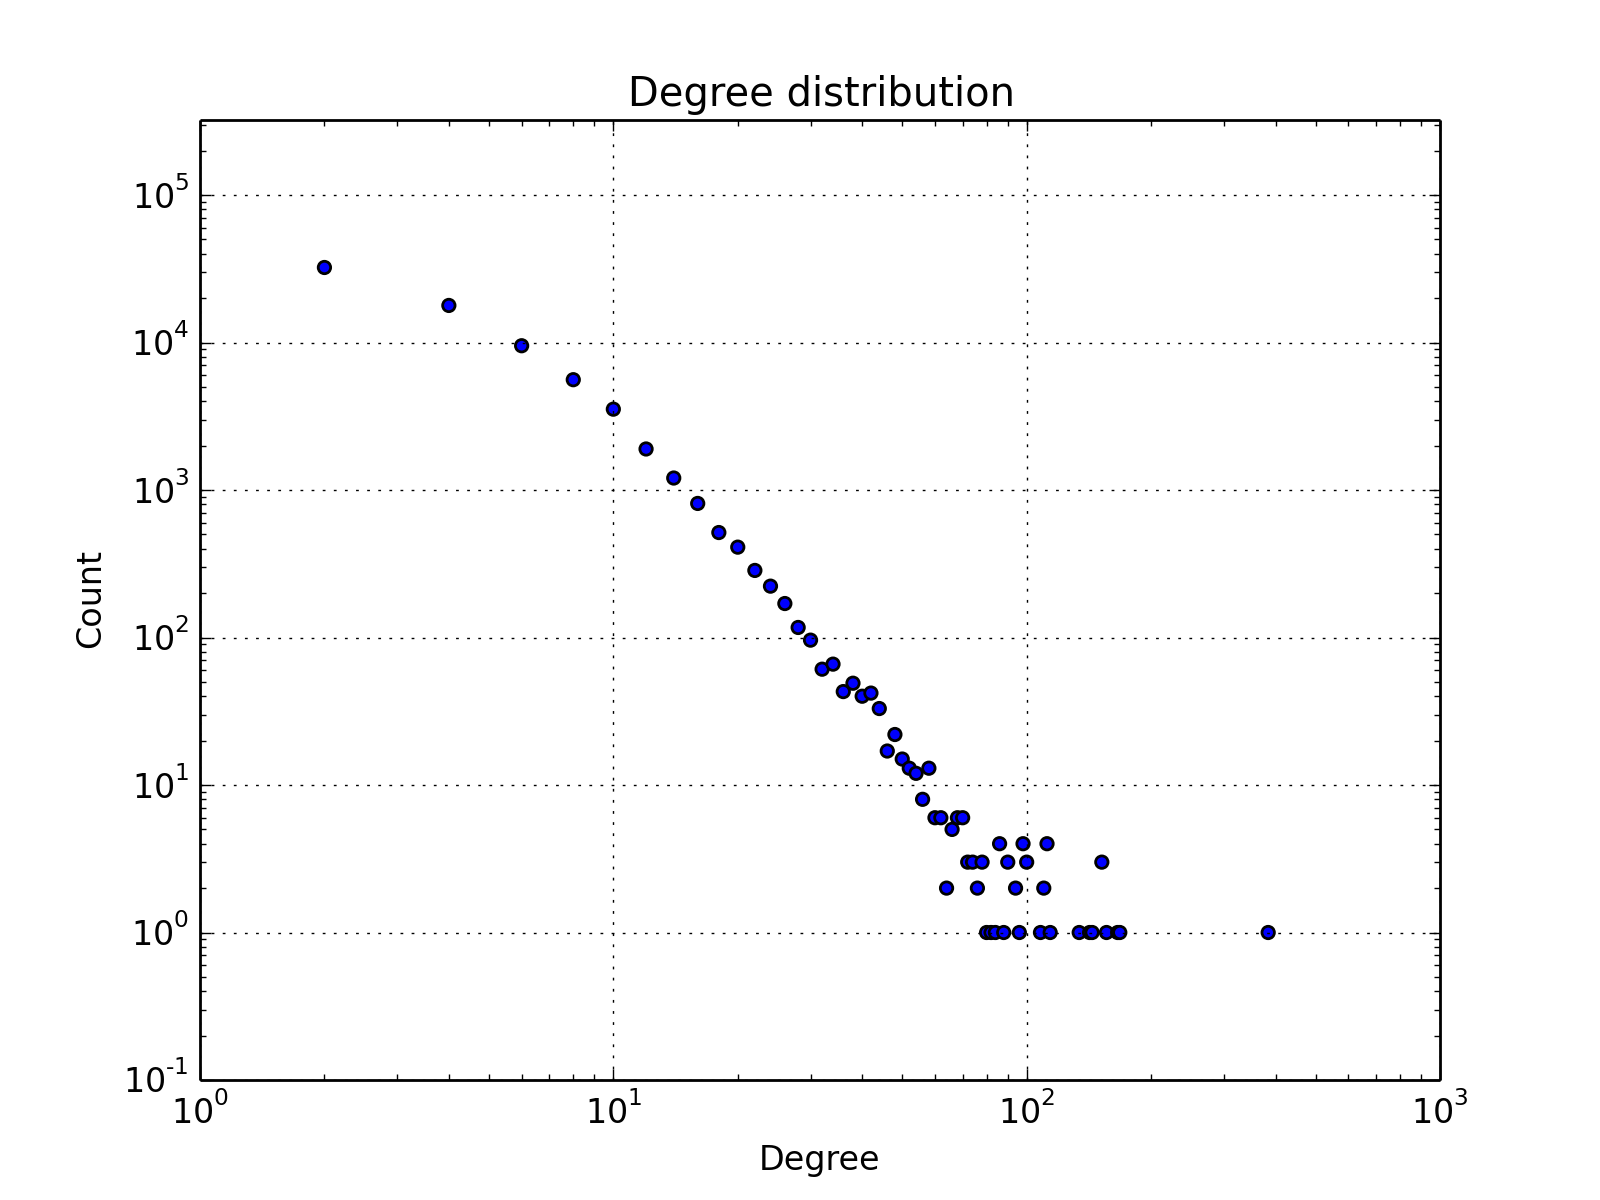
\includegraphics[width=0.35\textwidth]{FIG/DegreeDistoutput_com-amazon.png} 
     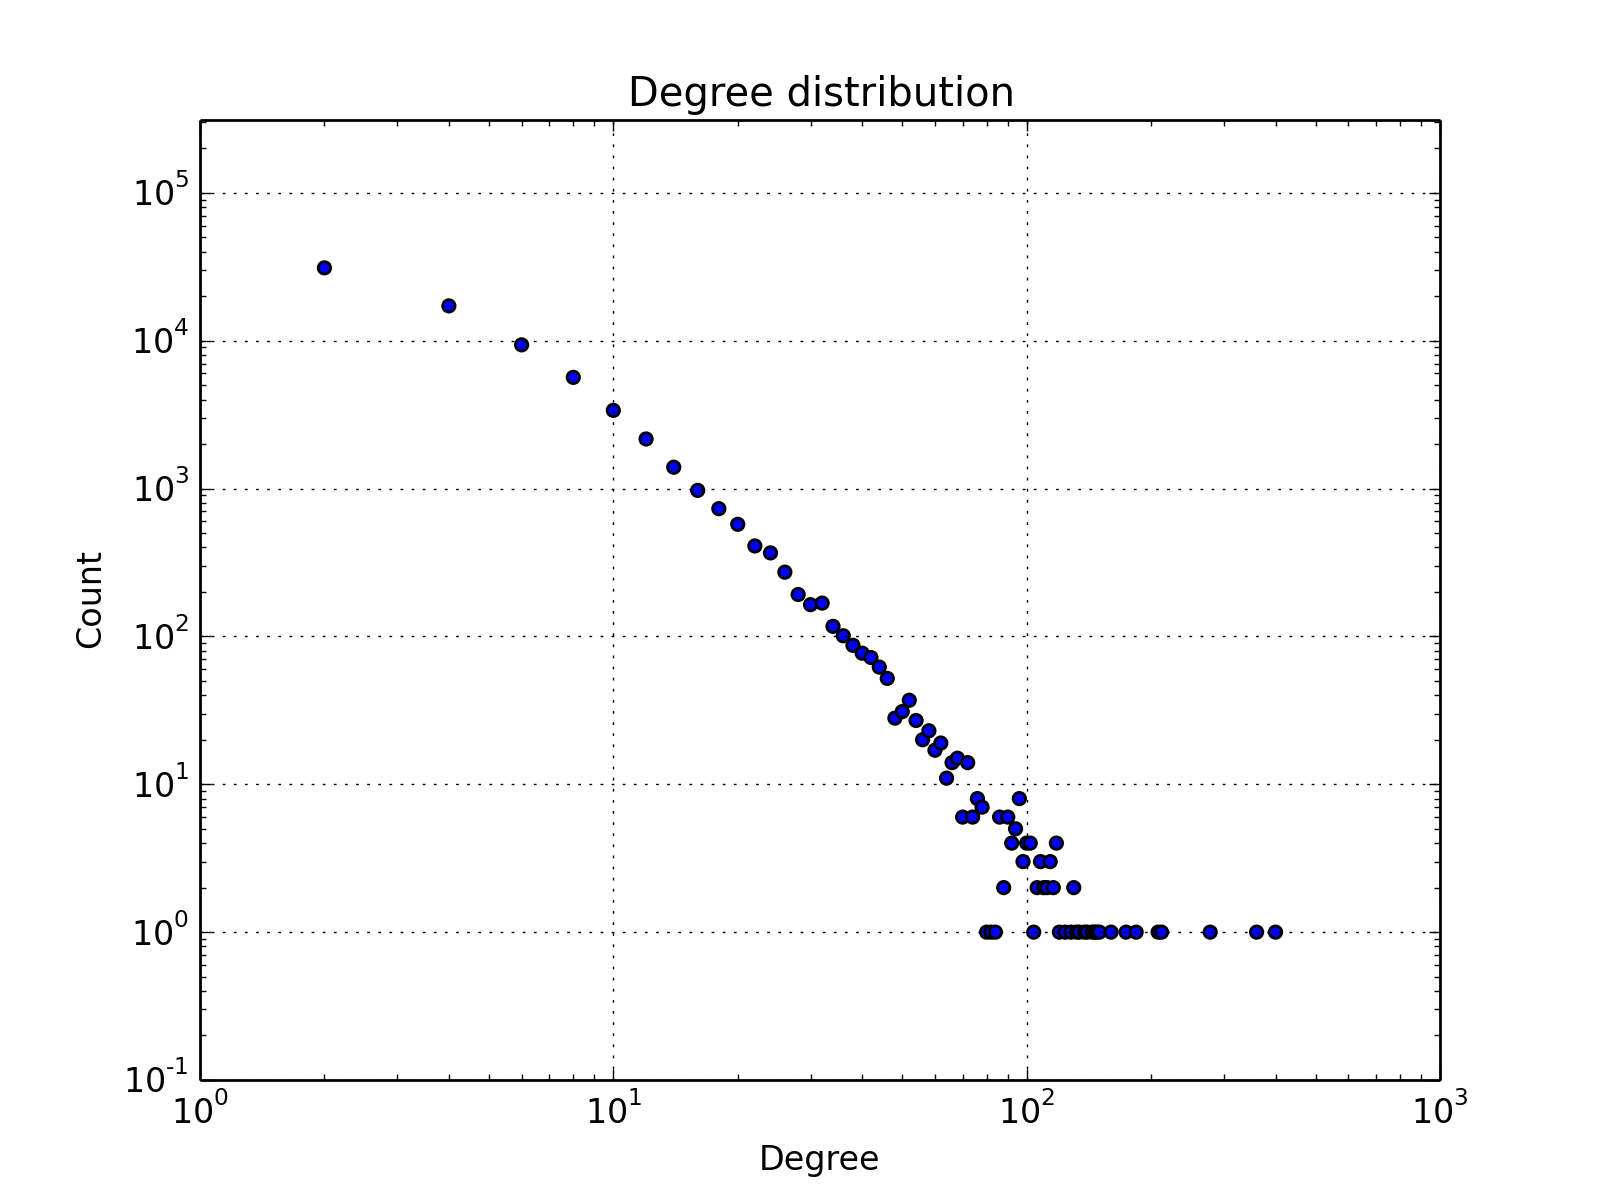
\includegraphics[width=0.35\textwidth]{FIG/DegreeDistoutput_com-dblp.png} \\
     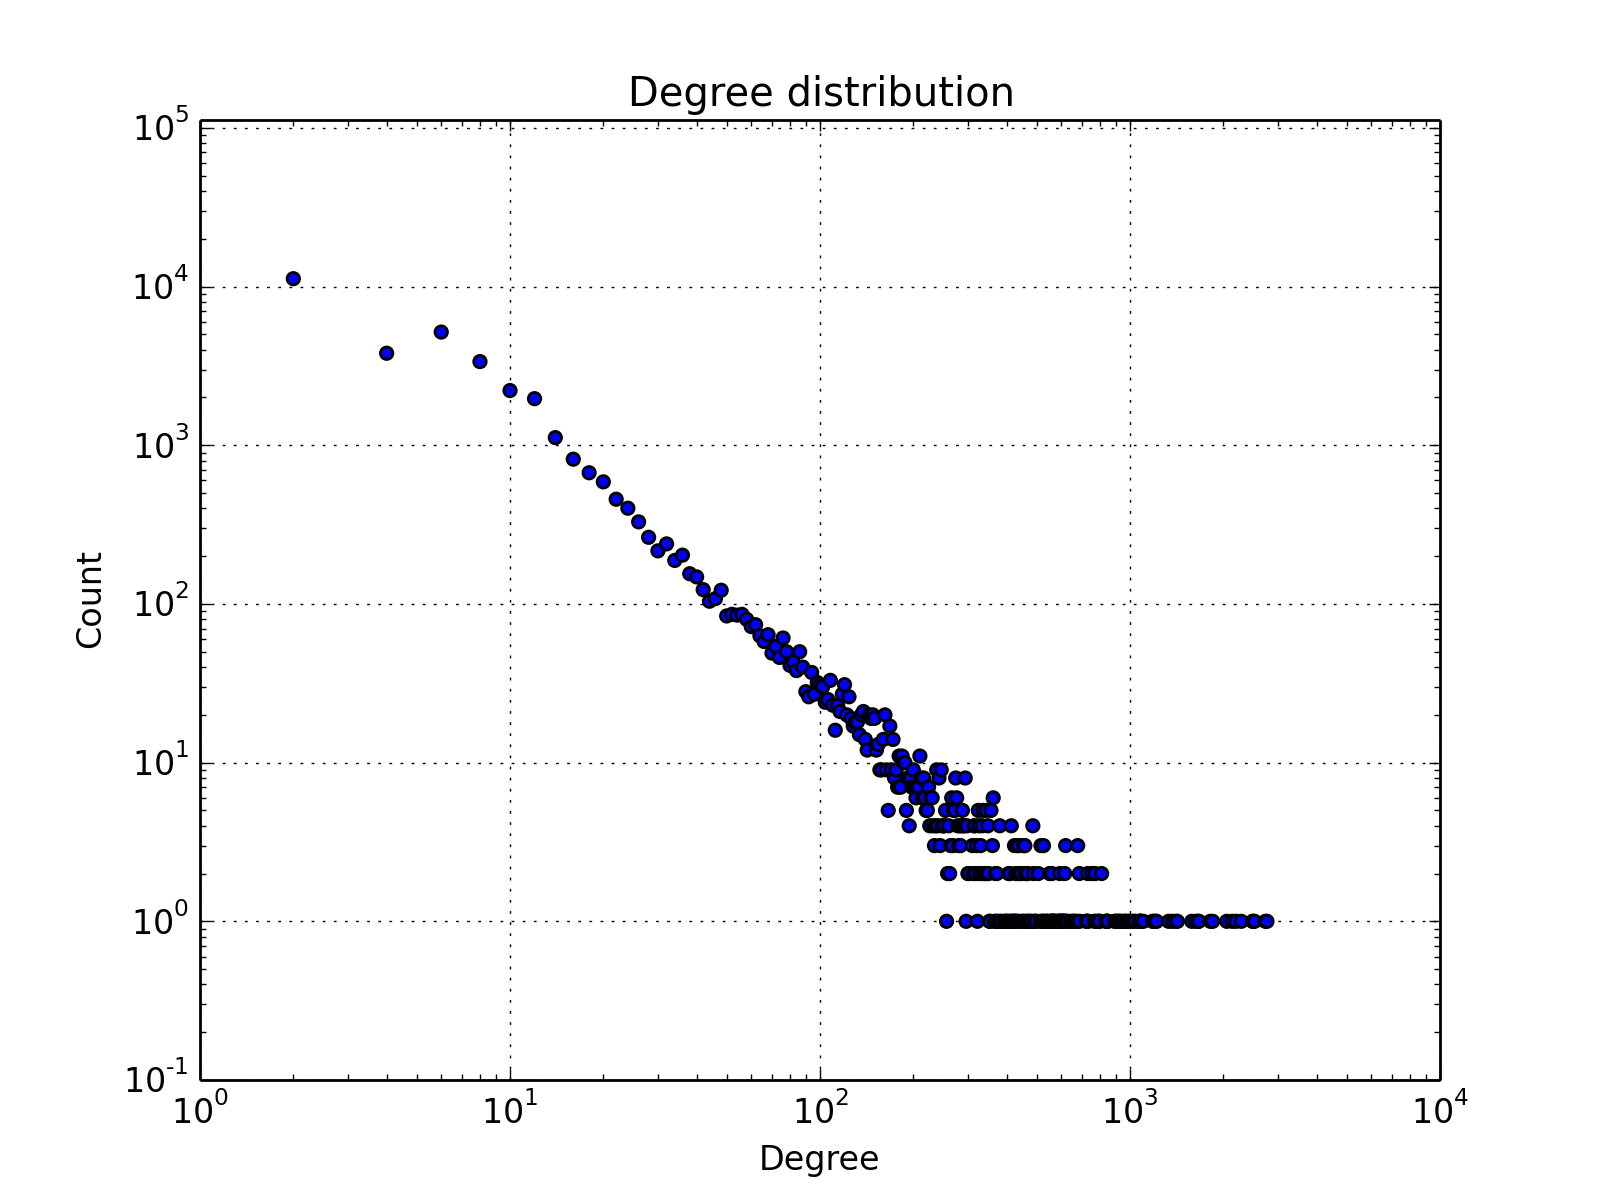
\includegraphics[width=0.35\textwidth]{FIG/DegreeDistoutput_email-Enron.png} 
     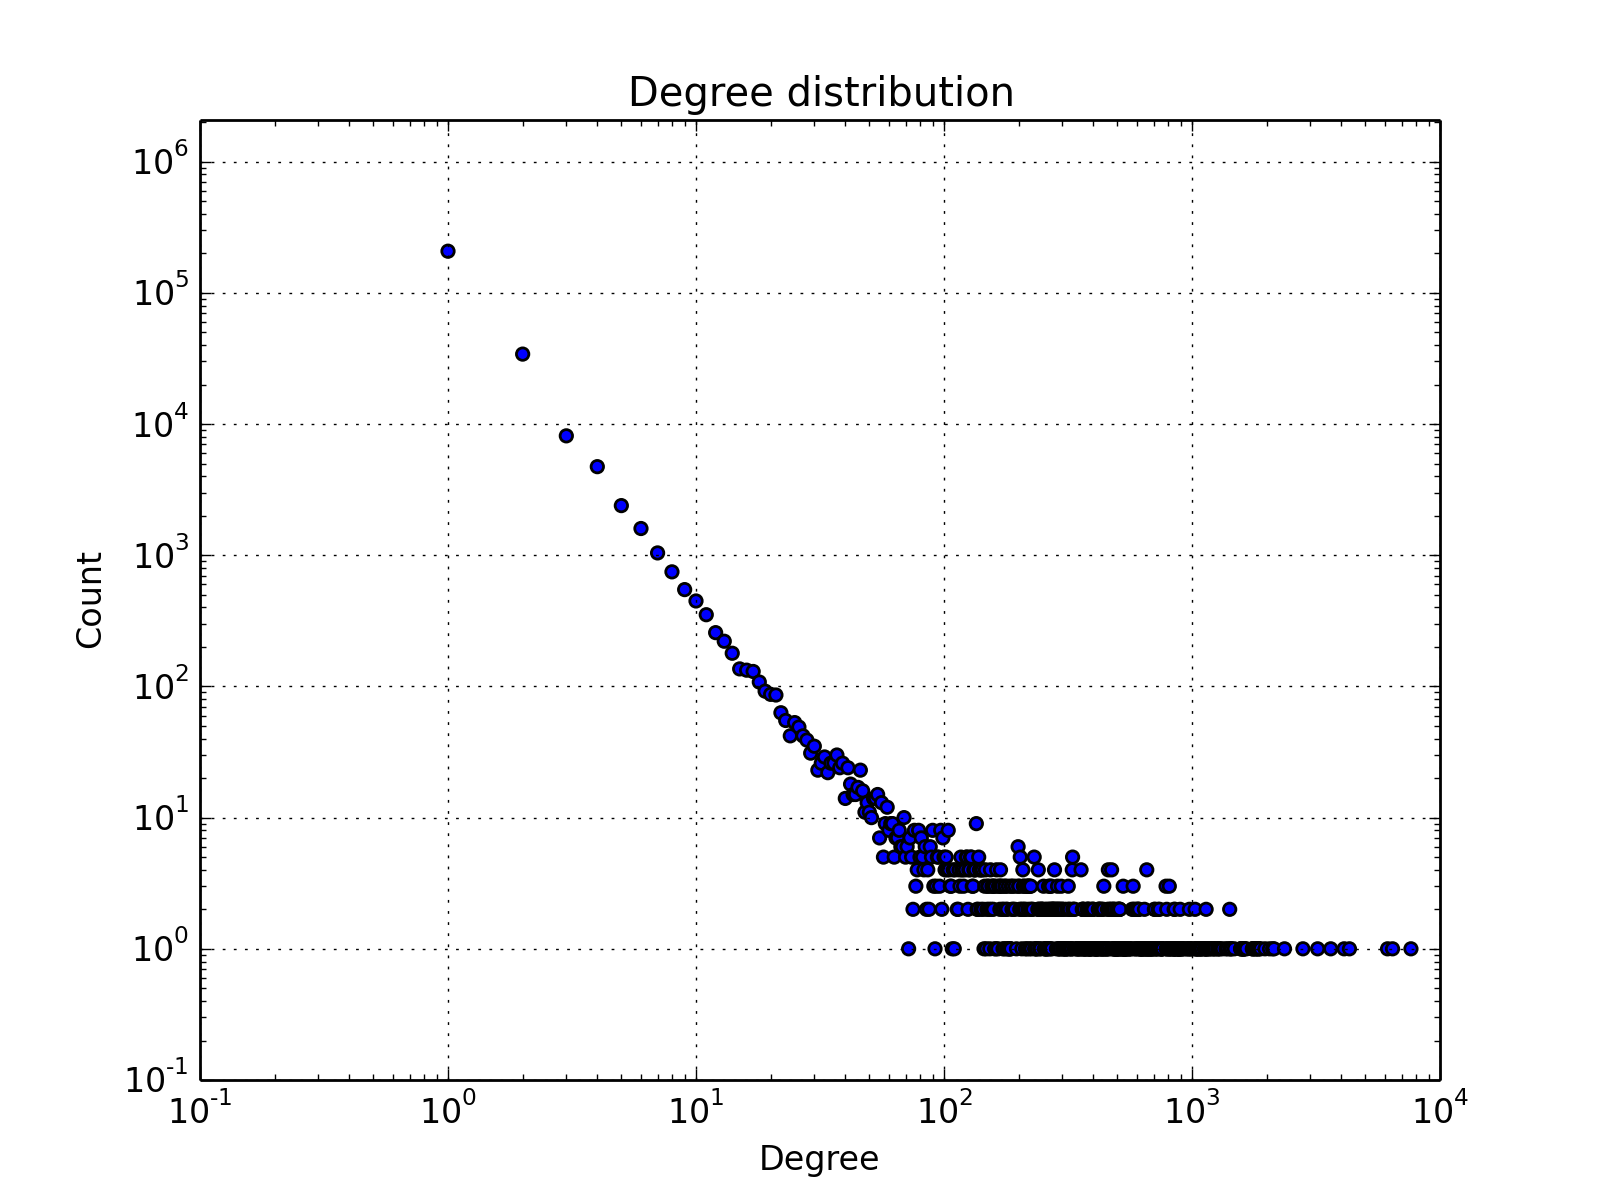
\includegraphics[width=0.35\textwidth]{FIG/DegreeDistoutput_email-EuAll.png} 
     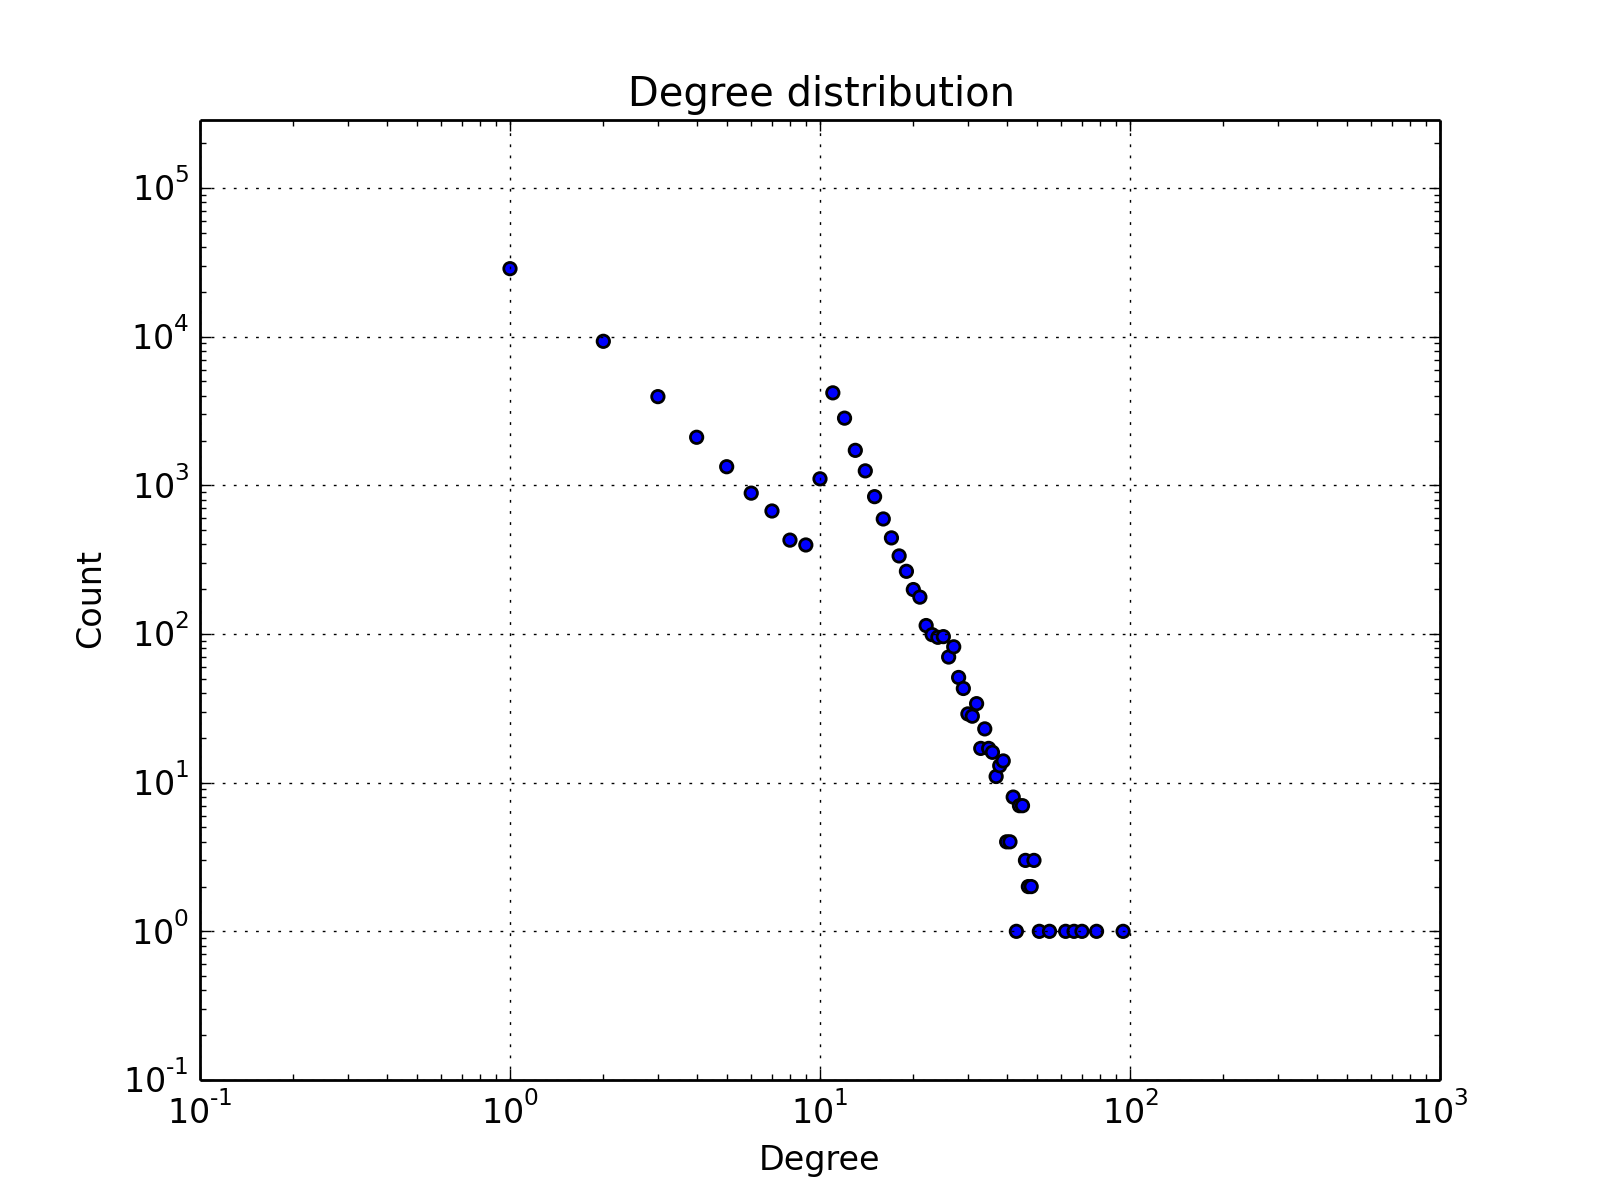
\includegraphics[width=0.35\textwidth]{FIG/DegreeDistoutput_p2p-Gnutella31.png} \\
     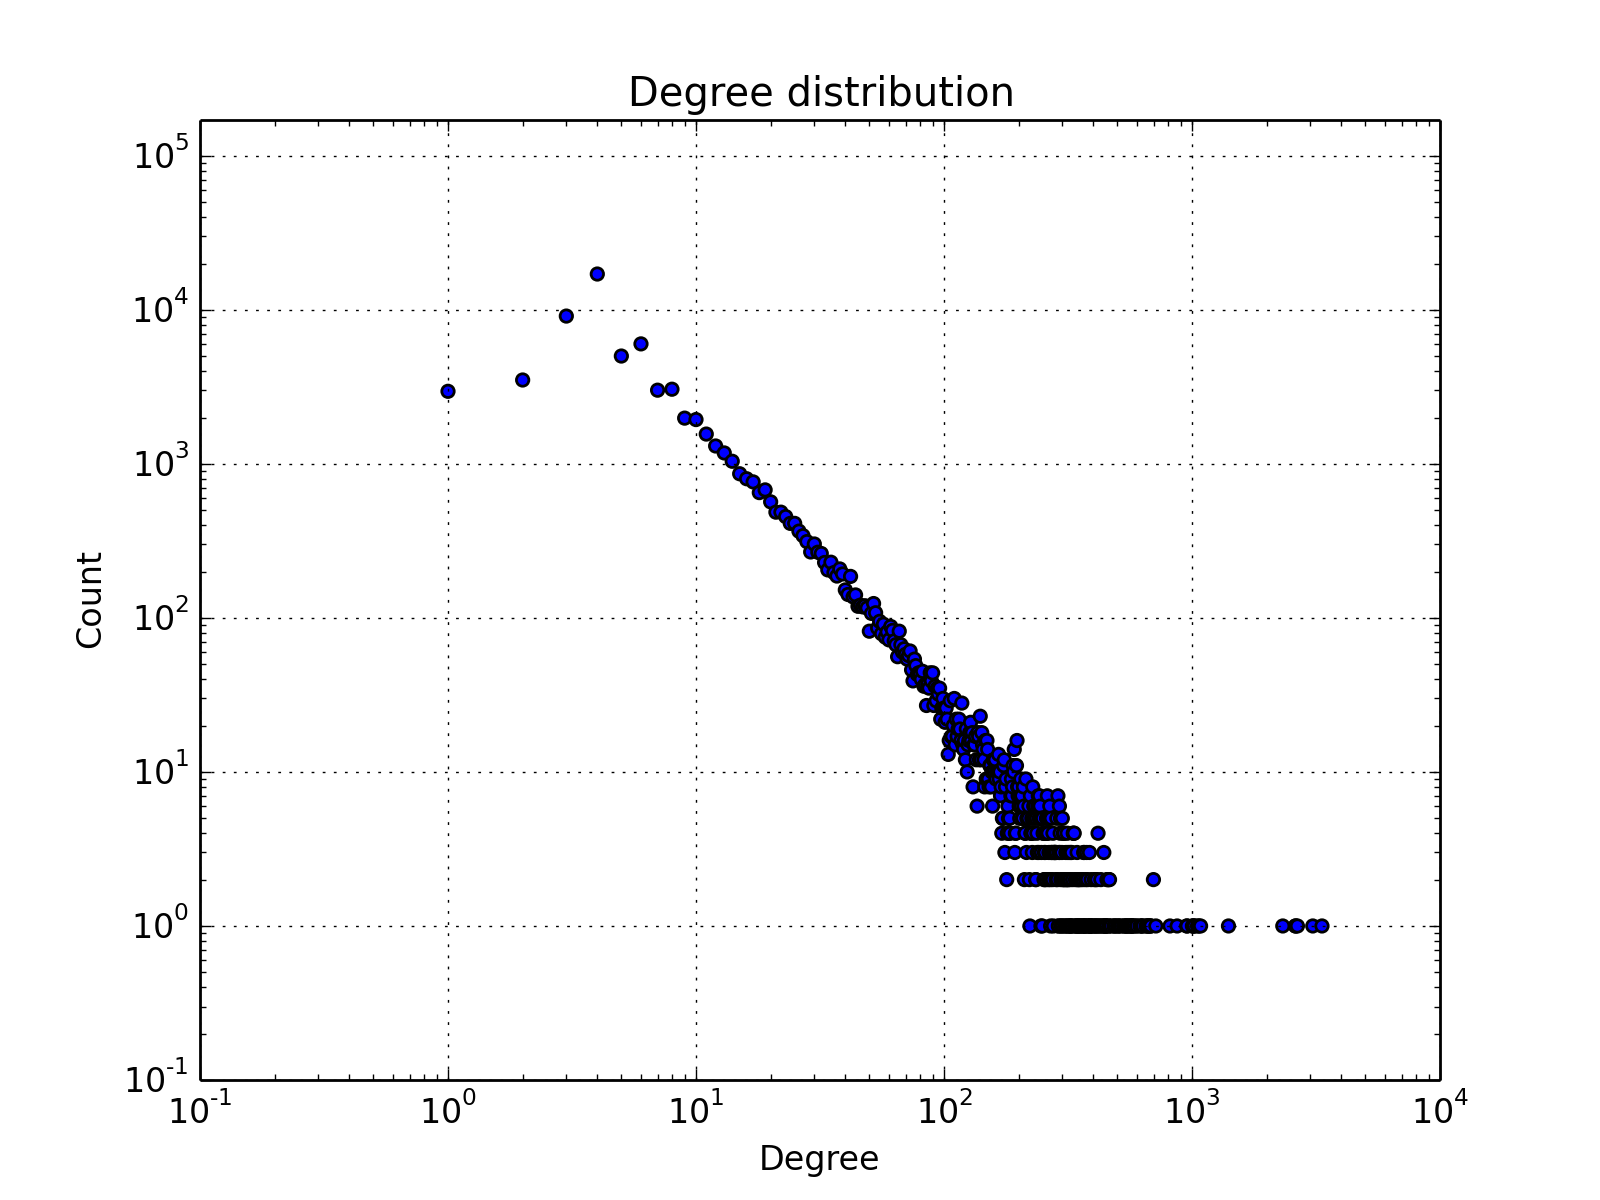
\includegraphics[width=0.35\textwidth]{FIG/DegreeDistoutput_soc-Slashdot0811-75000.png} 
\end{tabular}
\caption{Degree distribution plots of 10 graphs}
\label{fig:results}
\end{center}
\end{figure}

For 6 directed graphs out of all 10 graphs, we can also plot Indegree vs. Count and Outdegree vs. Count in log space

\begin{figure}[H]
\begin{center}
\begin{tabular}{ccc}
     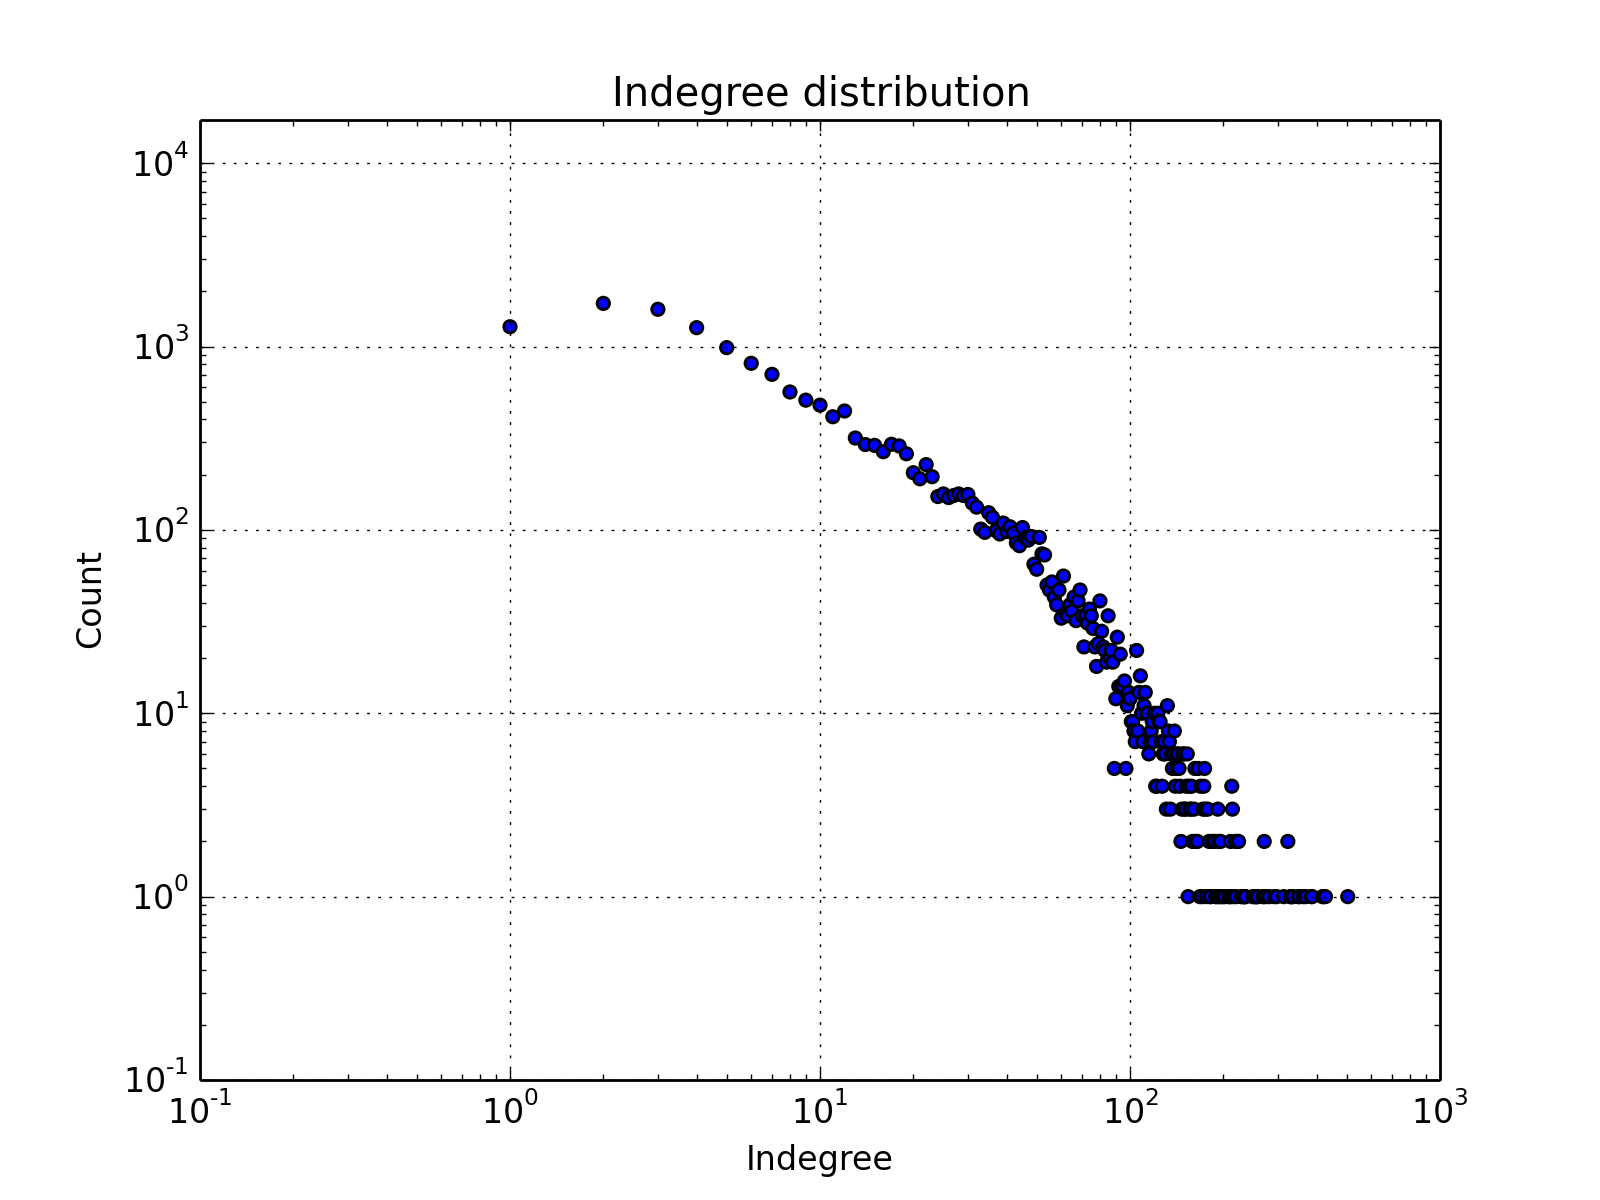
\includegraphics[width=0.35\textwidth]{FIG/IndegreeDistoutput_ca-AstroPh.png}
     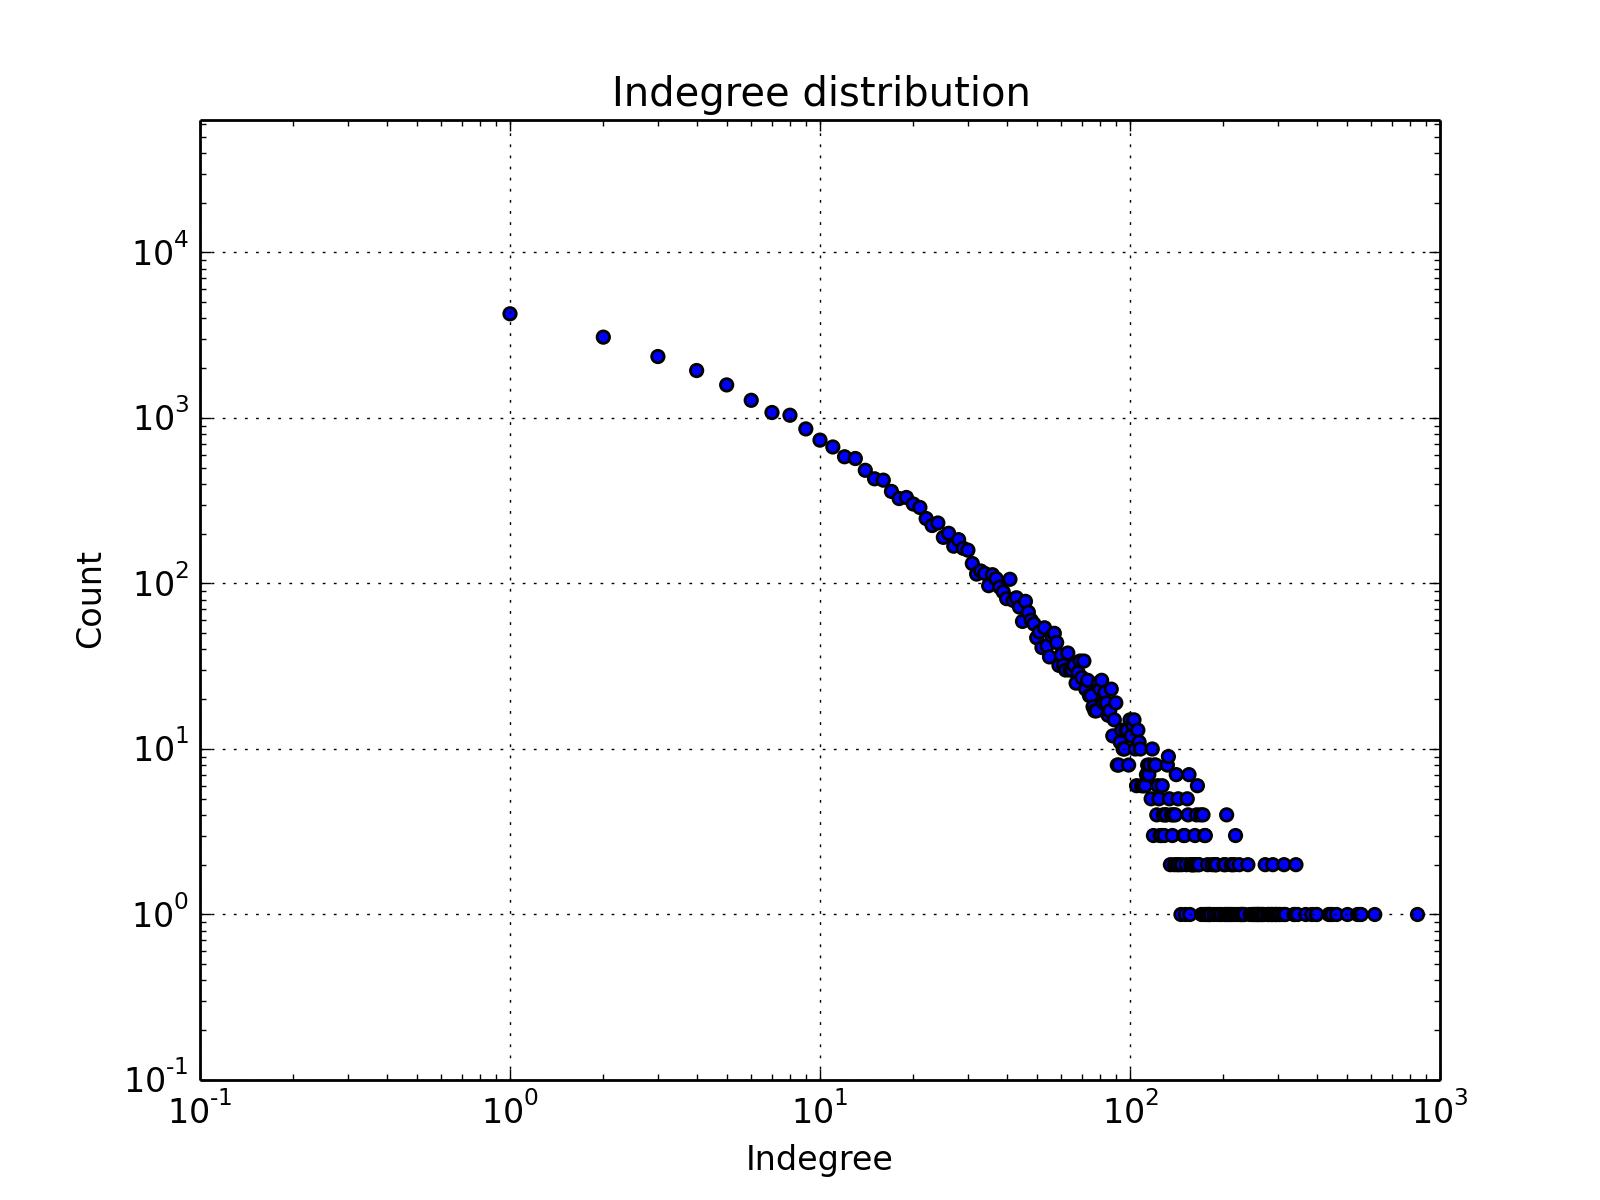
\includegraphics[width=0.35\textwidth]{FIG/IndegreeDistoutput_cit-HepPh.png} 
     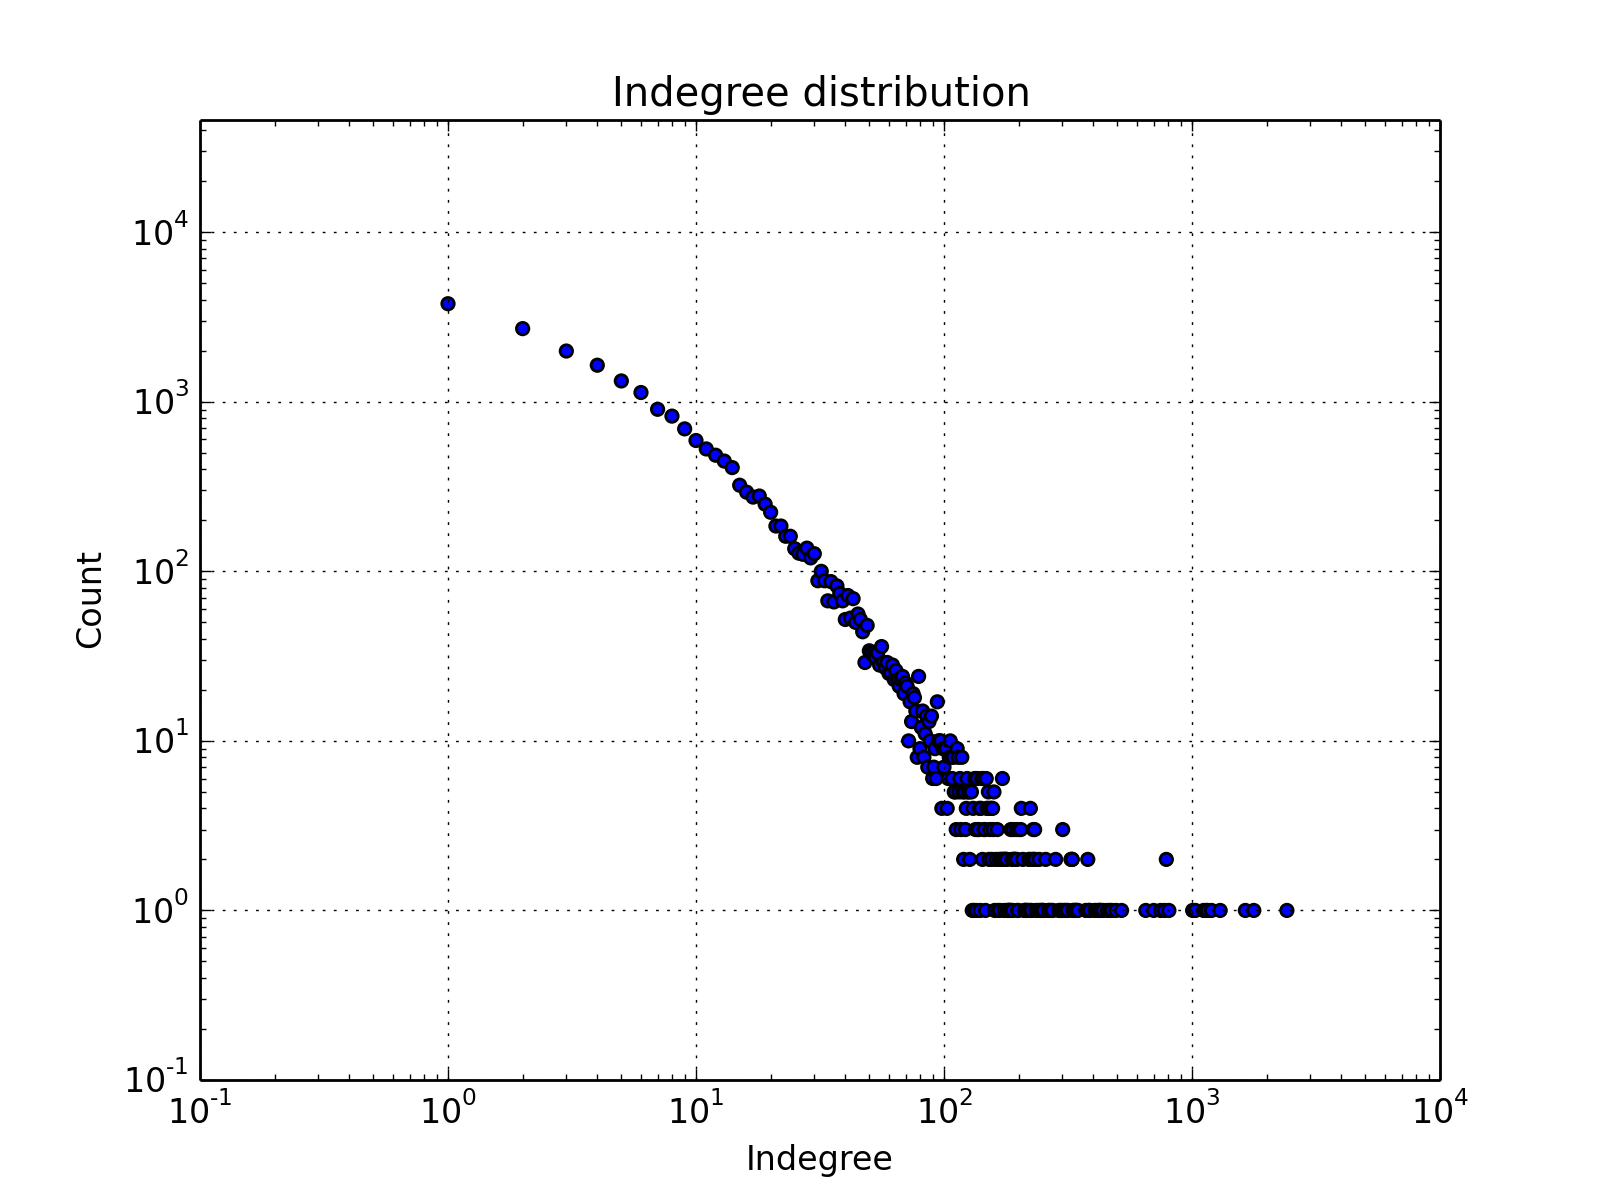
\includegraphics[width=0.35\textwidth]{FIG/IndegreeDistoutput_cit-HepTh.png} \\
     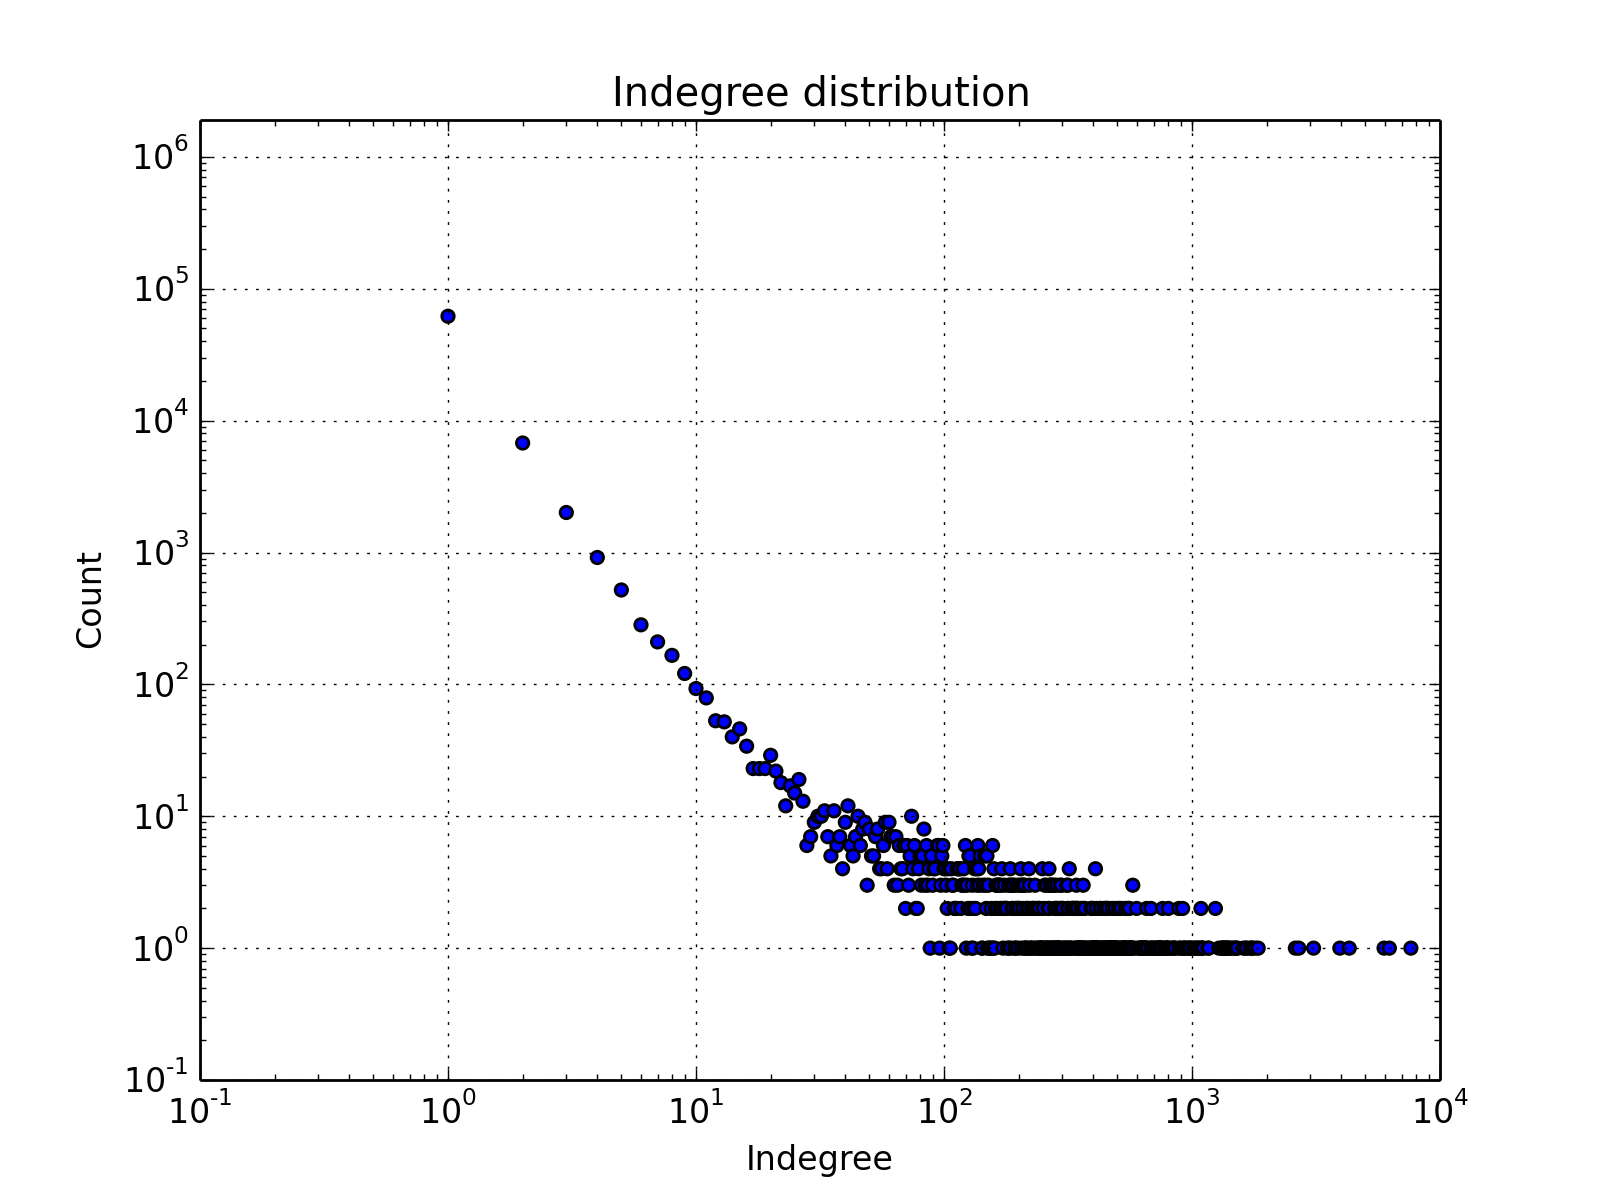
\includegraphics[width=0.35\textwidth]{FIG/IndegreeDistoutput_email-EuAll.png} 
     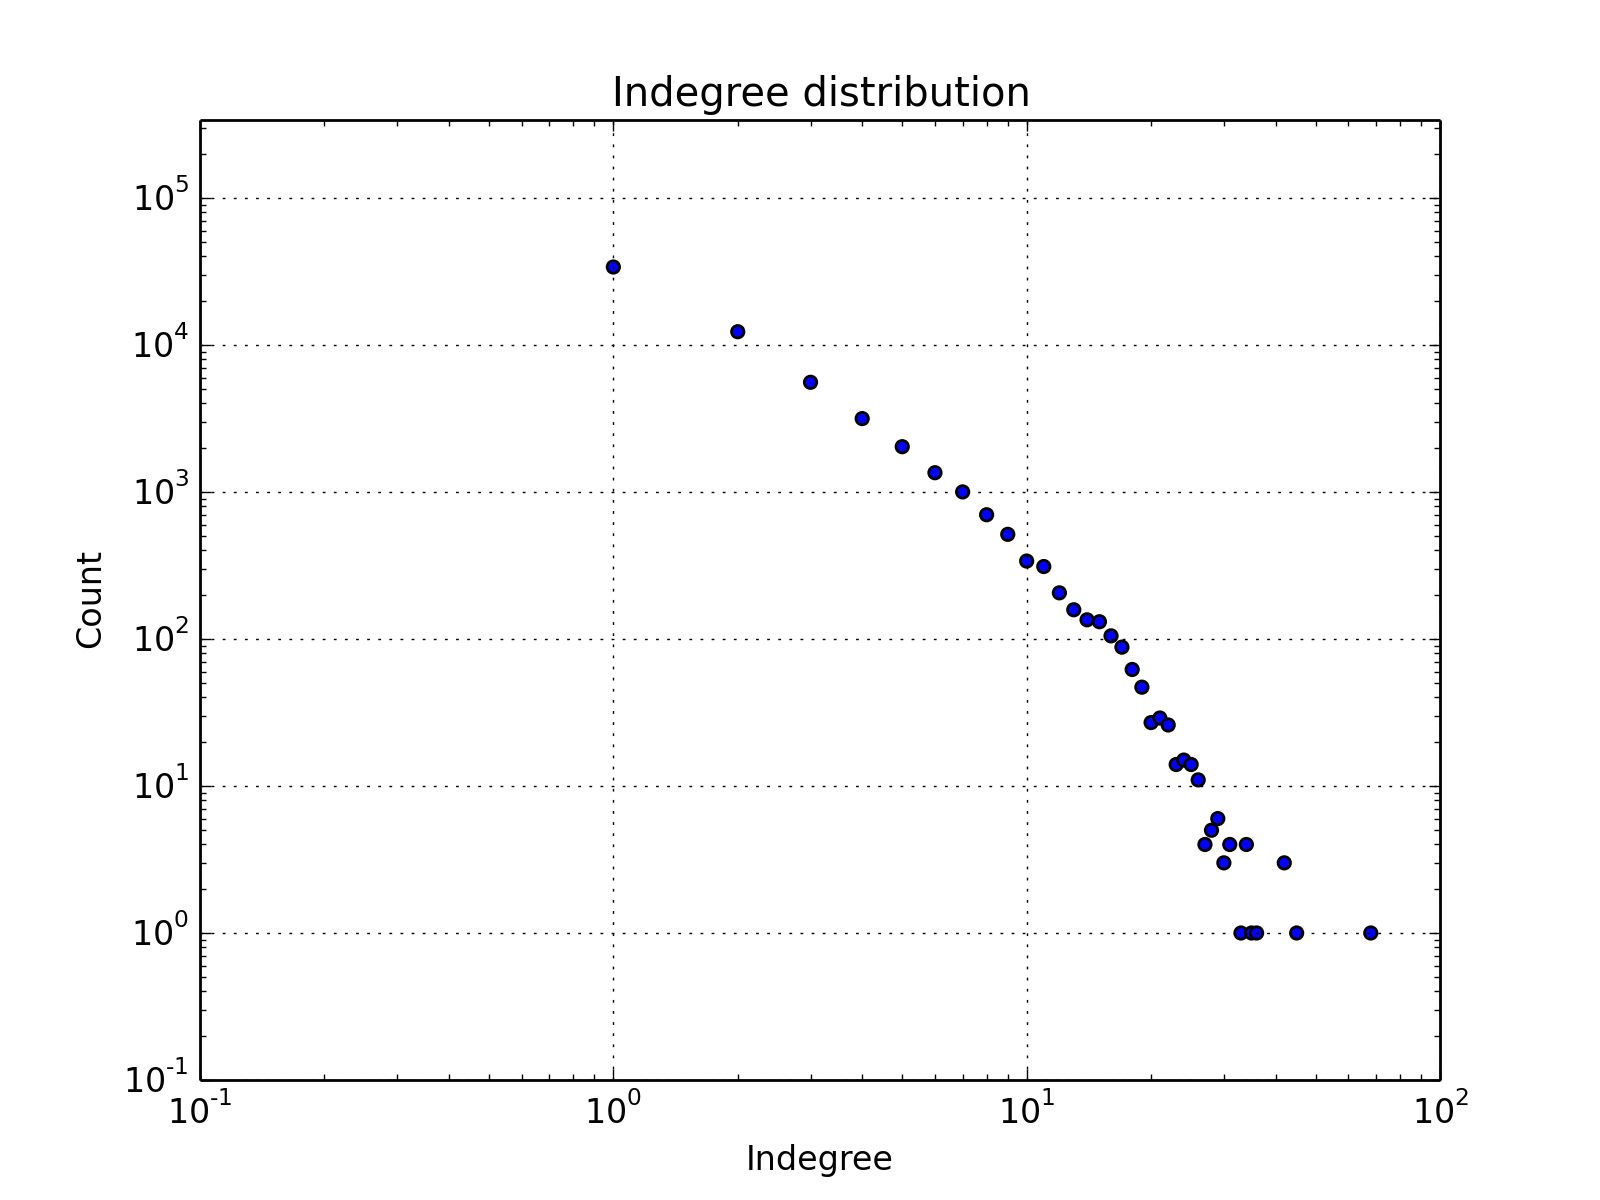
\includegraphics[width=0.35\textwidth]{FIG/IndegreeDistoutput_p2p-Gnutella31.png} 
     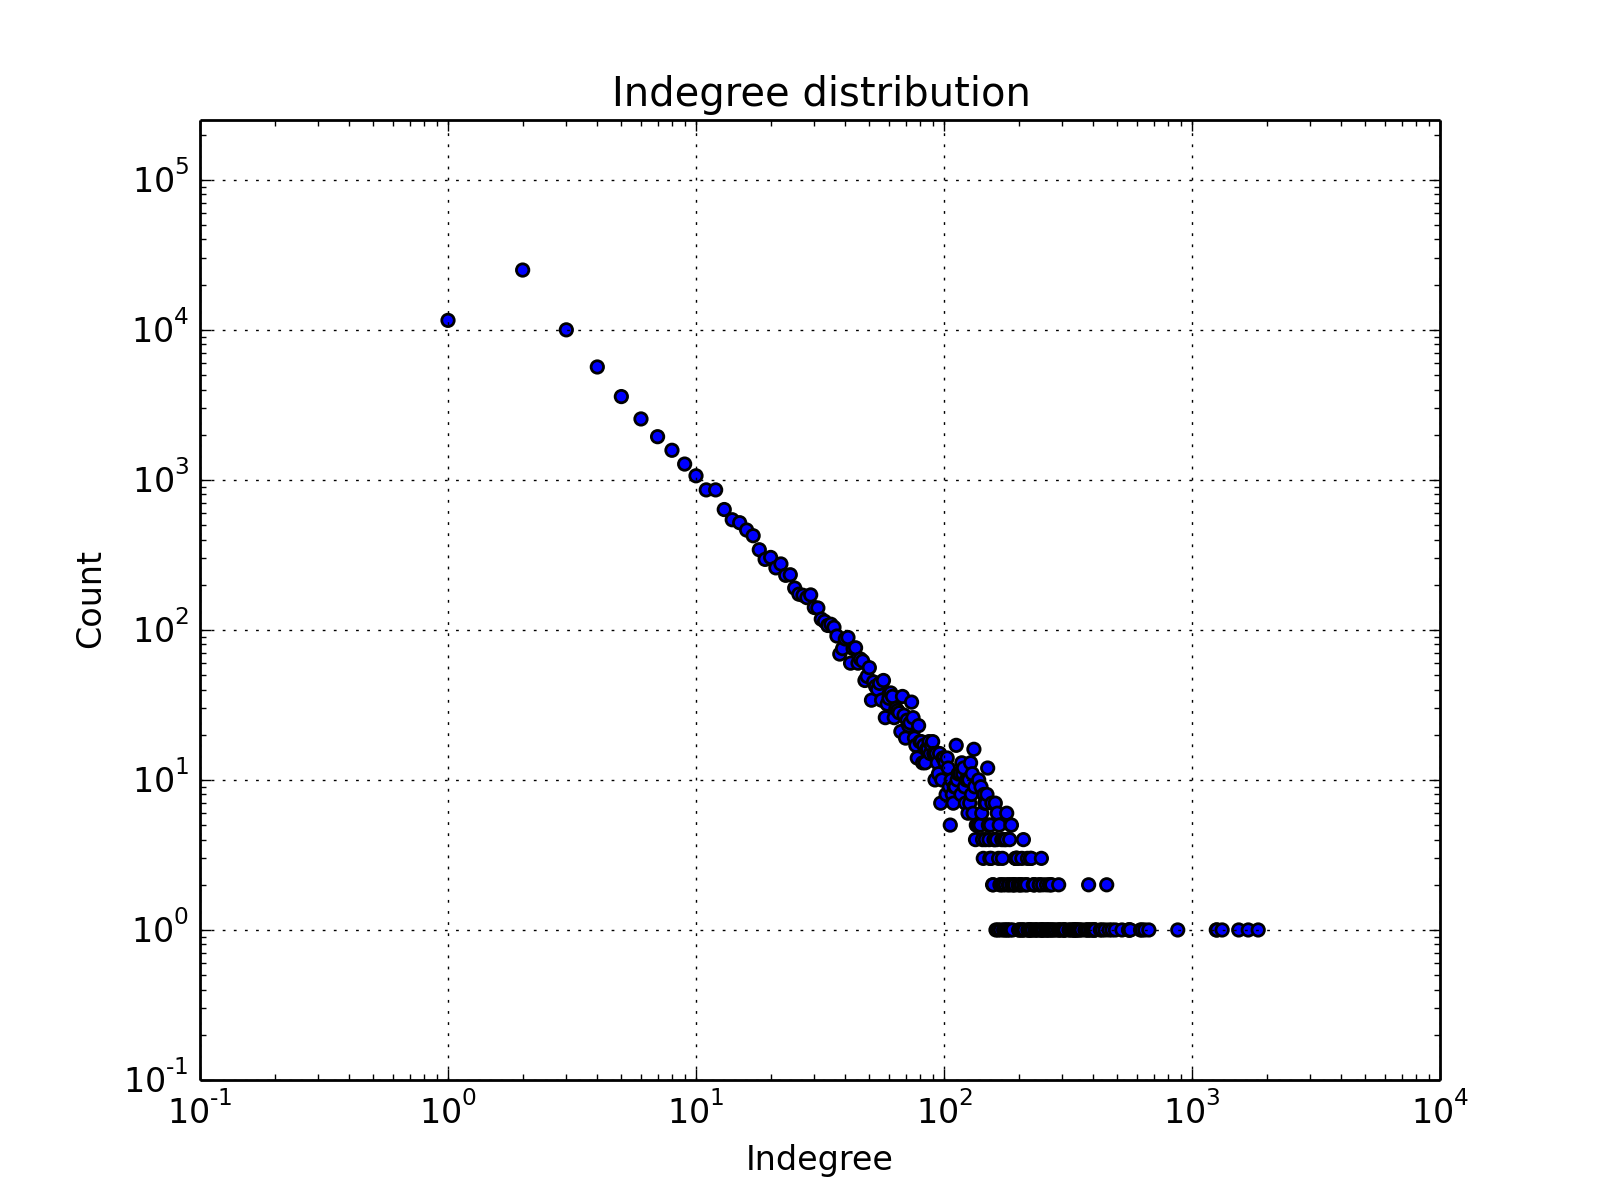
\includegraphics[width=0.35\textwidth]{FIG/IndegreeDistoutput_soc-Slashdot0811-75000.png} 
\end{tabular}
\caption{Indegree distribution plots of 6 directed graphs}
\label{fig:results}
\end{center}
\end{figure}

\begin{figure}[H]
\begin{center}
\begin{tabular}{ccc}
     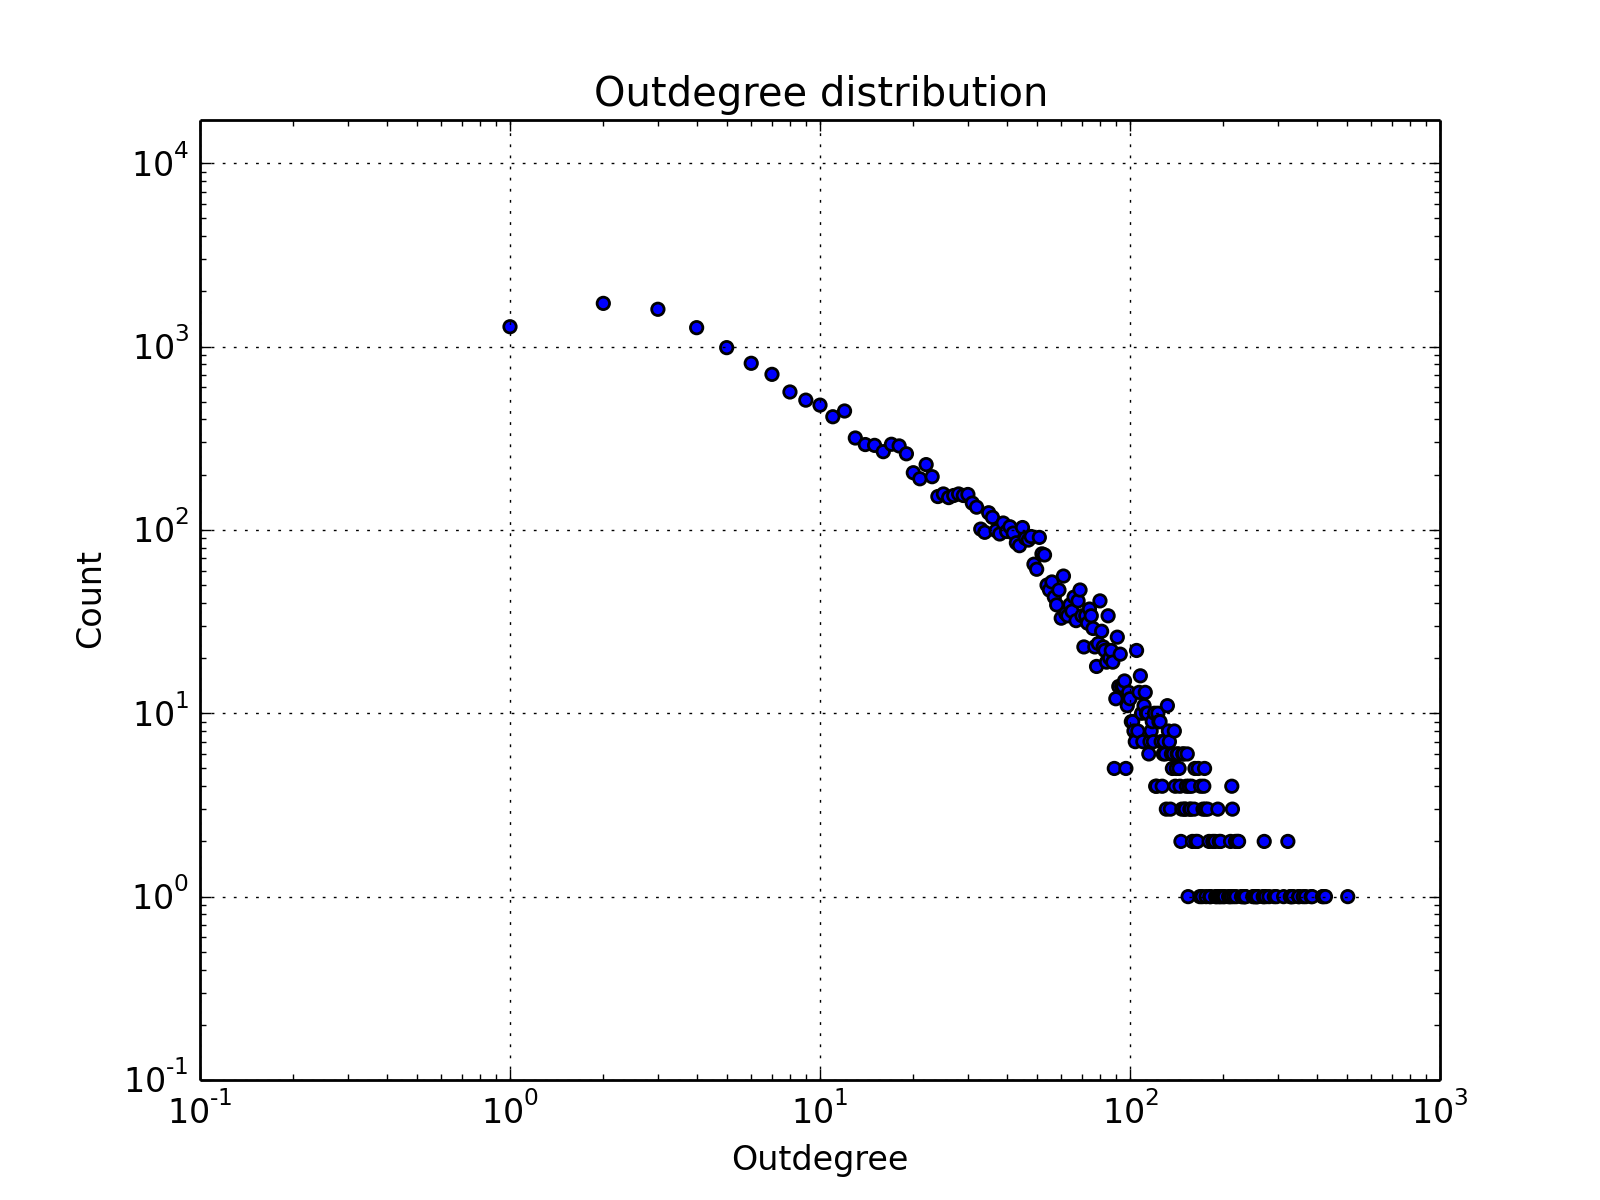
\includegraphics[width=0.35\textwidth]{FIG/OutdegreeDistoutput_ca-AstroPh.png}
     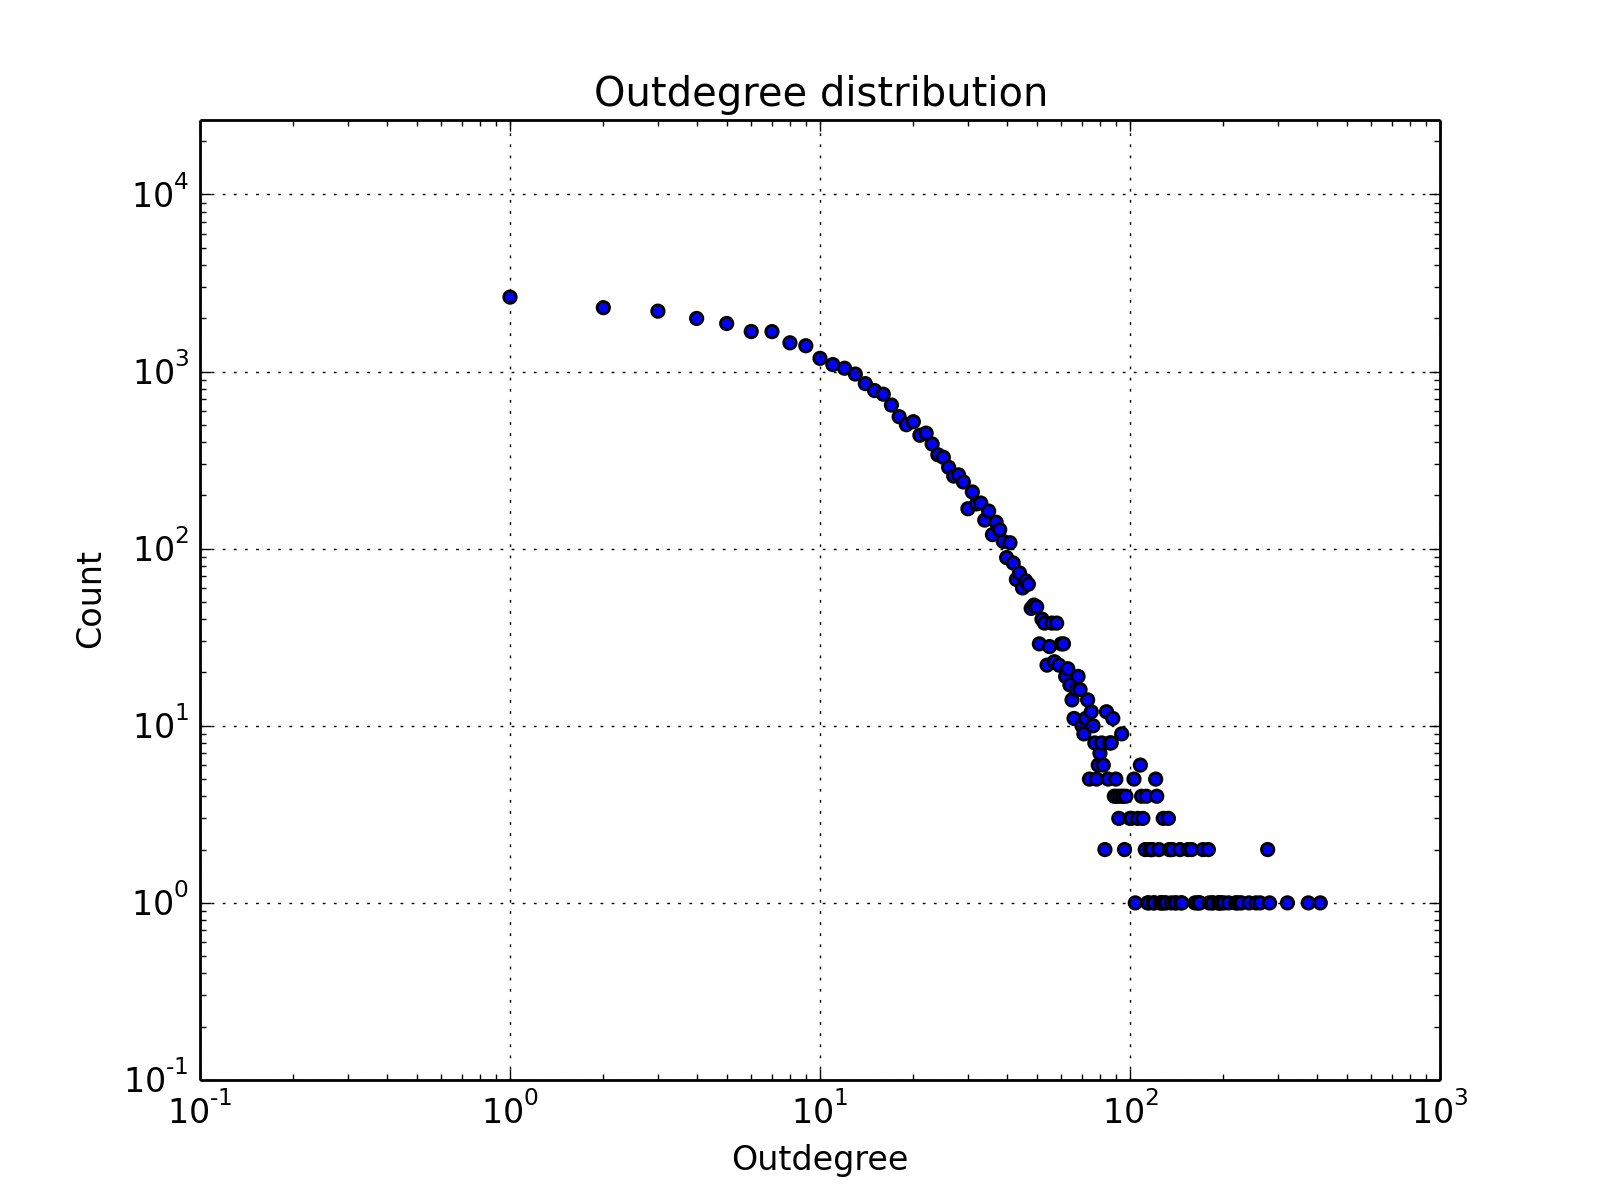
\includegraphics[width=0.35\textwidth]{FIG/OutdegreeDistoutput_cit-HepPh.png} 
     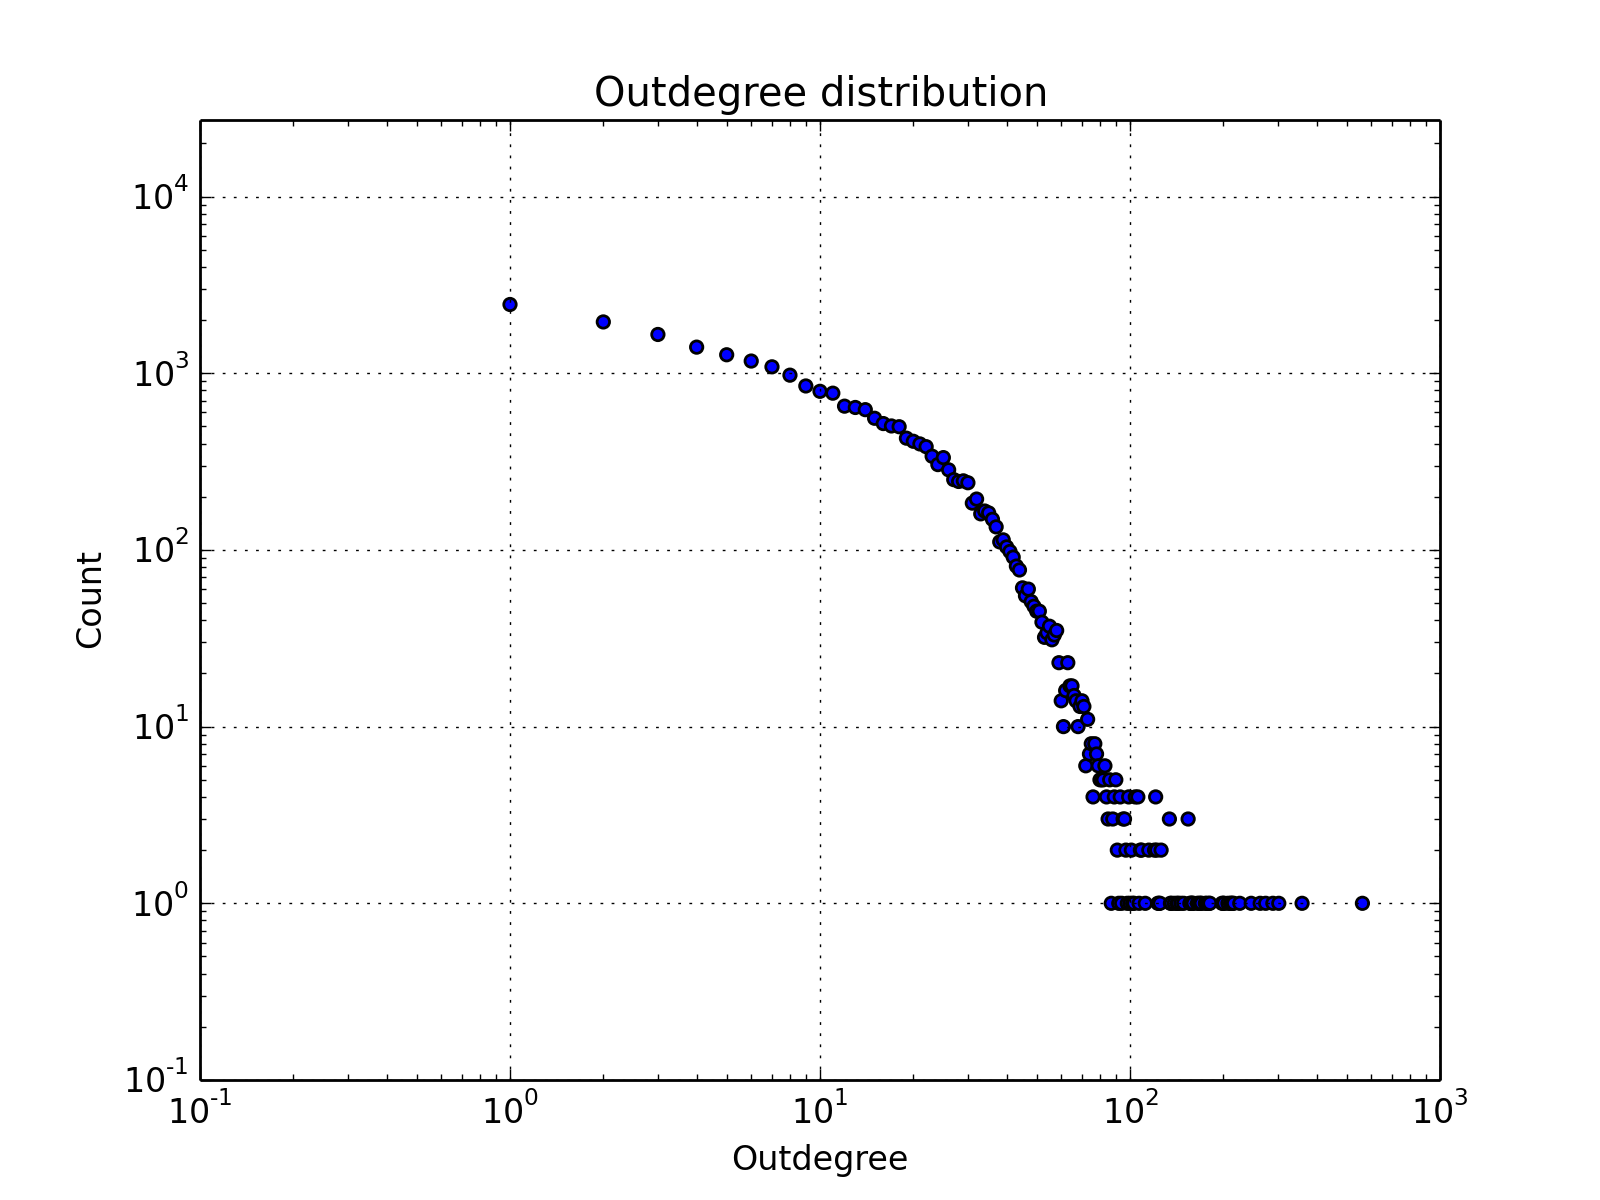
\includegraphics[width=0.35\textwidth]{FIG/OutdegreeDistoutput_cit-HepTh.png} \\
     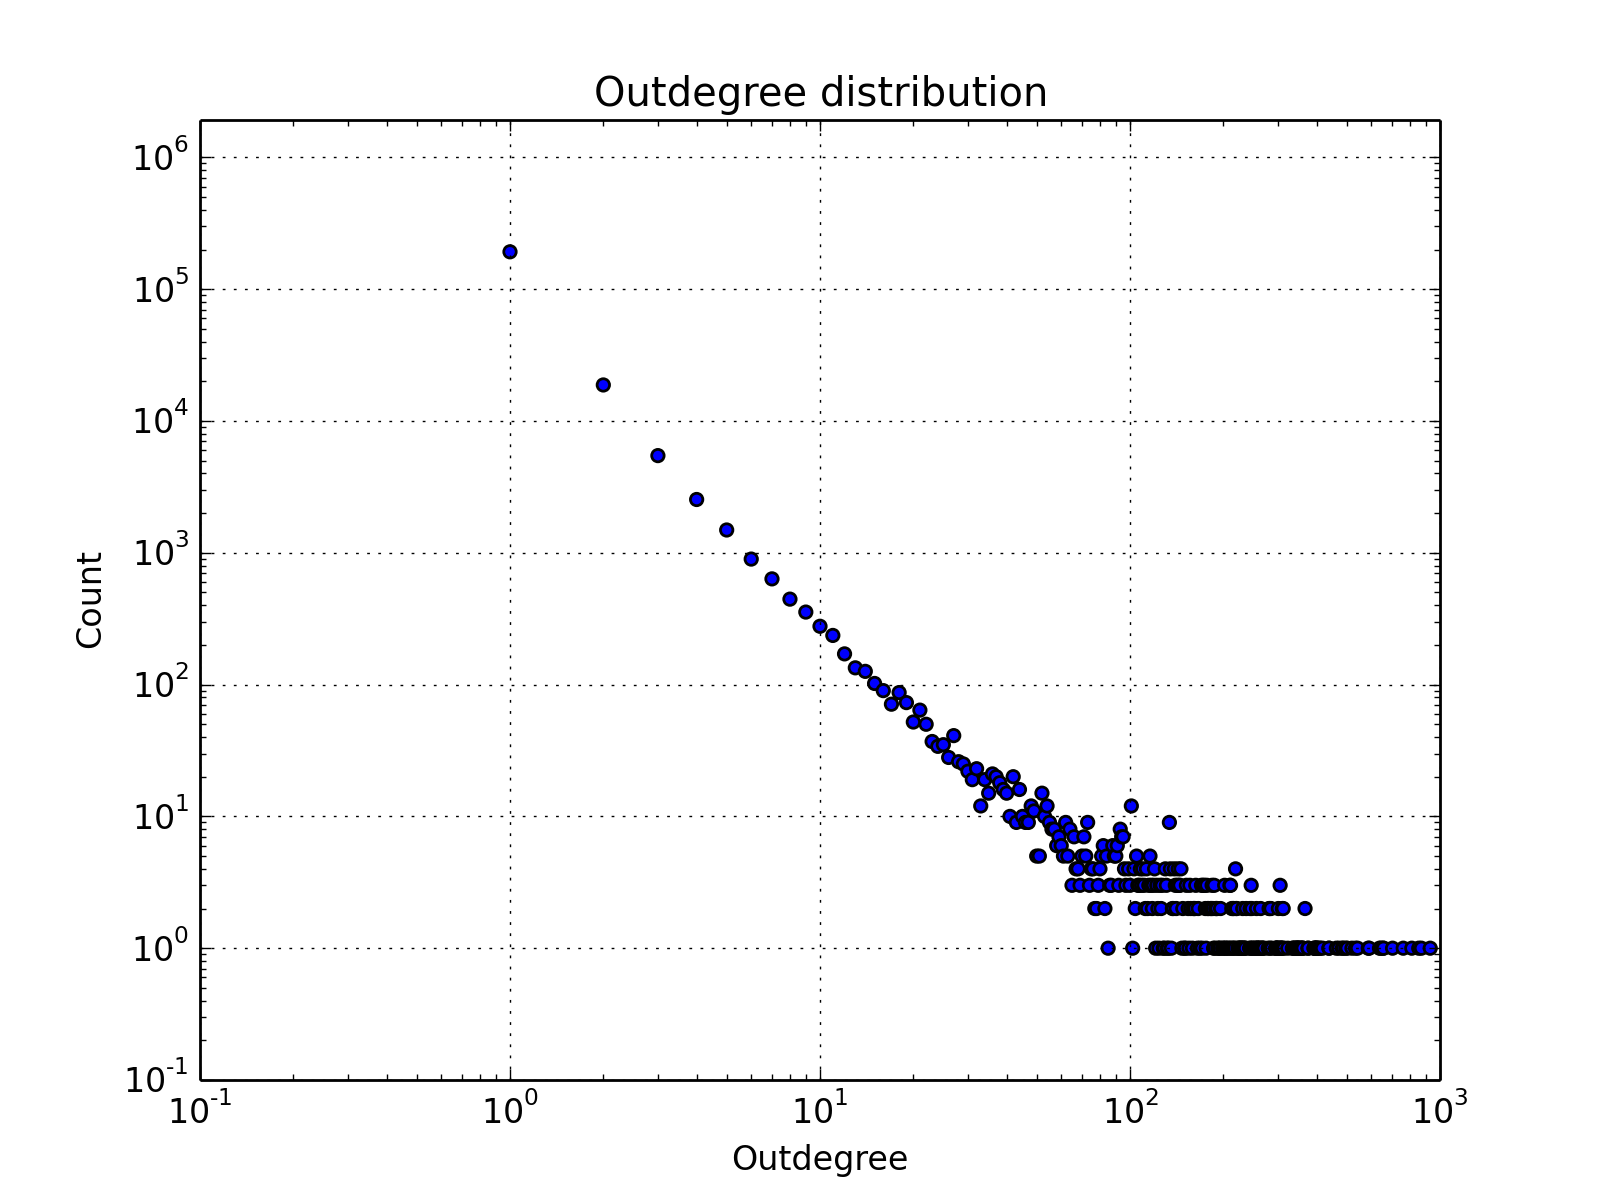
\includegraphics[width=0.35\textwidth]{FIG/OutdegreeDistoutput_email-EuAll.png} 
     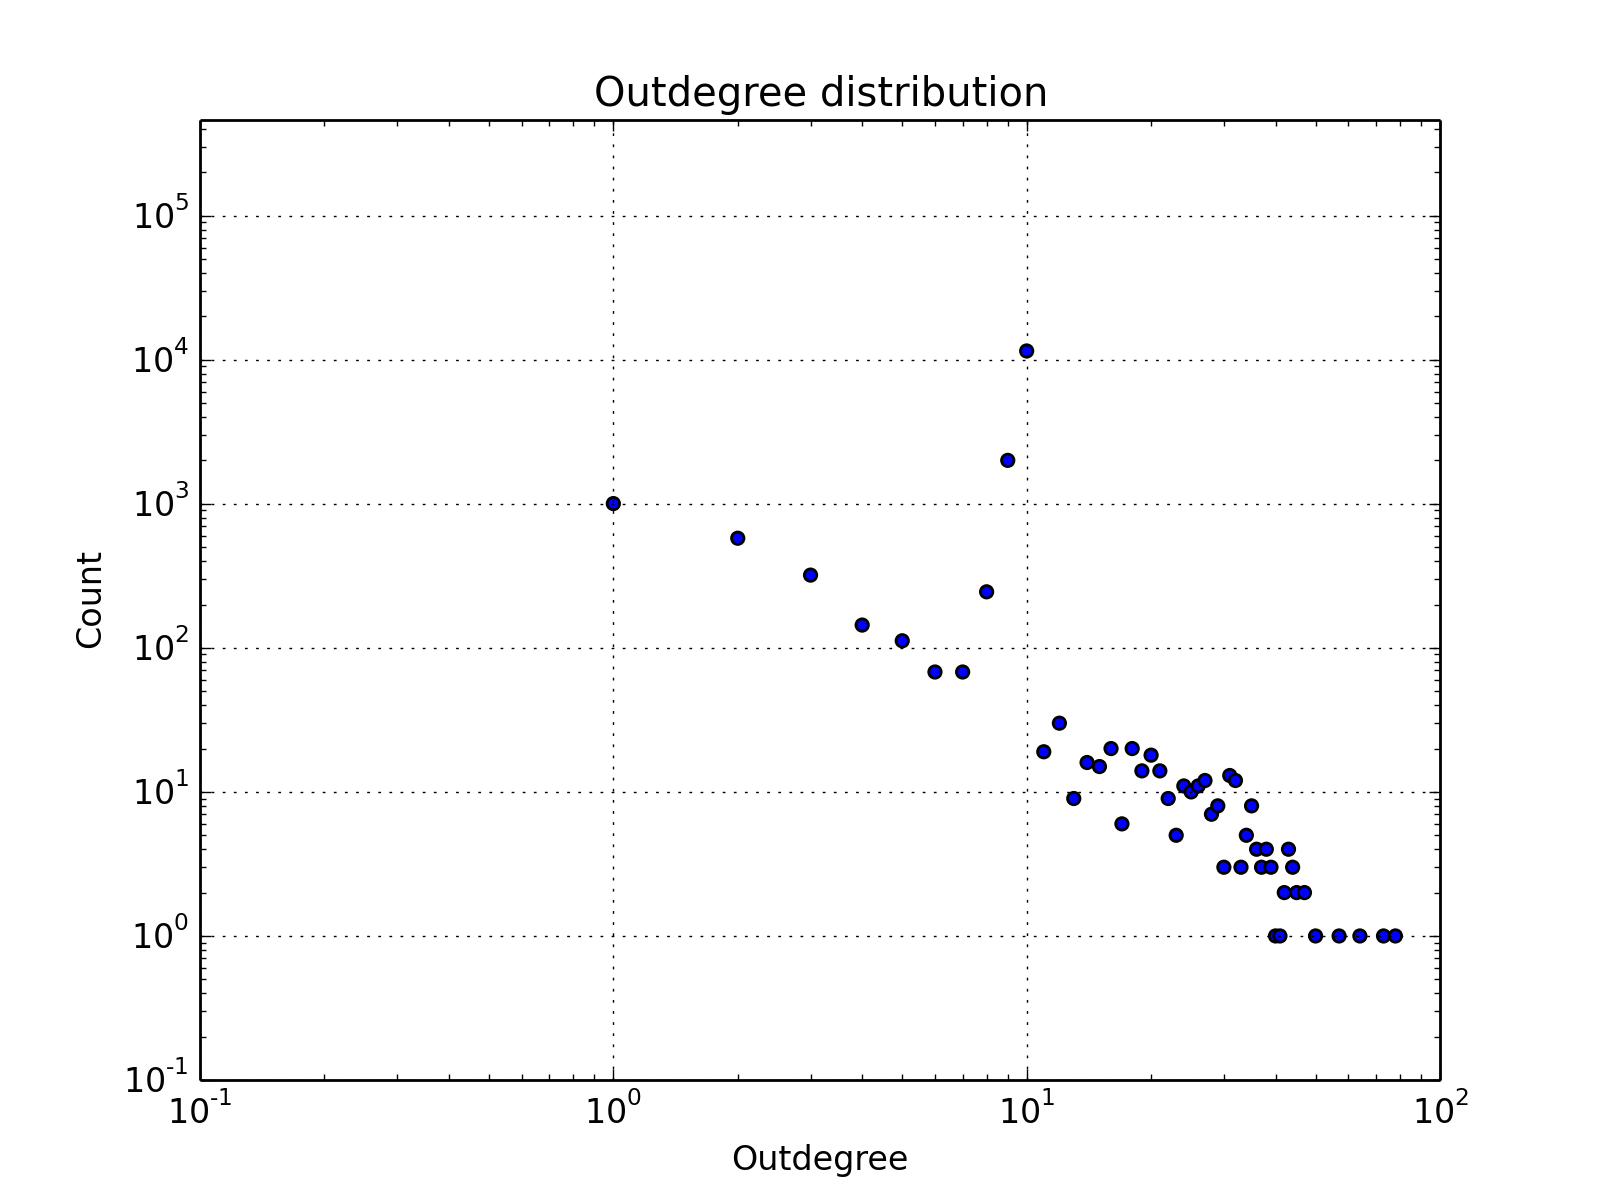
\includegraphics[width=0.35\textwidth]{FIG/OutdegreeDistoutput_p2p-Gnutella31.png} 
     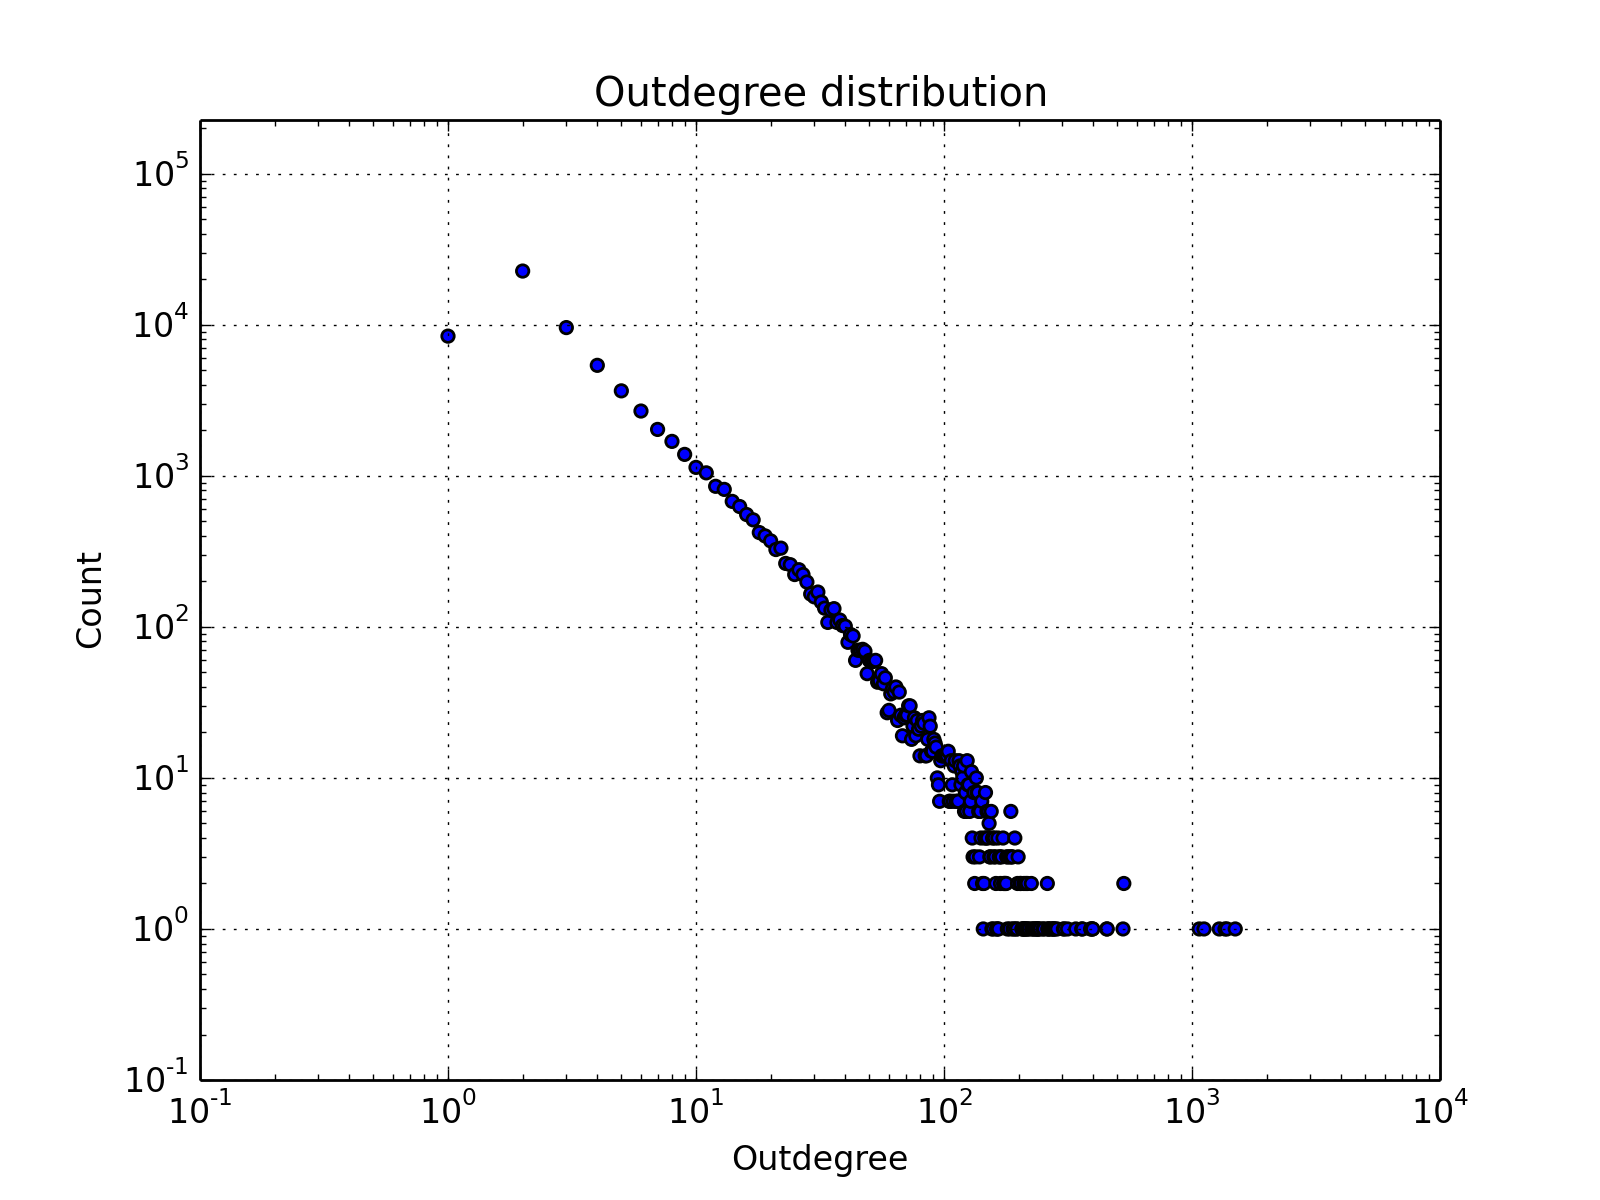
\includegraphics[width=0.35\textwidth]{FIG/OutdegreeDistoutput_soc-Slashdot0811-75000.png} 
\end{tabular}
\caption{Outdegree distribution plots of 6 directed graphs}
\label{fig:results}
\end{center}
\end{figure}

\textbf{Observation:}
\par Most graphs obey the power law, most nodes have small degree, only few nodes have high degree. In log-log space as shown above, we can draw a line to fit the scatter points.

\subsection{PageRank}
We can plot Rank vs. PageRank in log space:

\begin{figure}[H]
\begin{center}
\begin{tabular}{ccc}
     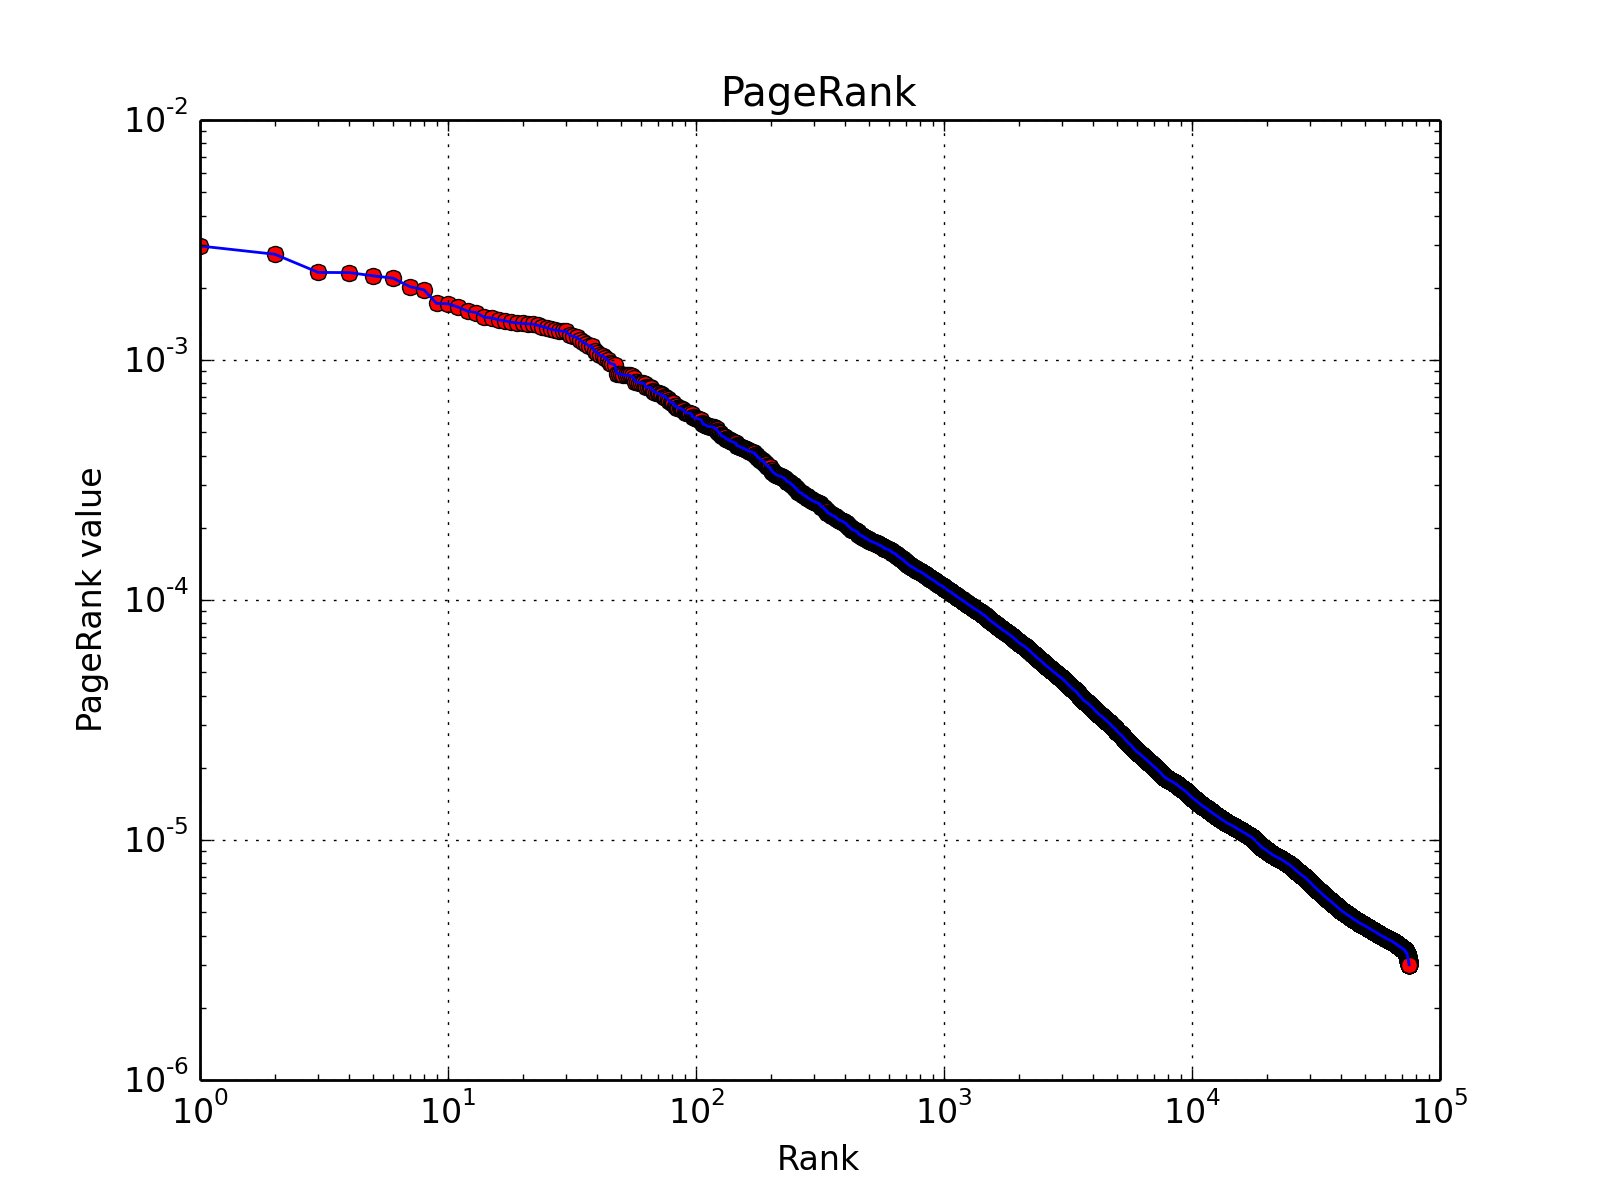
\includegraphics[width=0.35\textwidth]{FIG/pageRankoutput_as-skitter.png} 
     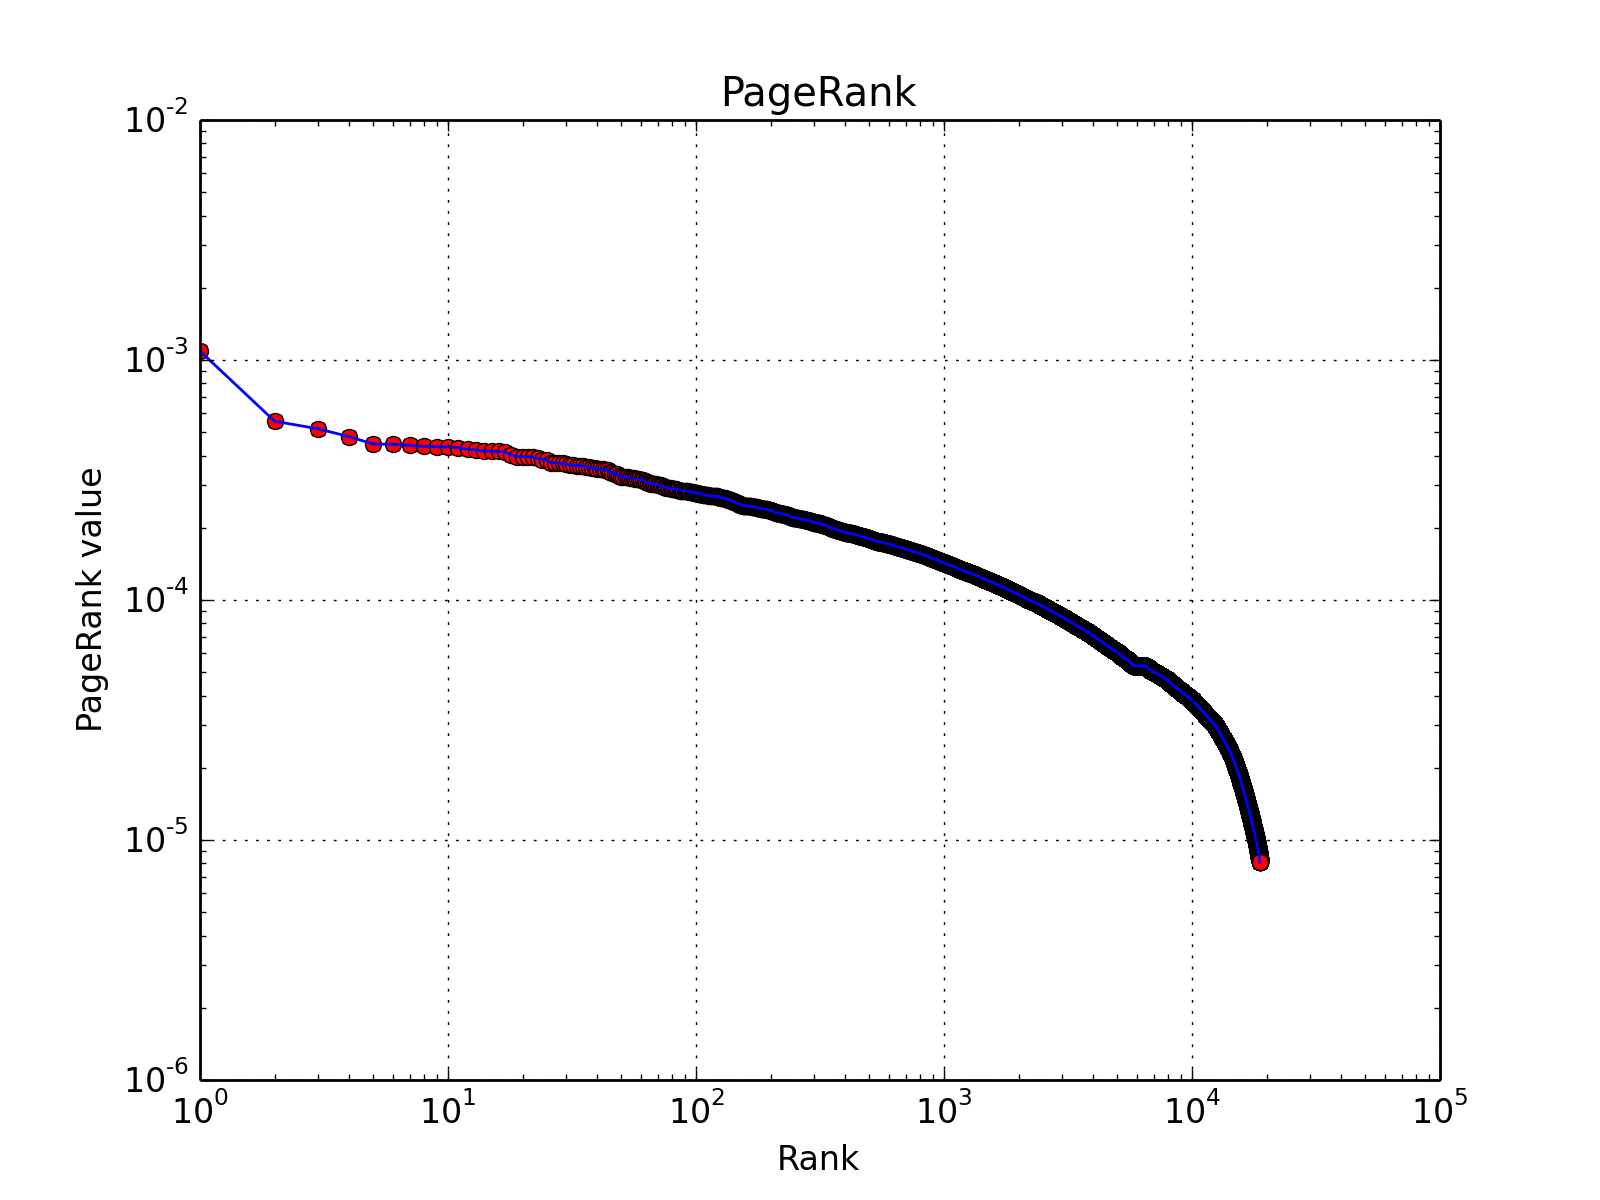
\includegraphics[width=0.35\textwidth]{FIG/pageRankoutput_ca-AstroPh.png}
     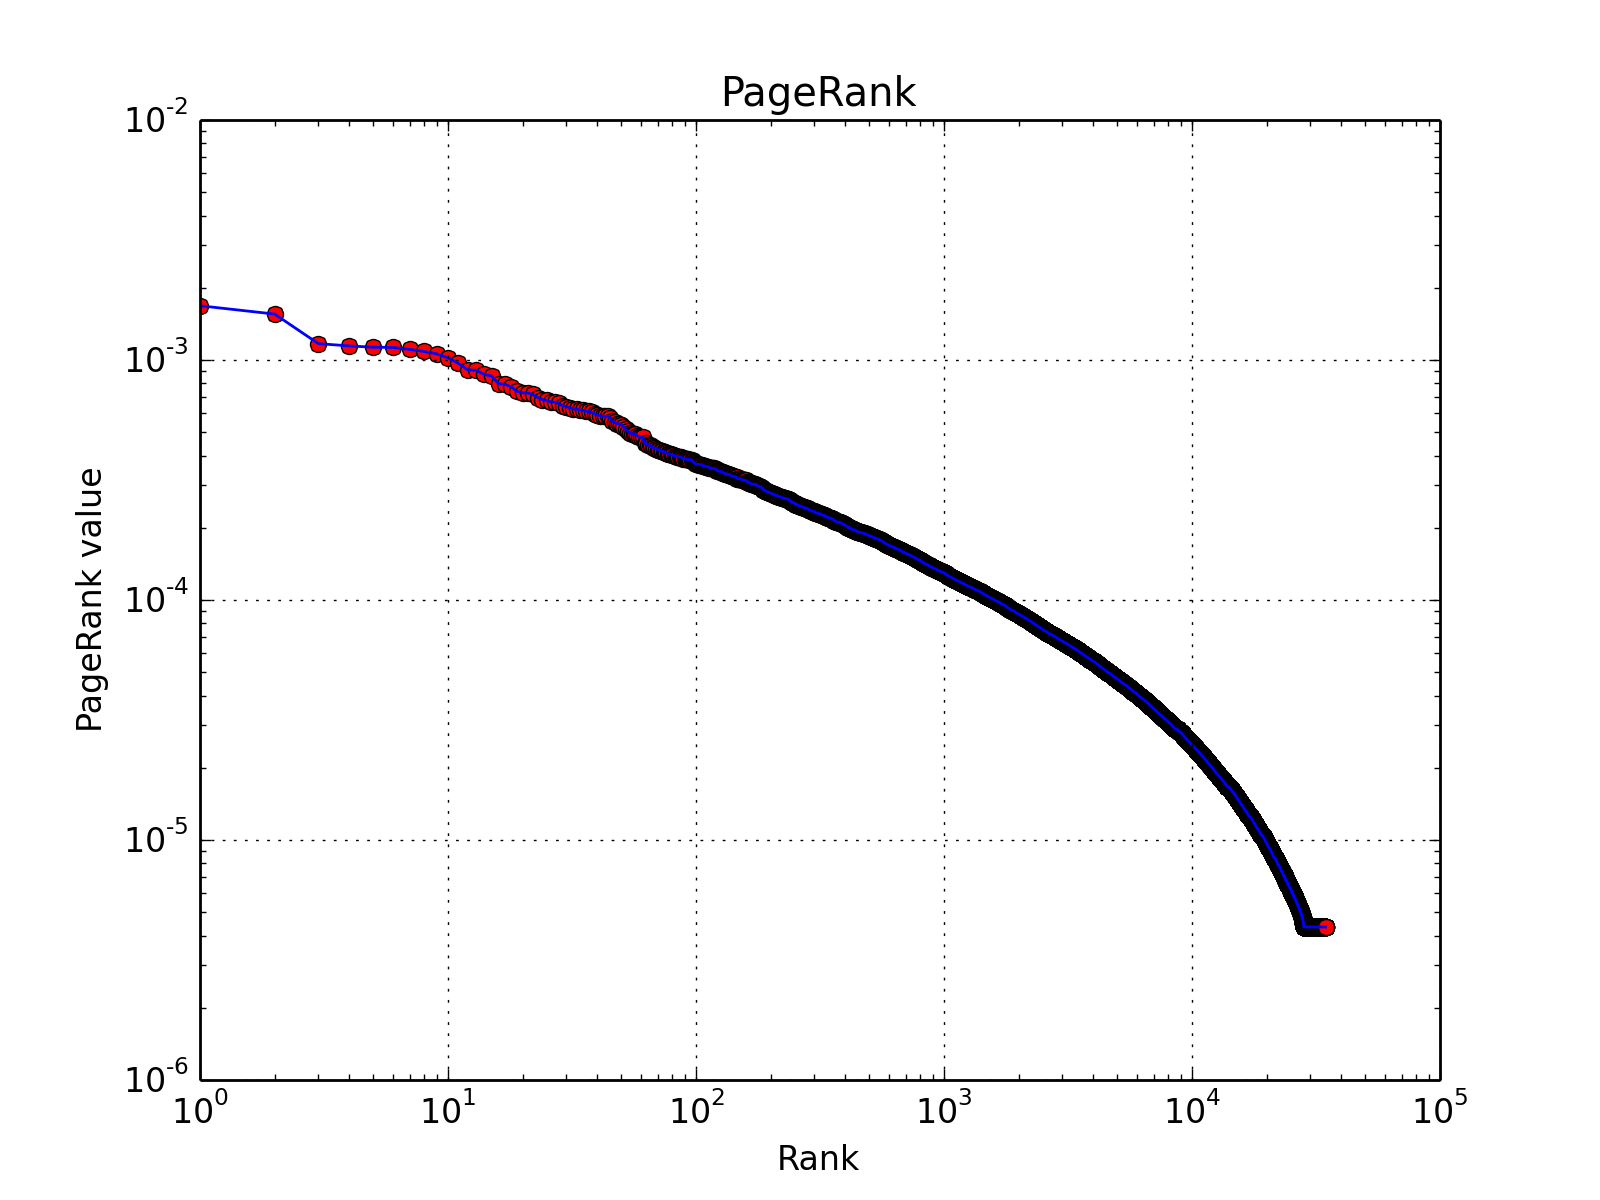
\includegraphics[width=0.35\textwidth]{FIG/pageRankoutput_cit-HepPh.png} \\
     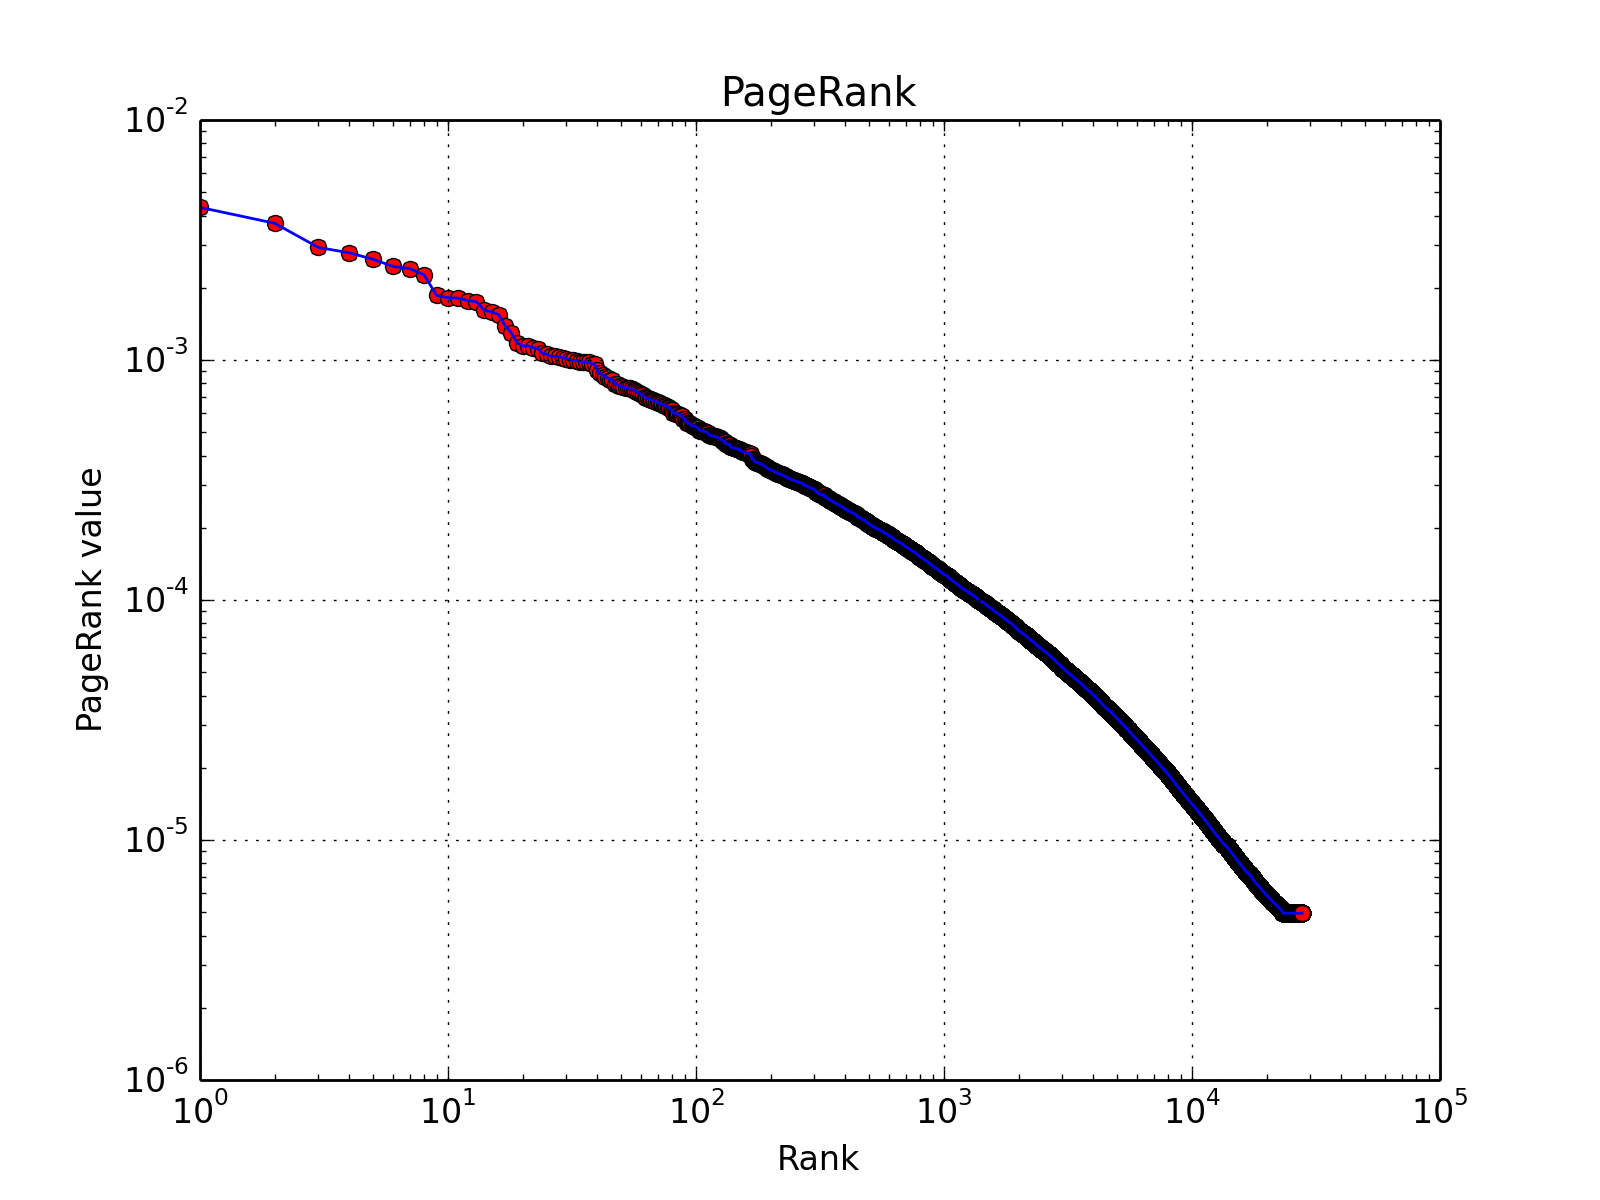
\includegraphics[width=0.35\textwidth]{FIG/pageRankoutput_cit-HepTh.png} 
     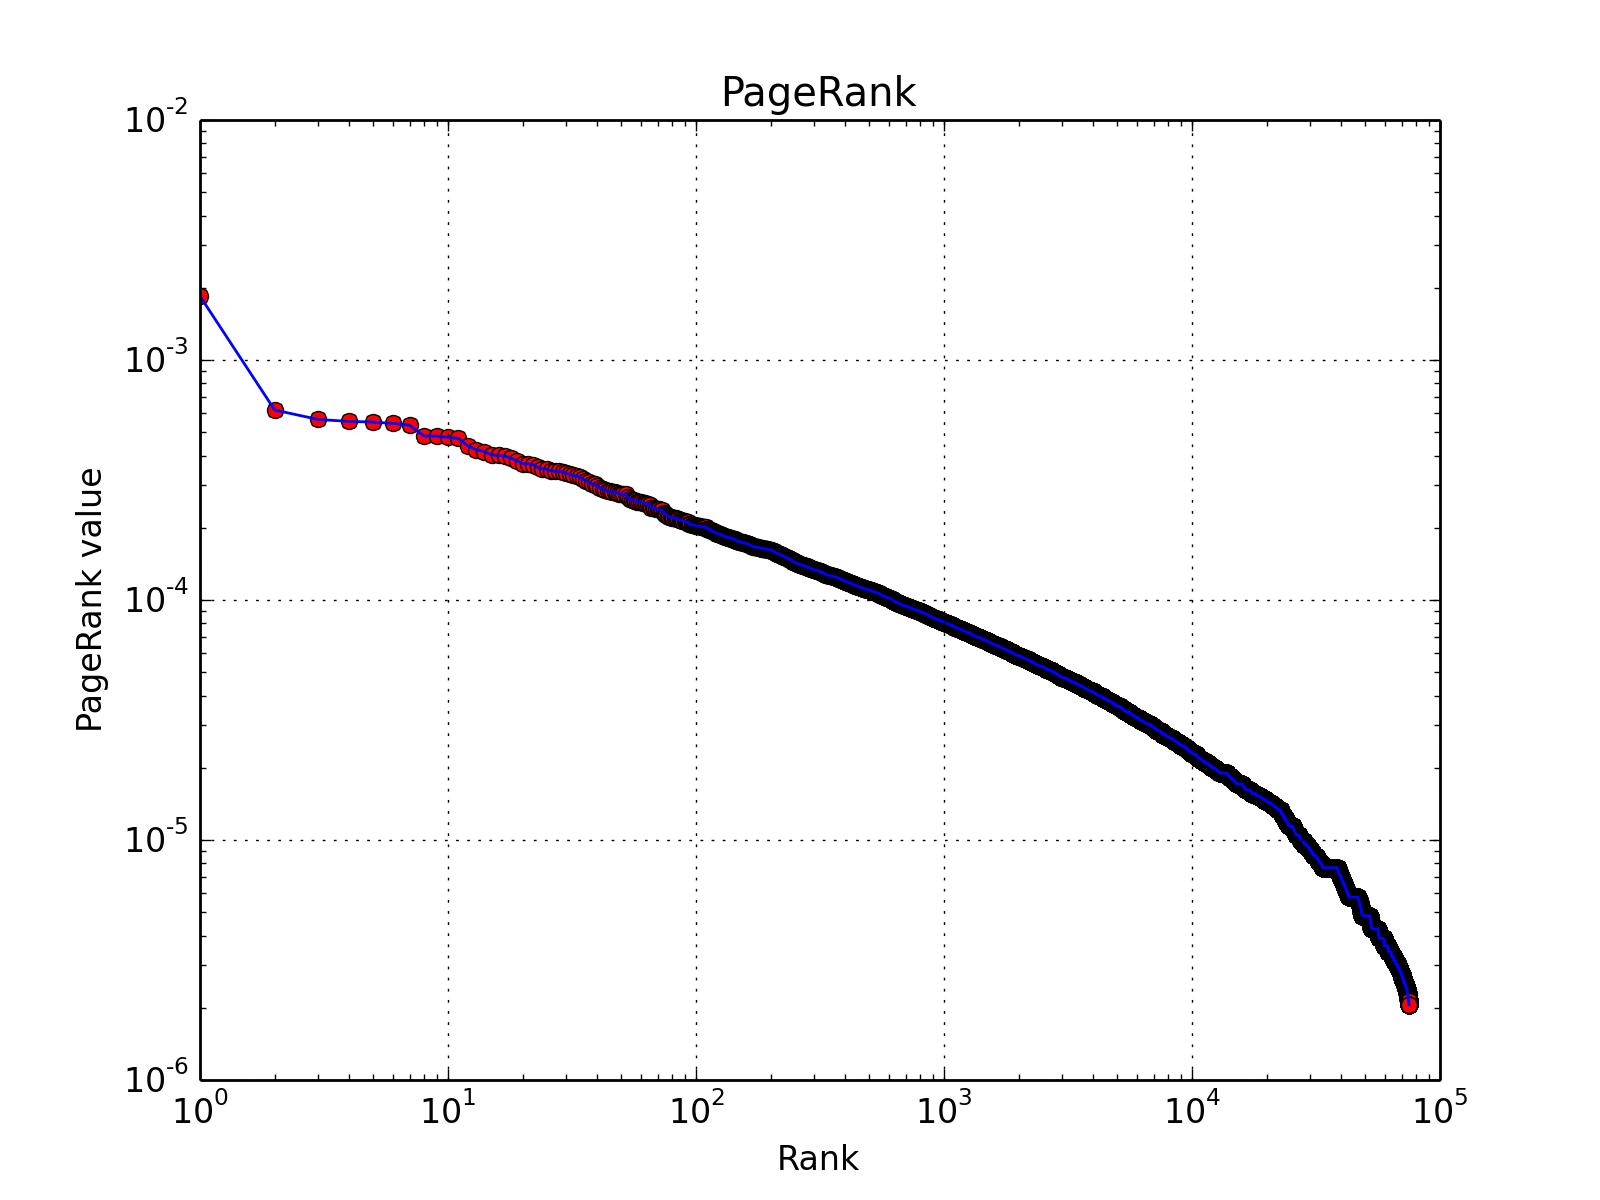
\includegraphics[width=0.35\textwidth]{FIG/pageRankoutput_com-amazon.png} 
     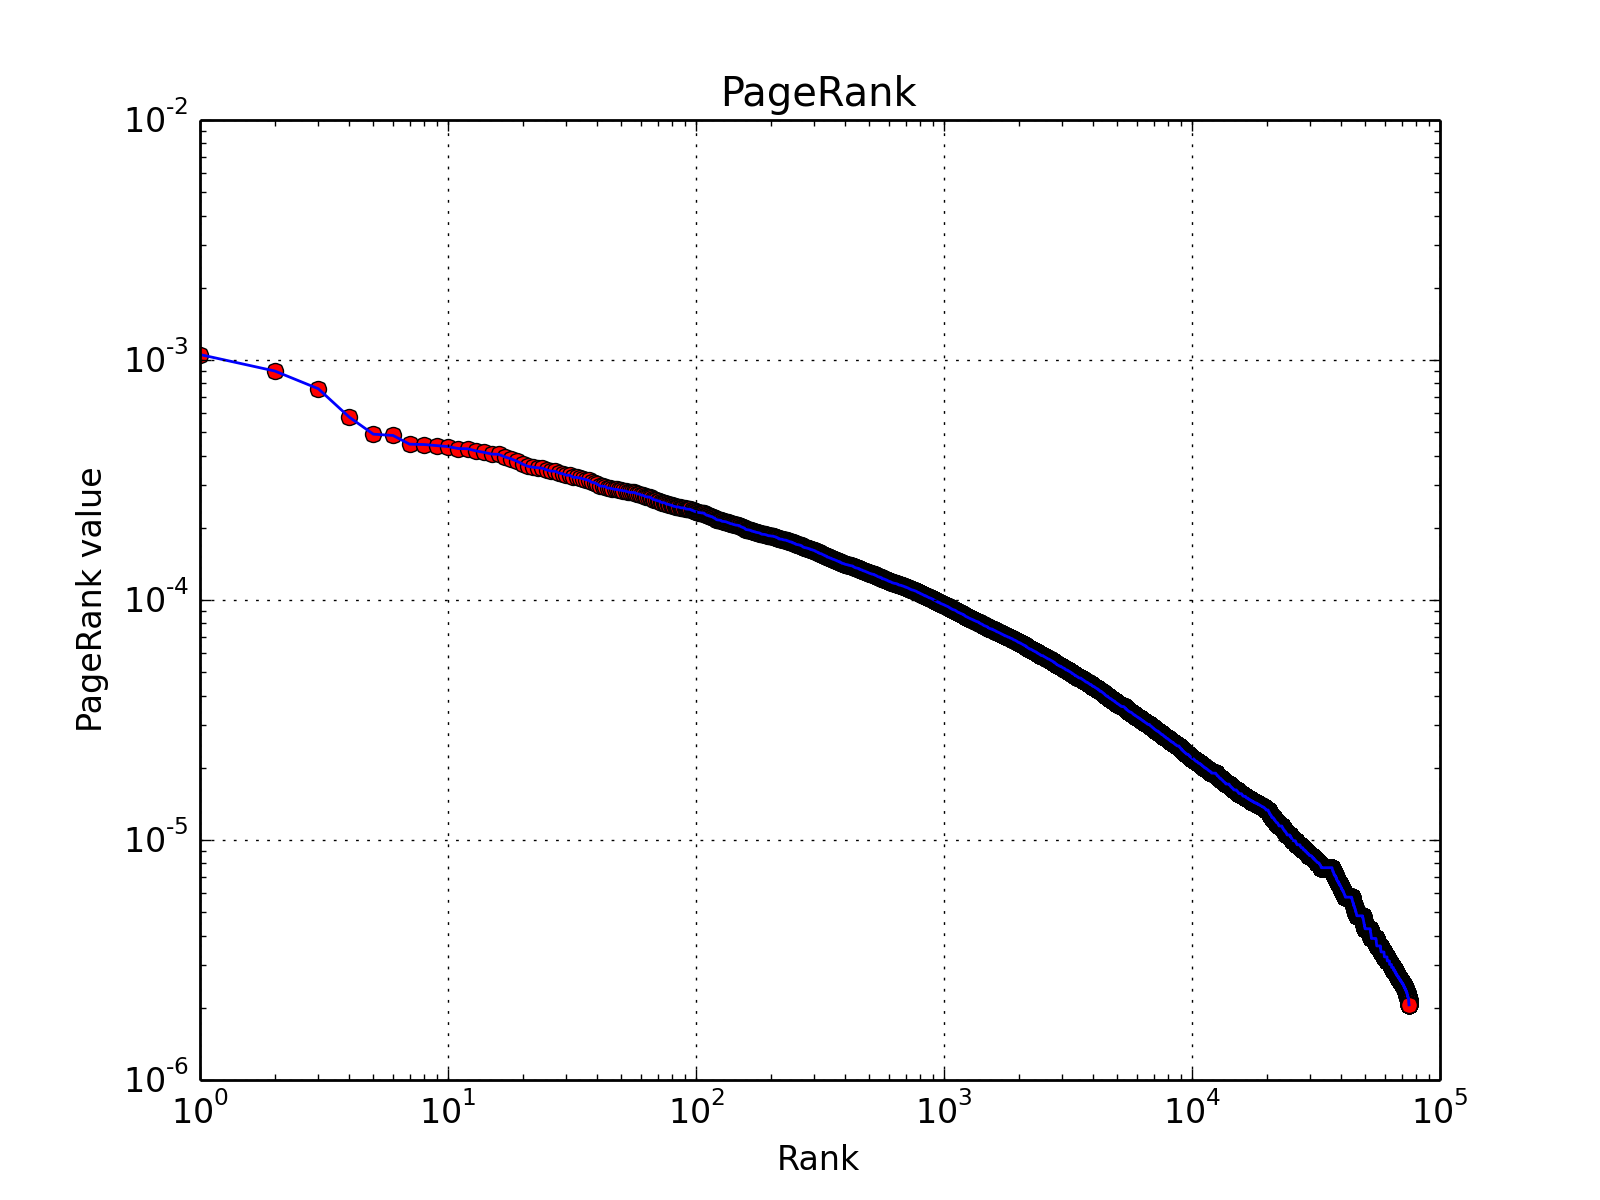
\includegraphics[width=0.35\textwidth]{FIG/pageRankoutput_com-dblp.png} \\
     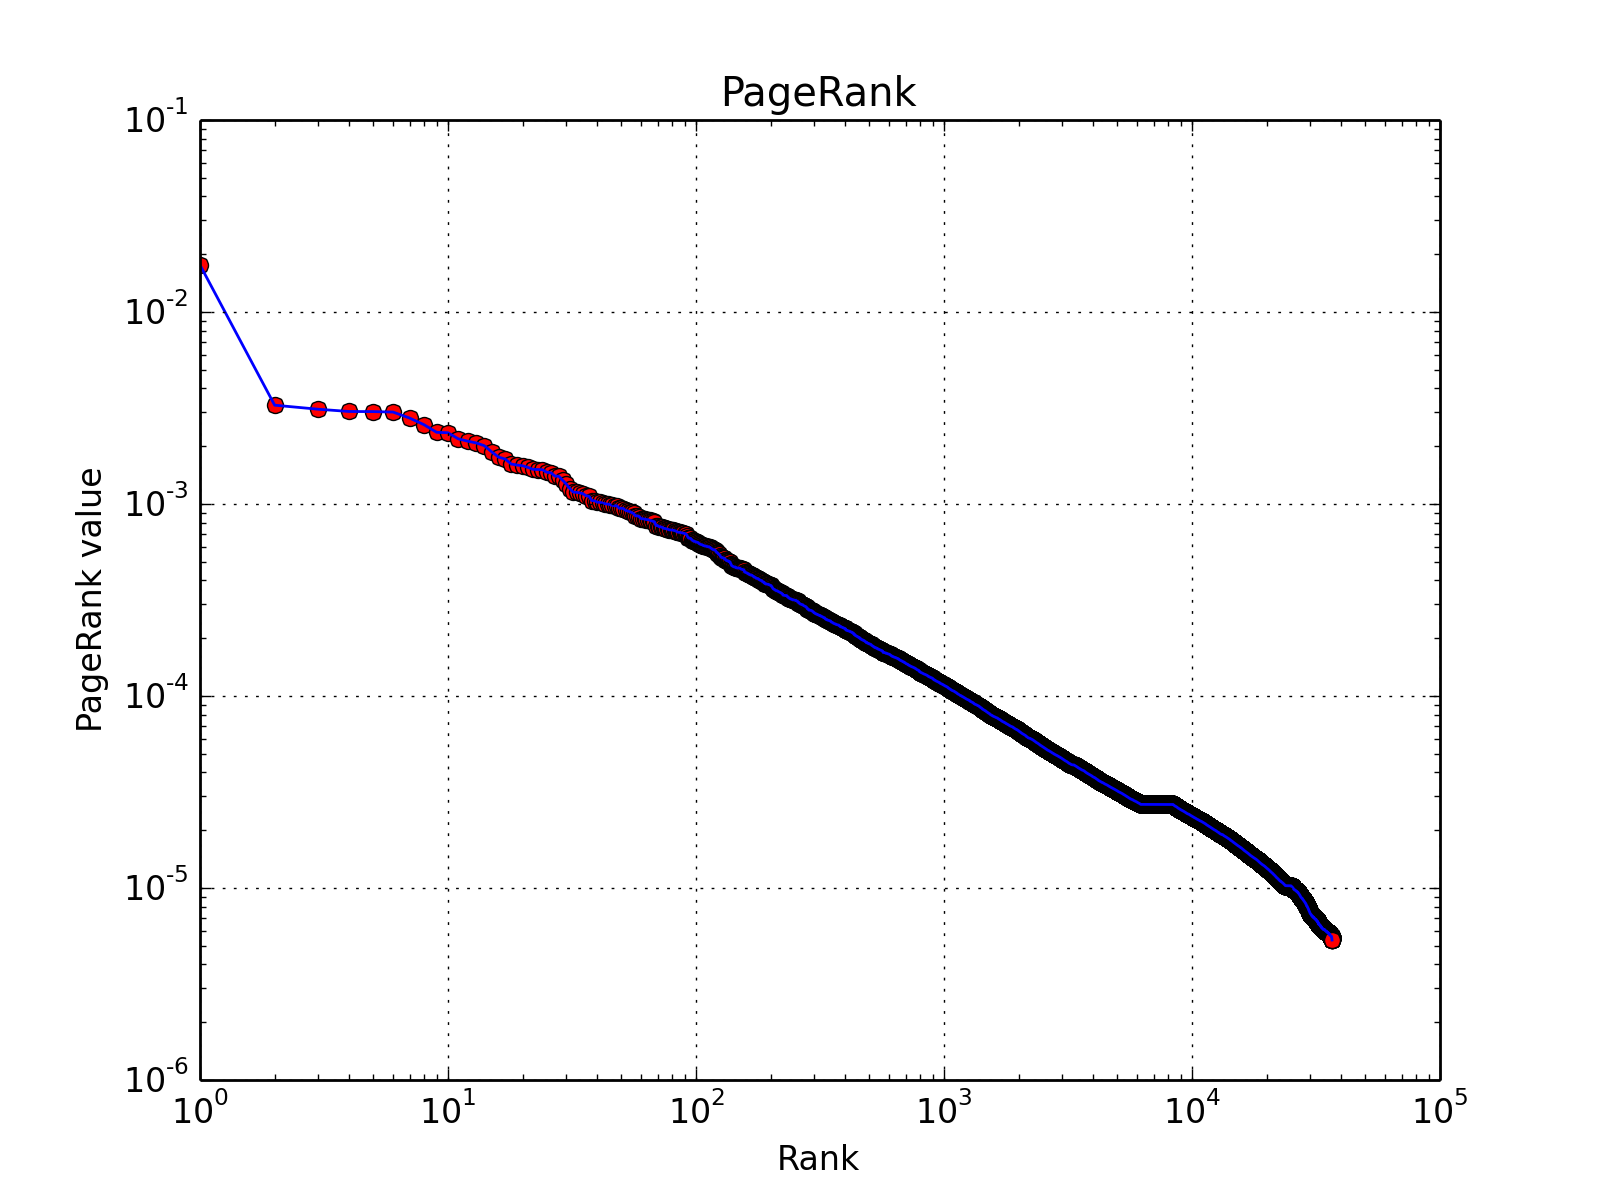
\includegraphics[width=0.35\textwidth]{FIG/pageRankoutput_email-Enron.png} 
     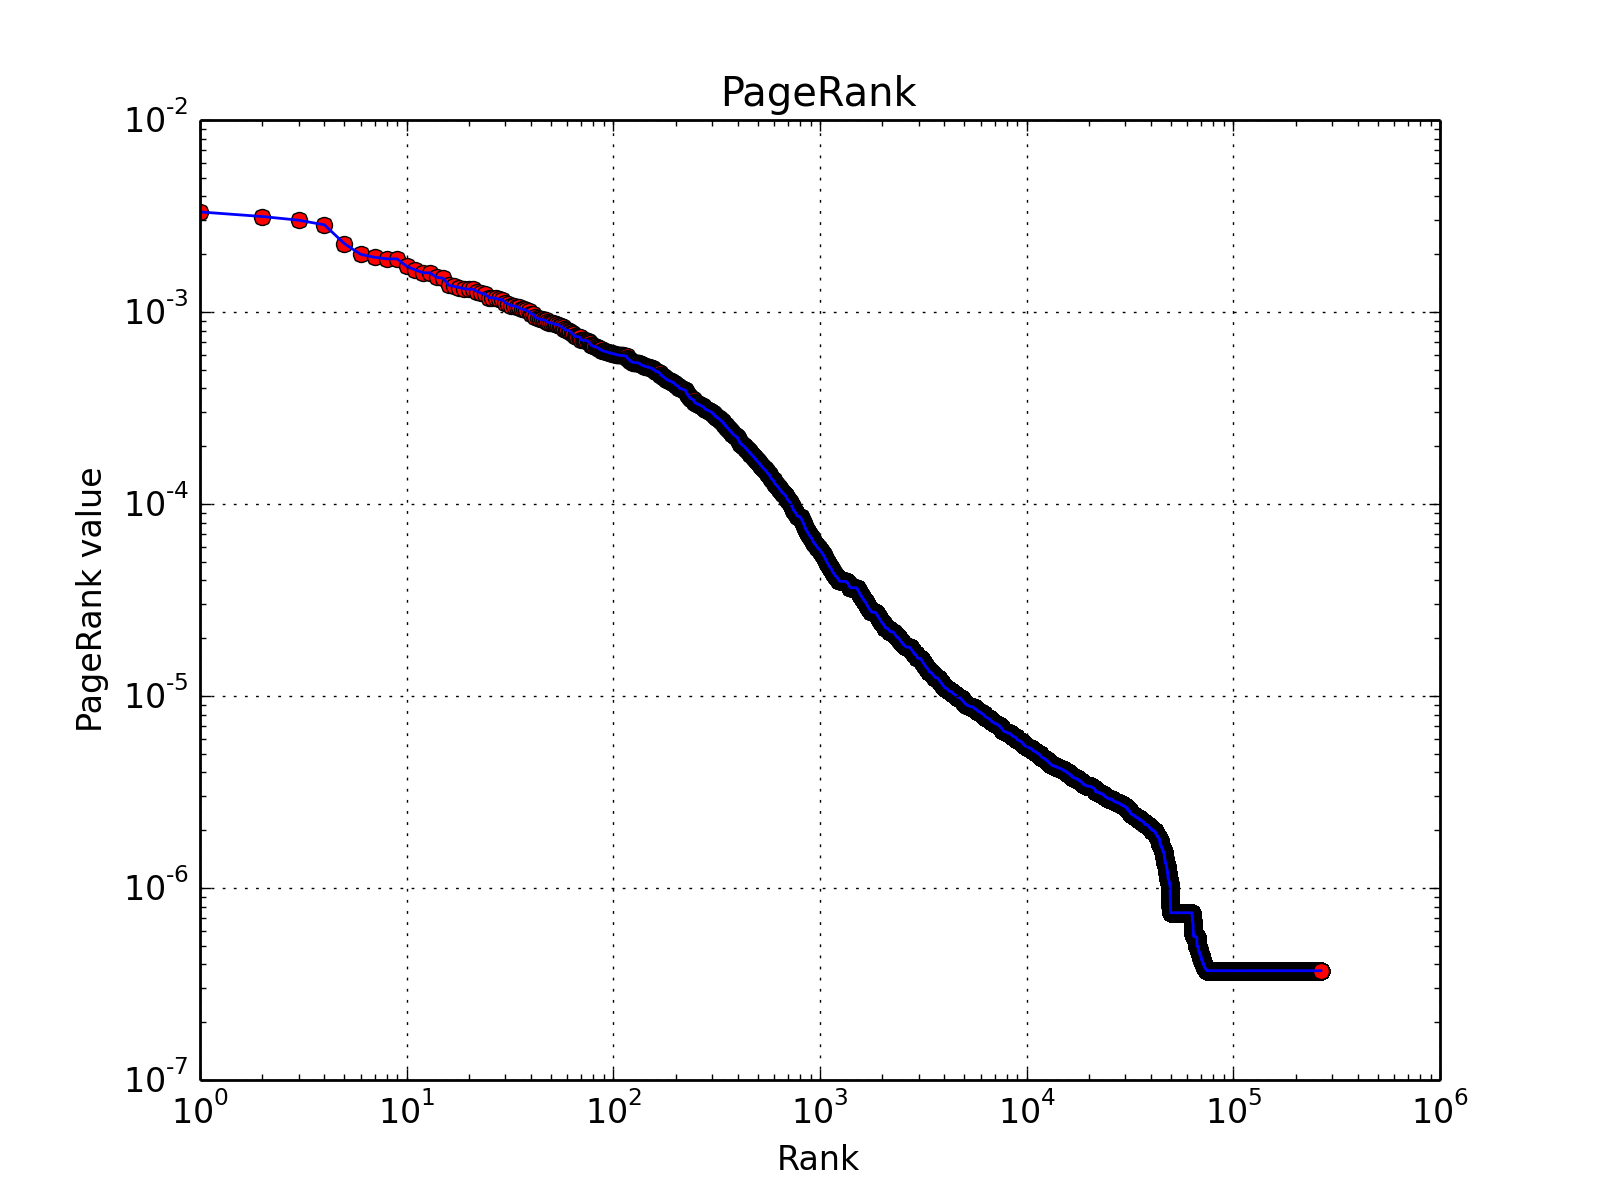
\includegraphics[width=0.35\textwidth]{FIG/pageRankoutput_email-EuAll.png} 
     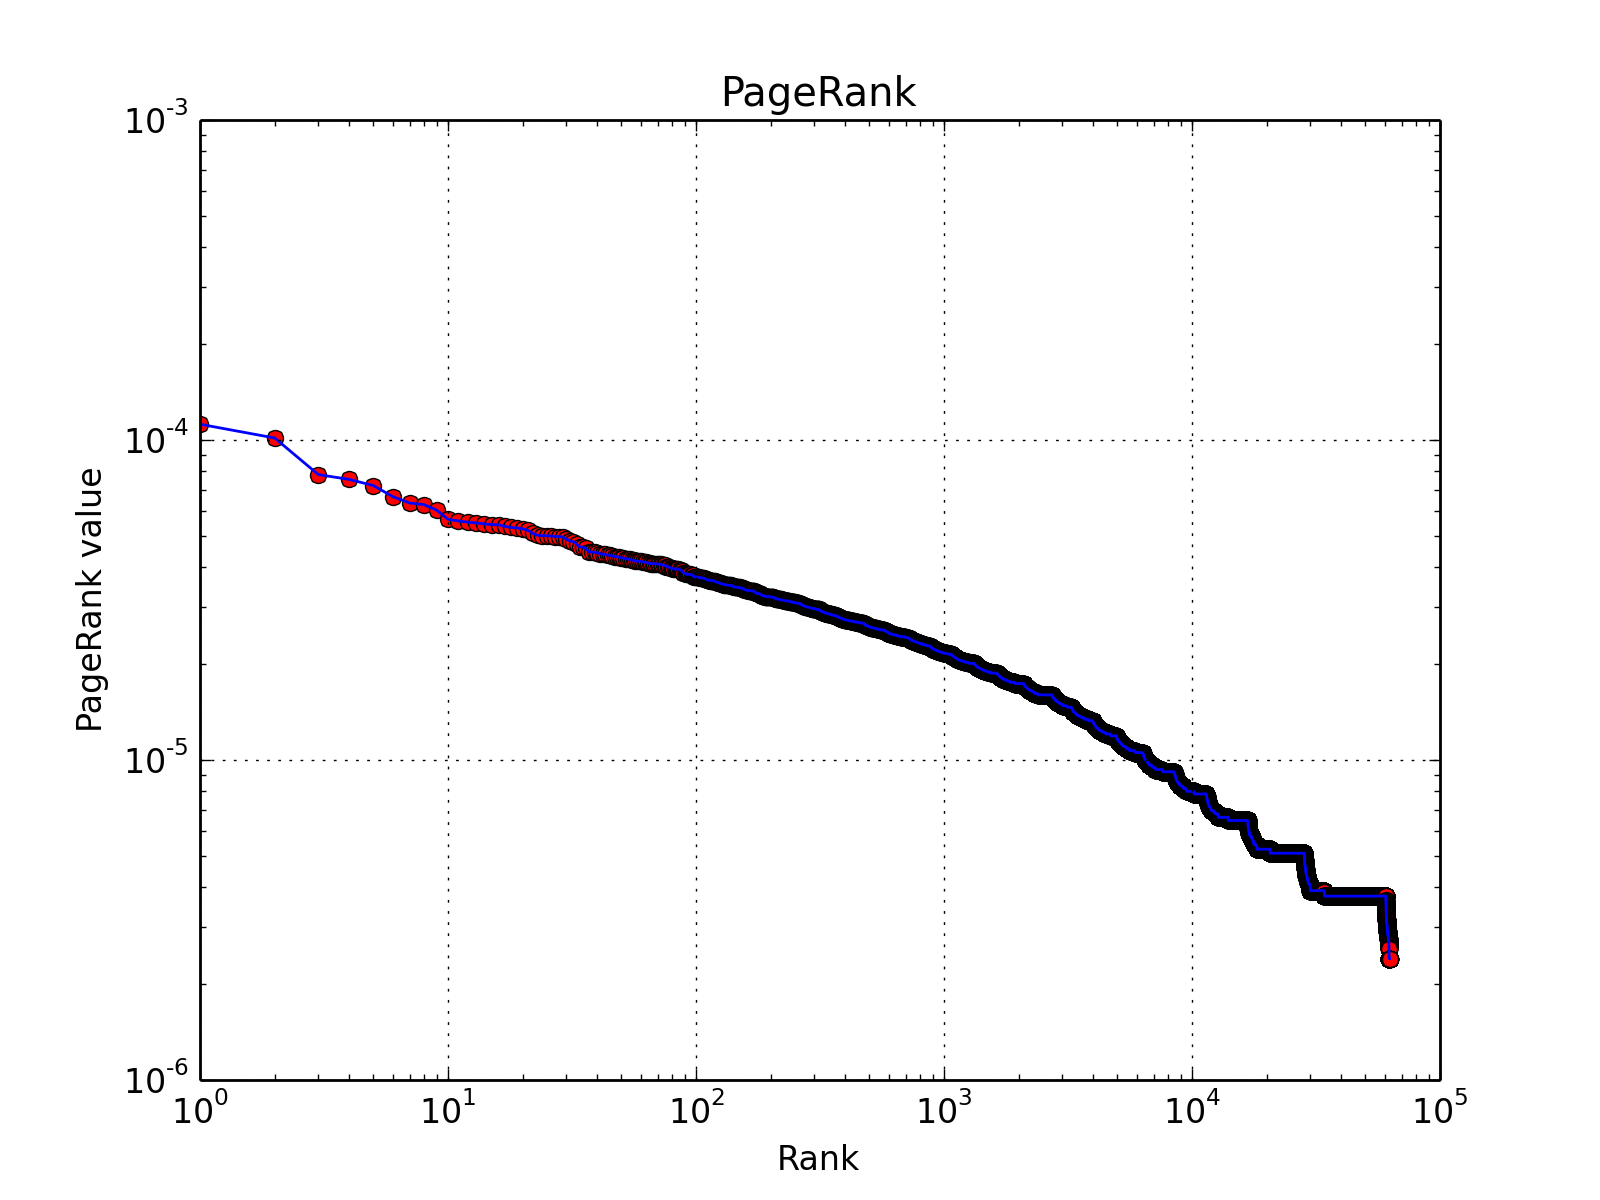
\includegraphics[width=0.35\textwidth]{FIG/pageRankoutput_p2p-Gnutella31.png} \\
     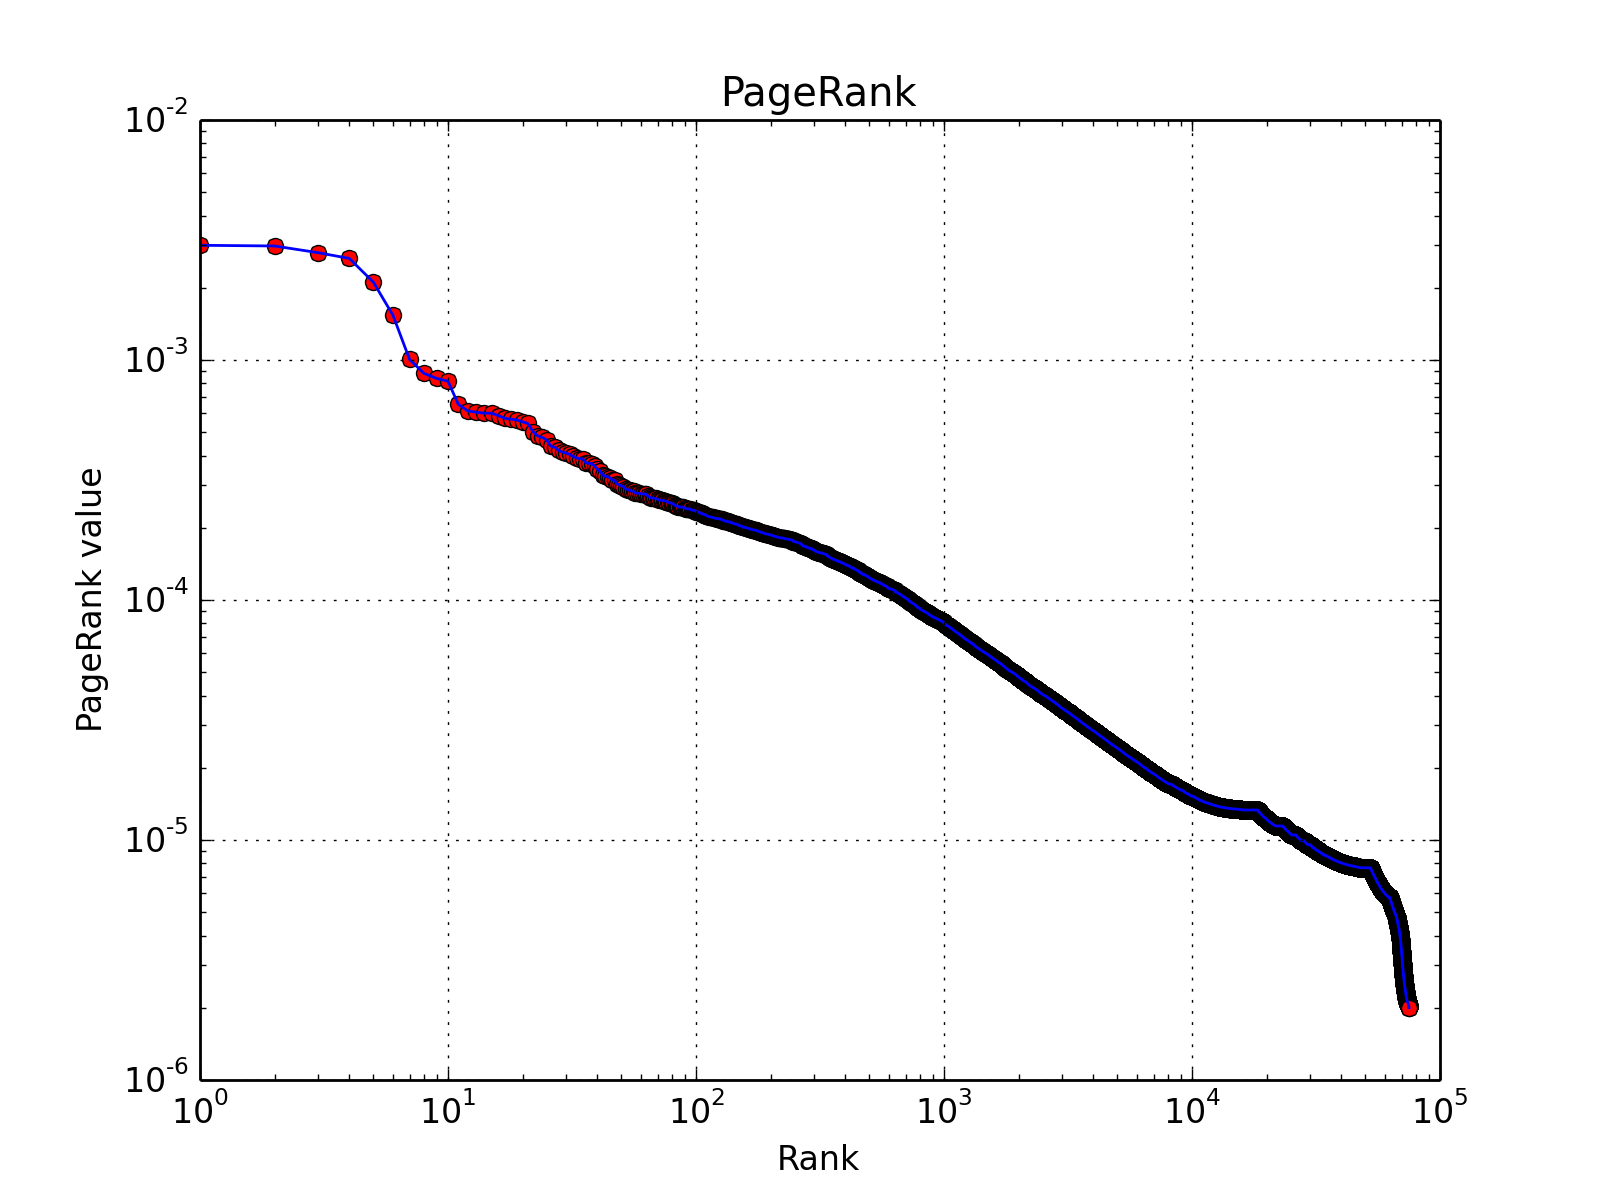
\includegraphics[width=0.35\textwidth]{FIG/pageRankoutput_soc-Slashdot0811-75000.png} 
\end{tabular}
\caption{PageRank plots of 10 graphs}
\label{fig:results}
\end{center}
\end{figure}

\textbf{Observation:}
\par Rank and PageRank of most graphs obey the power law. In log-log space as shown above, we can draw a line to fit the scatter points.

\subsection{Weakly connected components}

\begin{figure}[H]
\begin{center}
\begin{tabular}{ccc}
     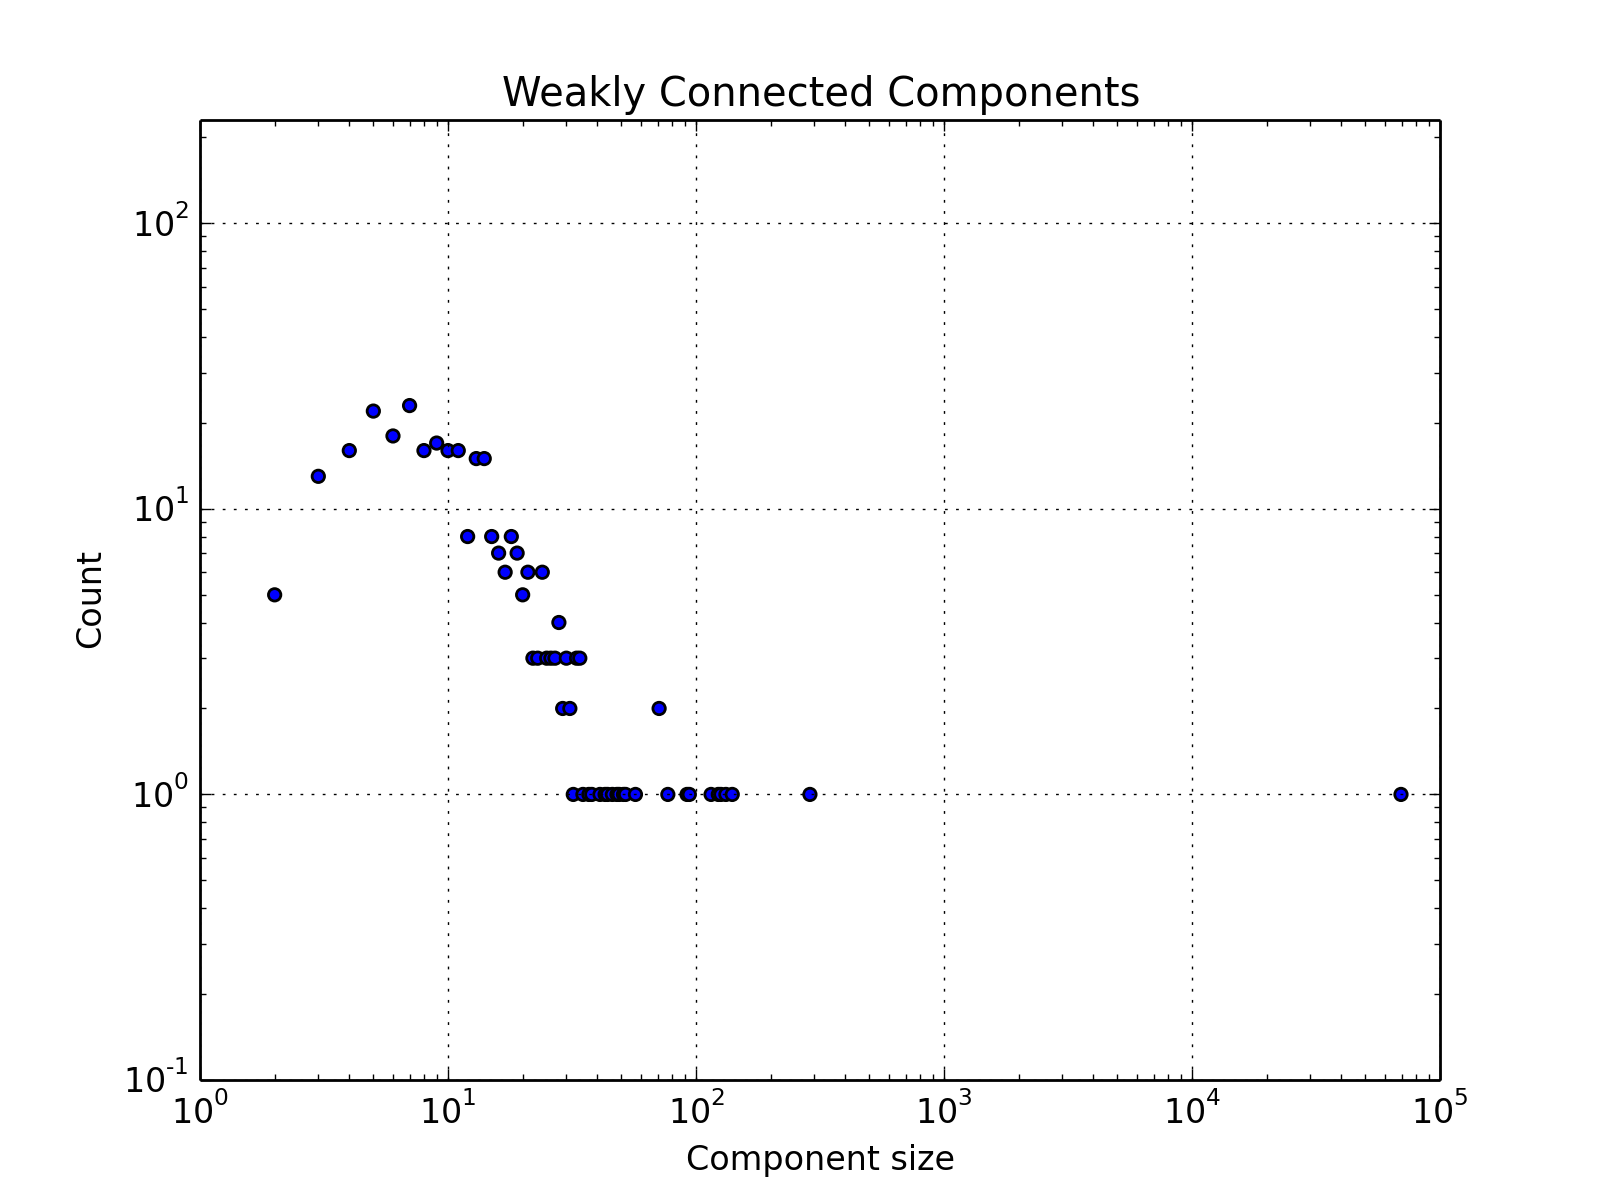
\includegraphics[width=0.35\textwidth]{FIG/plotConncompoutput_as-skitter.png} 
     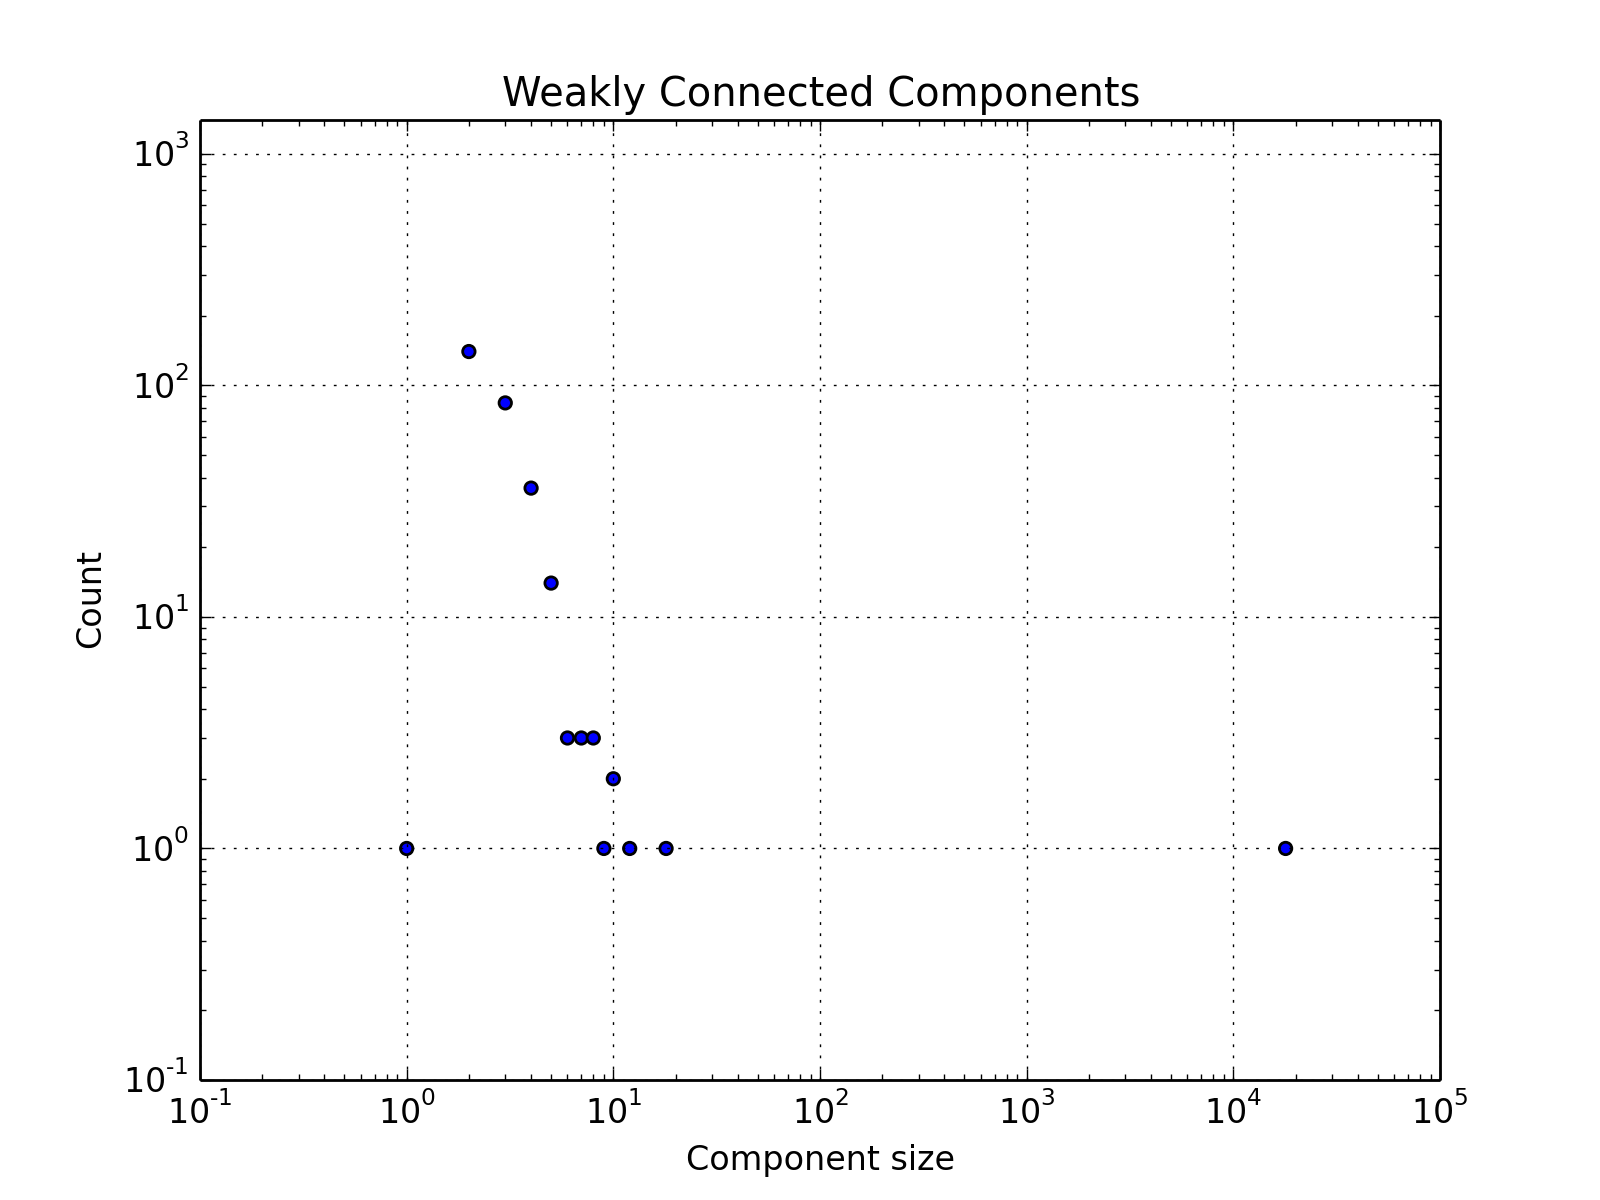
\includegraphics[width=0.35\textwidth]{FIG/plotConncompoutput_ca-AstroPh.png}
     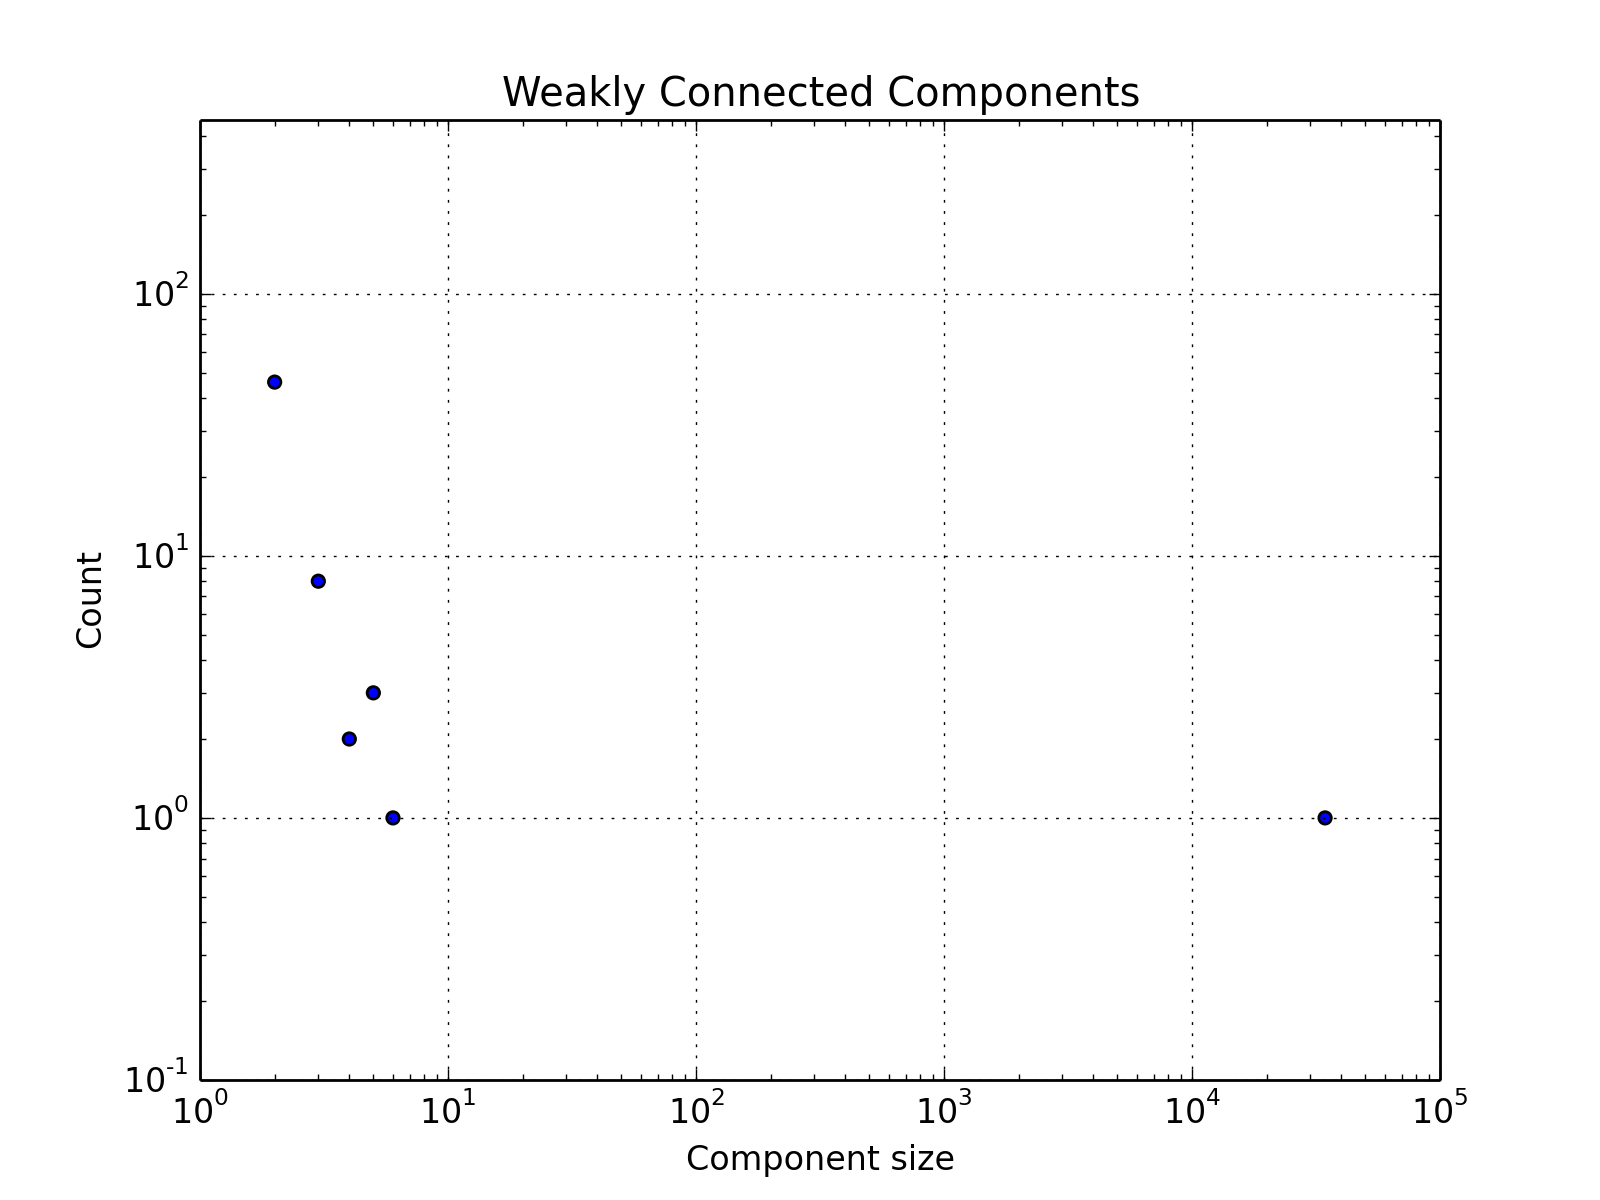
\includegraphics[width=0.35\textwidth]{FIG/plotConncompoutput_cit-HepPh.png} \\
     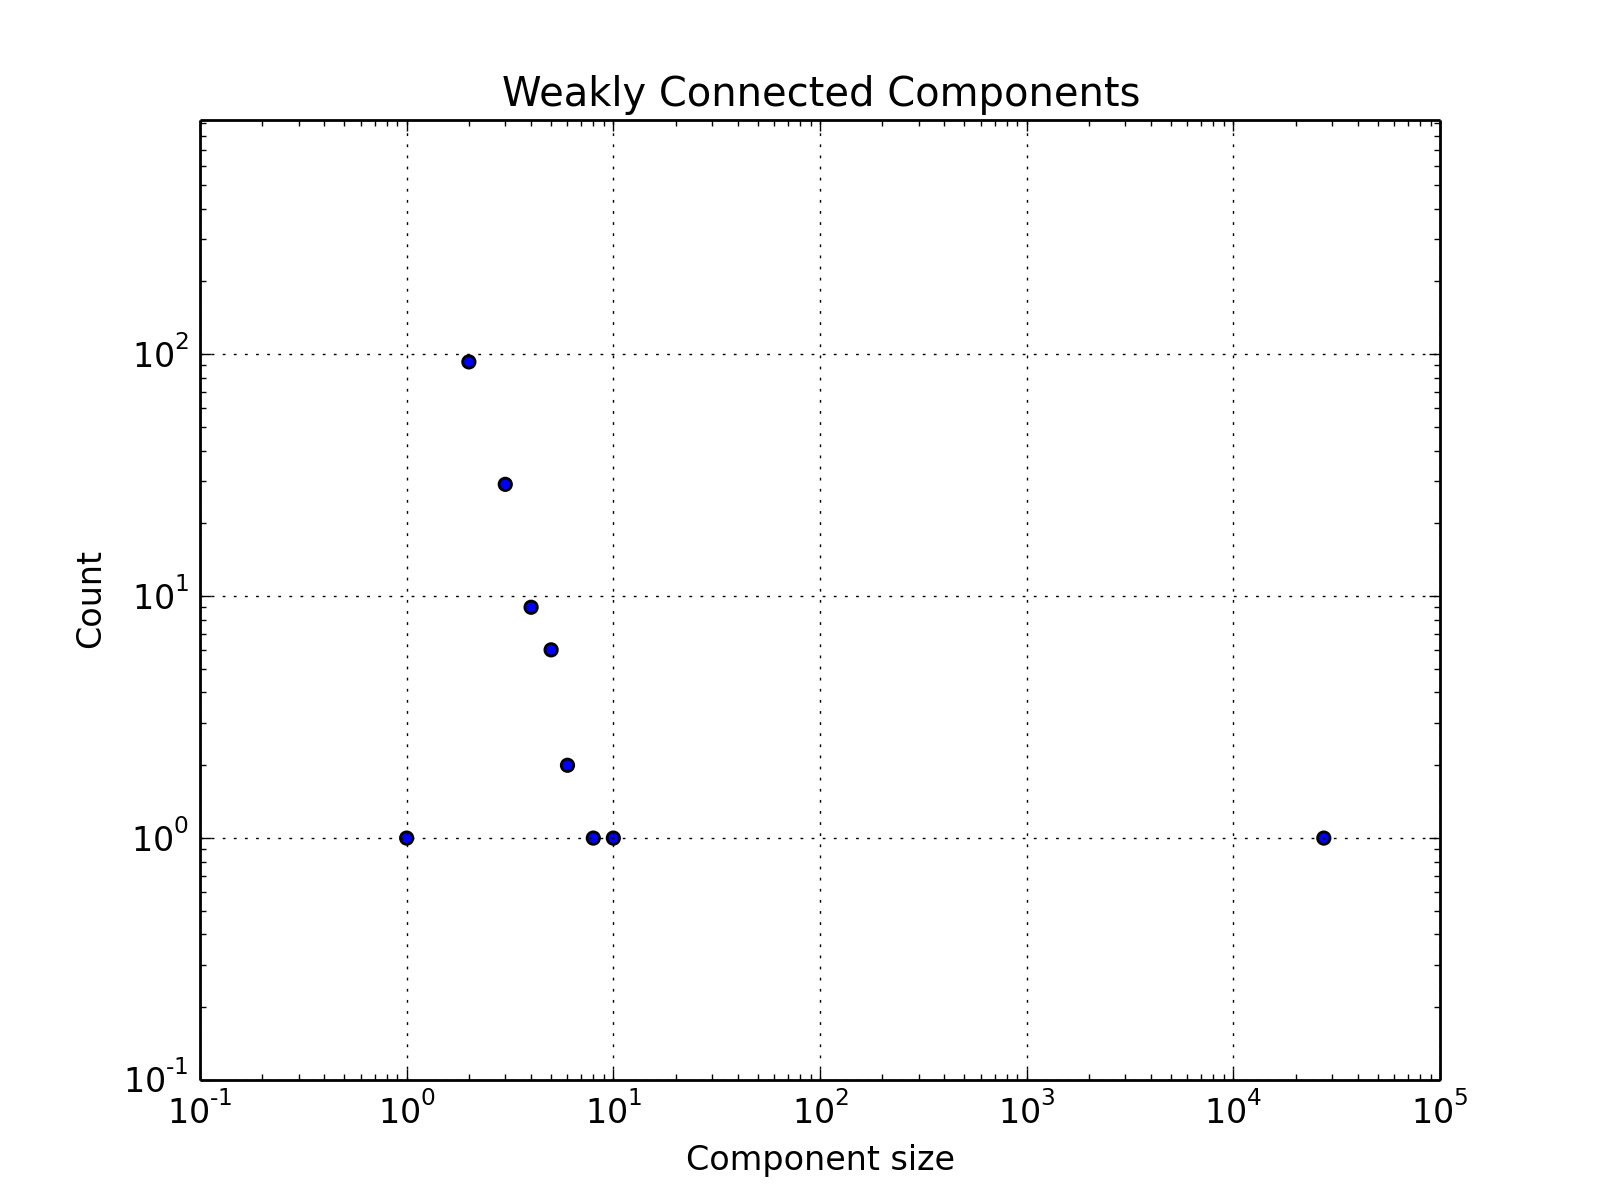
\includegraphics[width=0.35\textwidth]{FIG/plotConncompoutput_cit-HepTh.png} 
     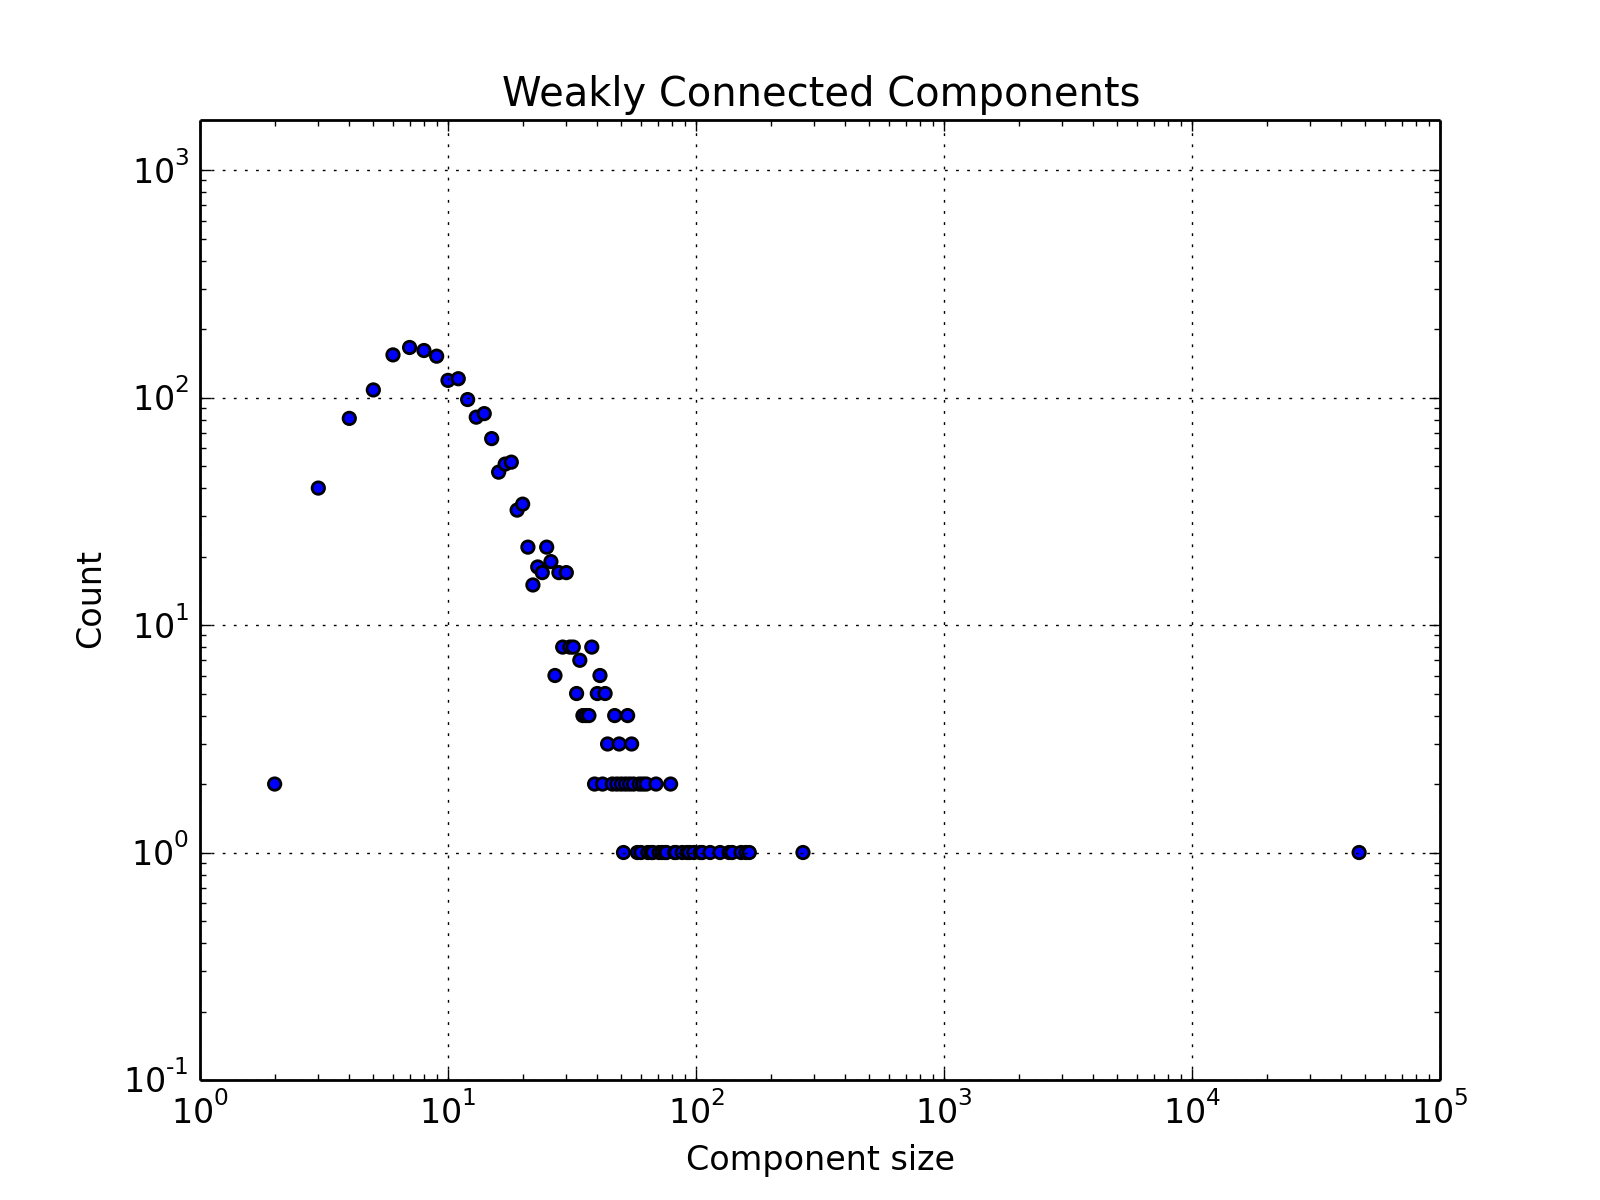
\includegraphics[width=0.35\textwidth]{FIG/plotConncompoutput_com-amazon.png} 
     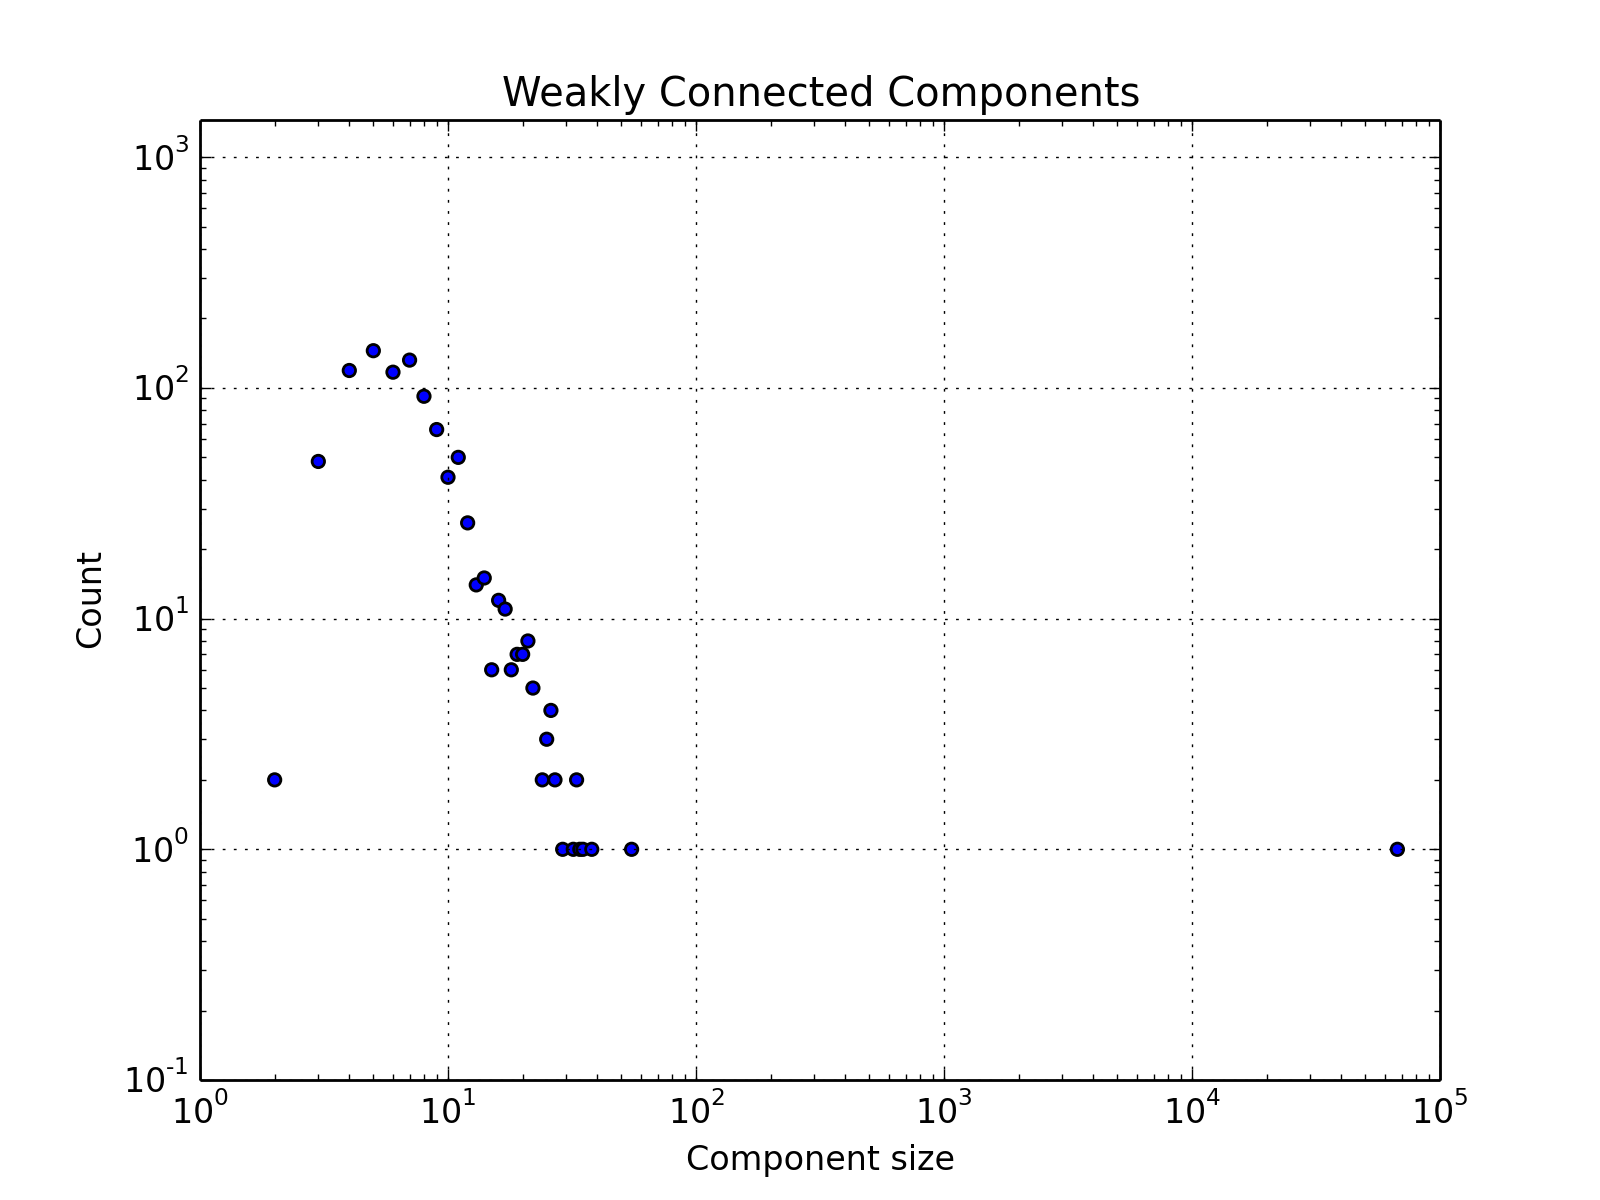
\includegraphics[width=0.35\textwidth]{FIG/plotConncompoutput_com-dblp.png} \\
     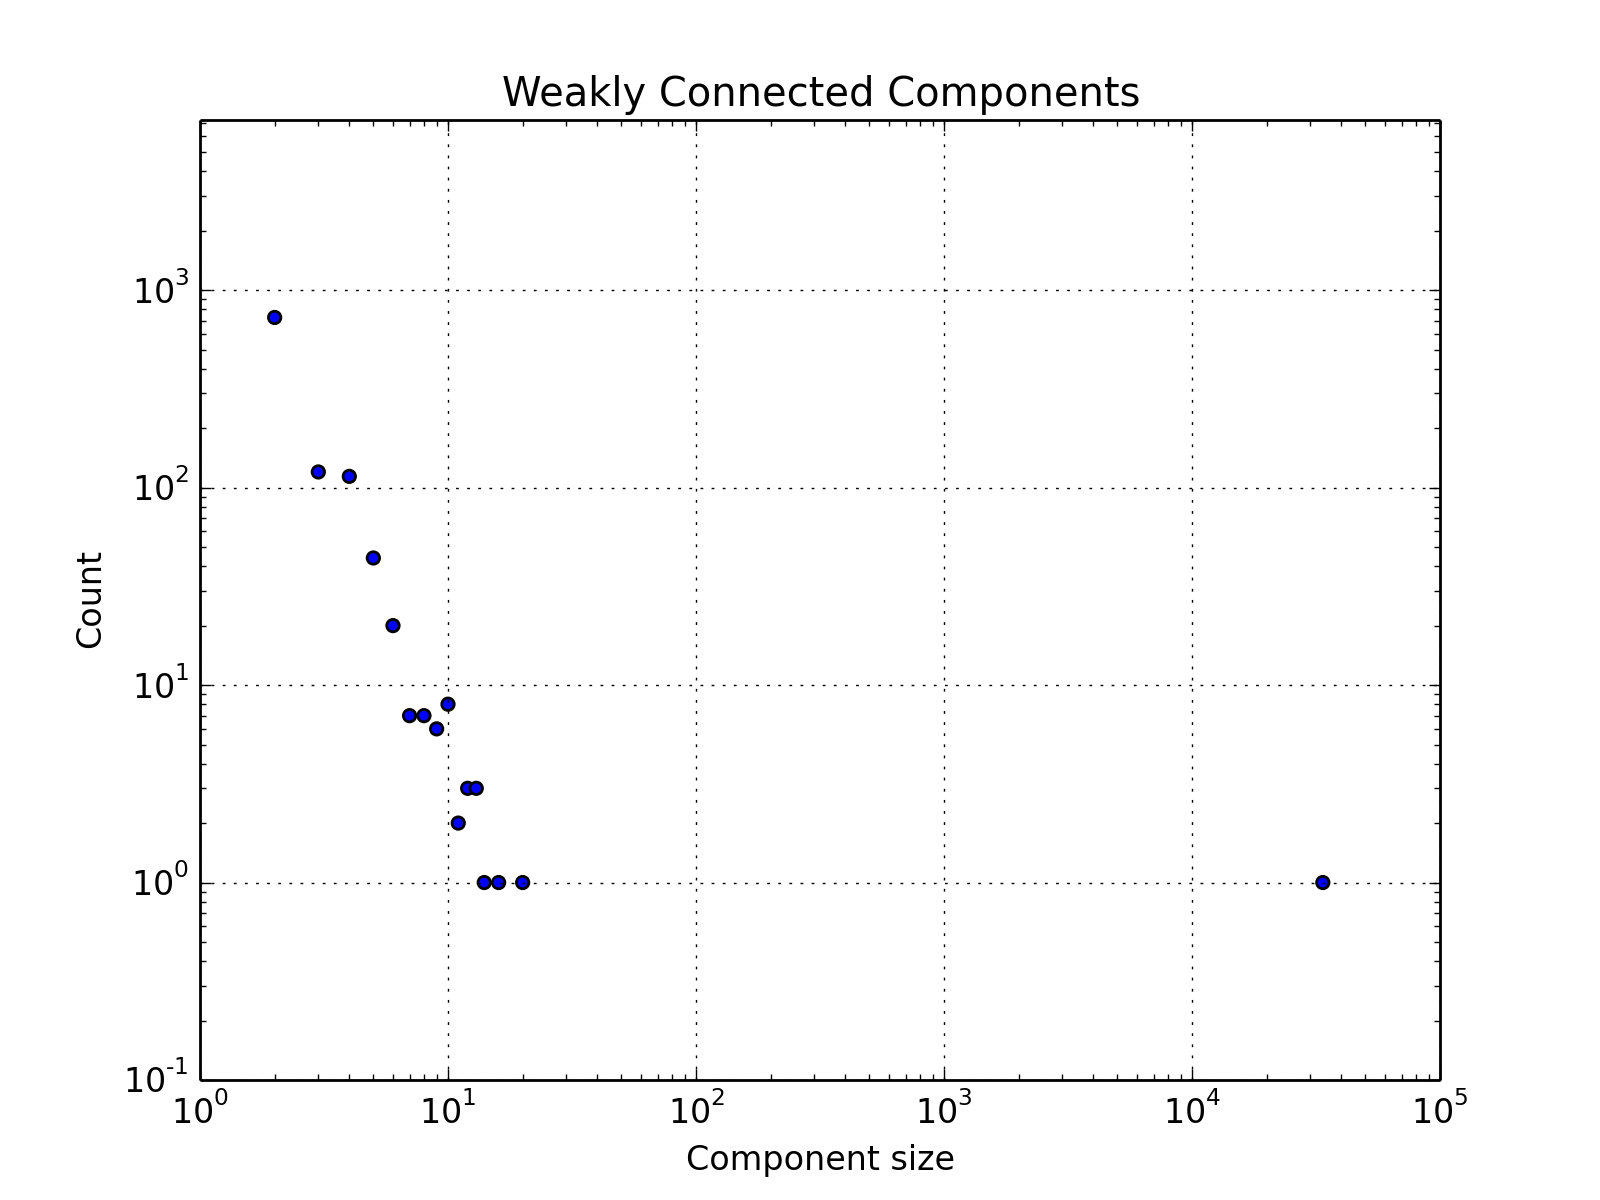
\includegraphics[width=0.35\textwidth]{FIG/plotConncompoutput_email-Enron.png} 
     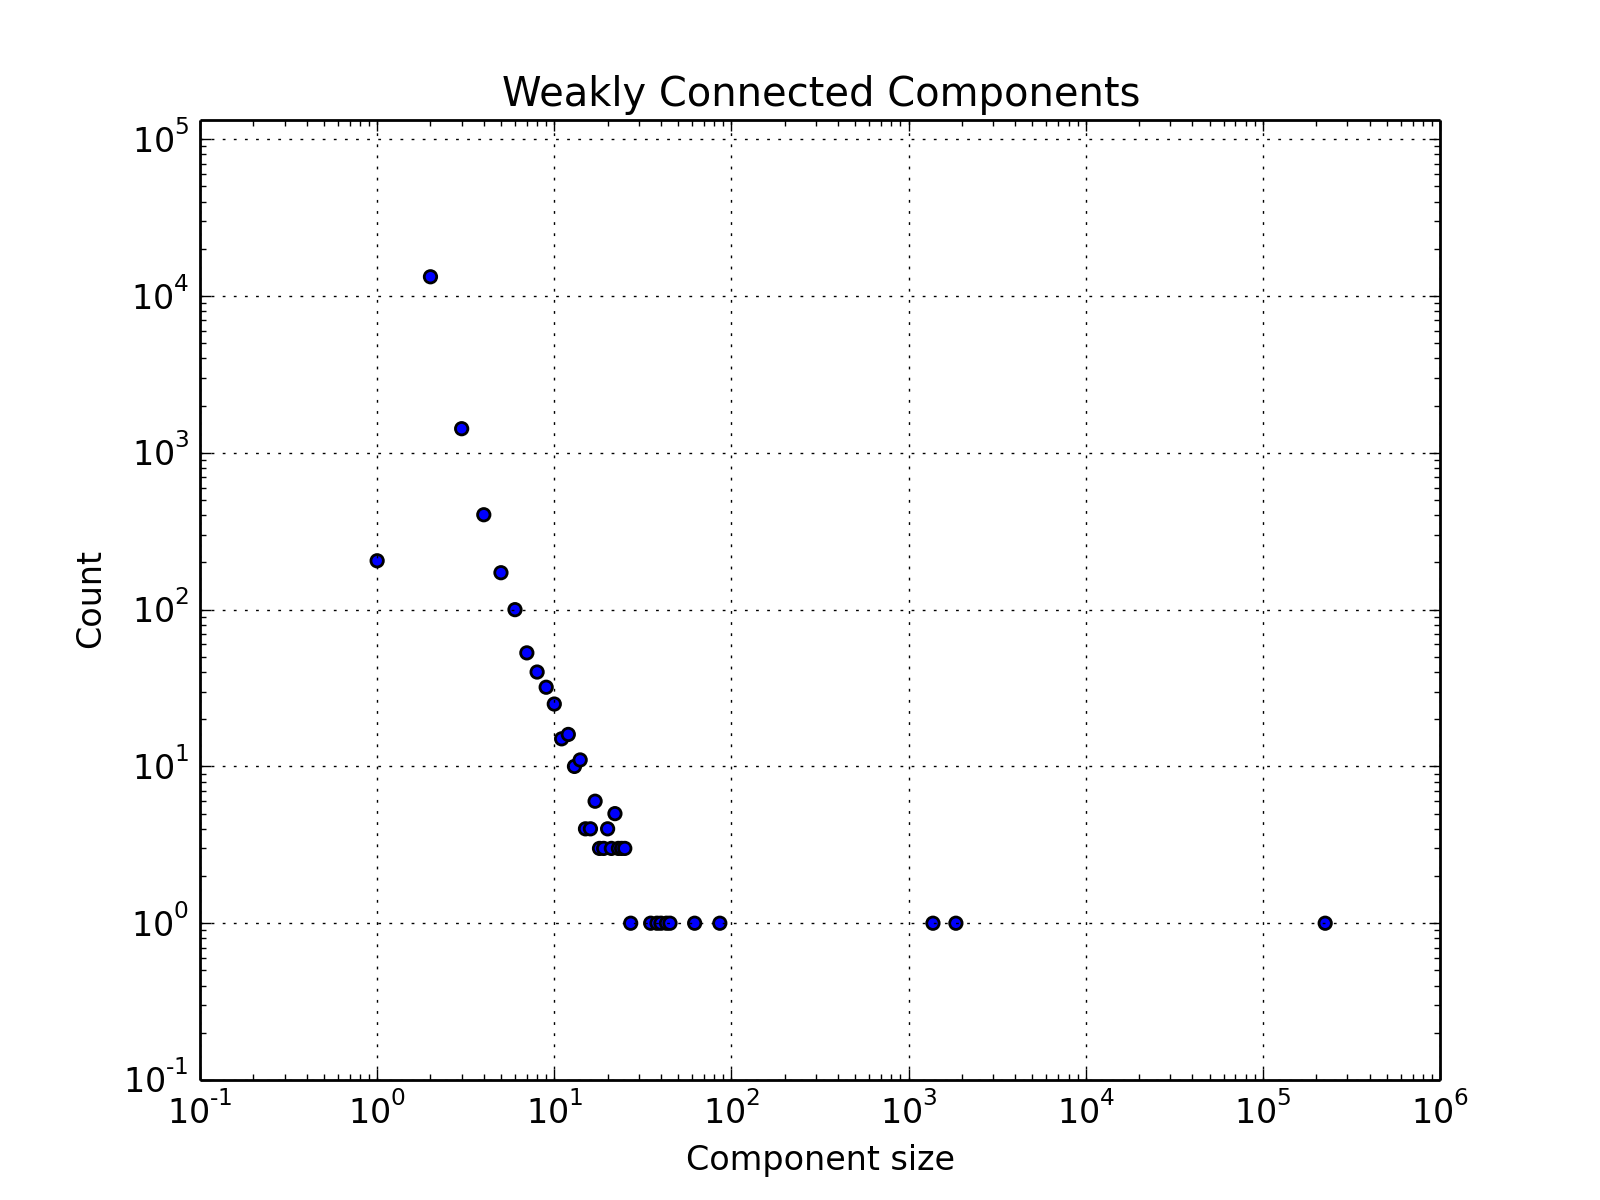
\includegraphics[width=0.35\textwidth]{FIG/plotConncompoutput_email-EuAll.png} 
     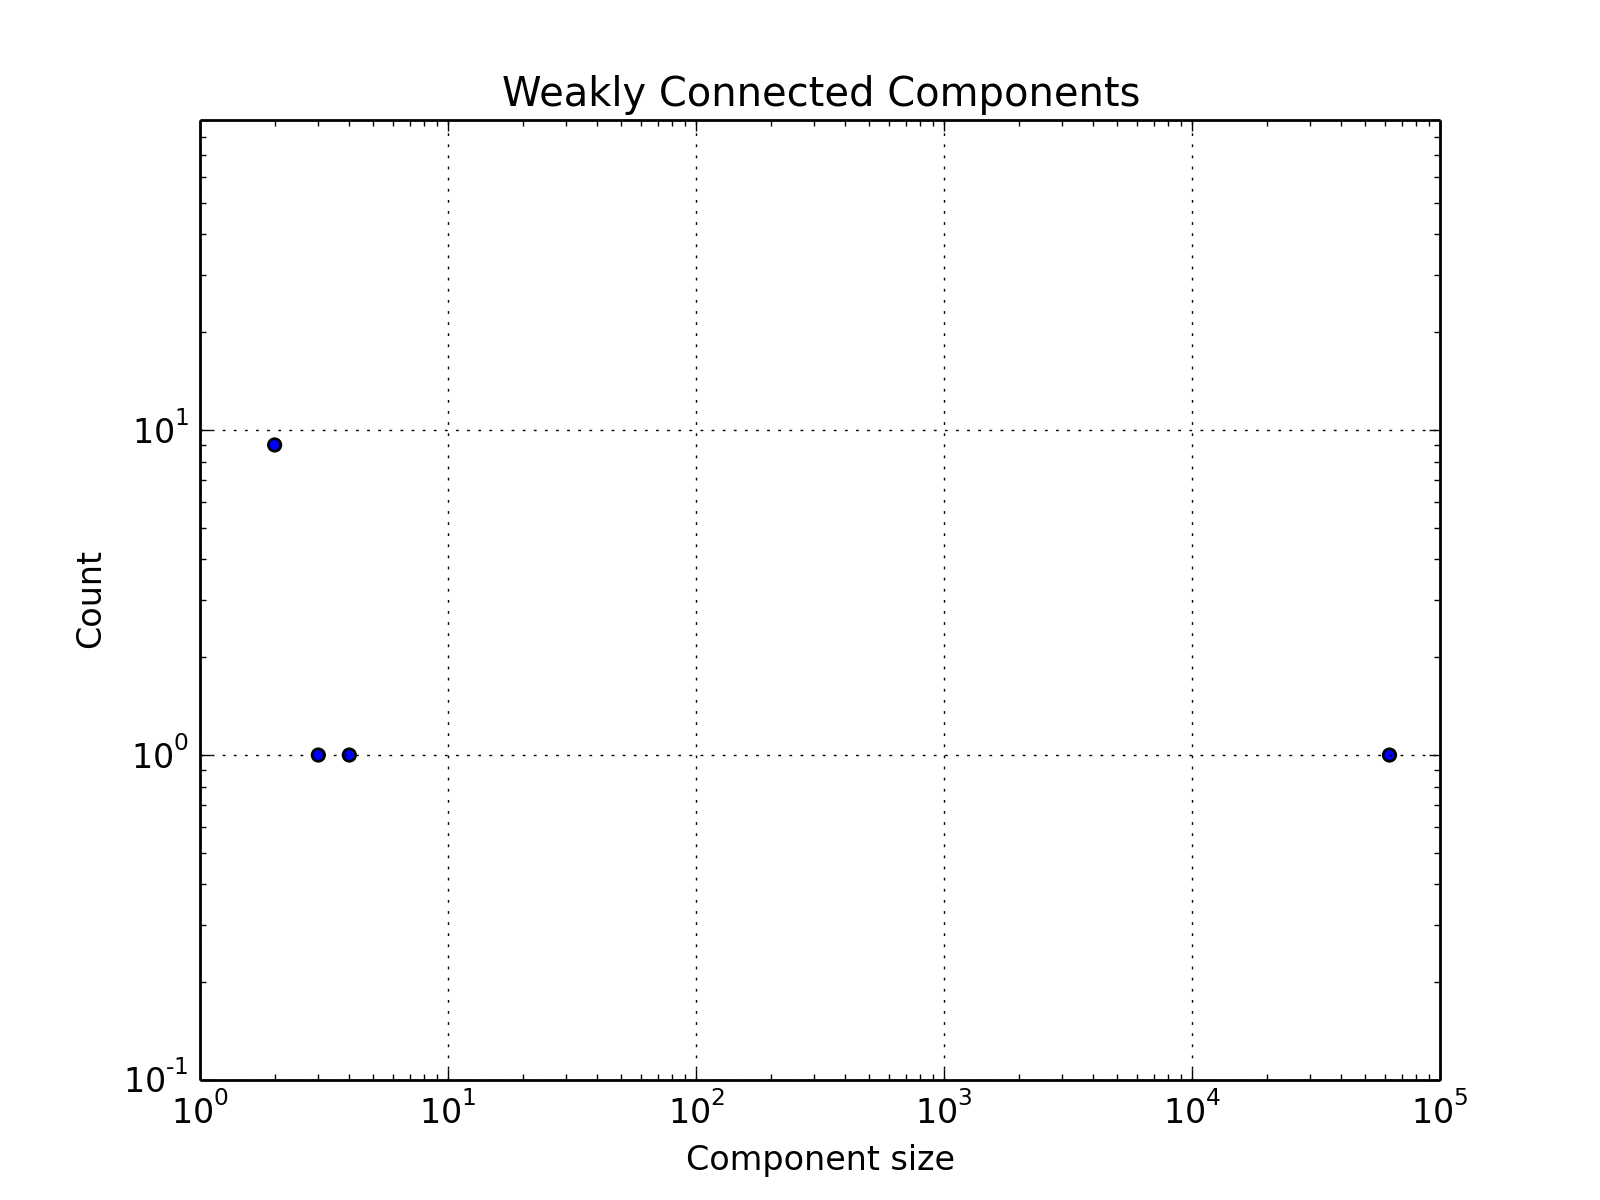
\includegraphics[width=0.35\textwidth]{FIG/plotConncompoutput_p2p-Gnutella31.png} \\
     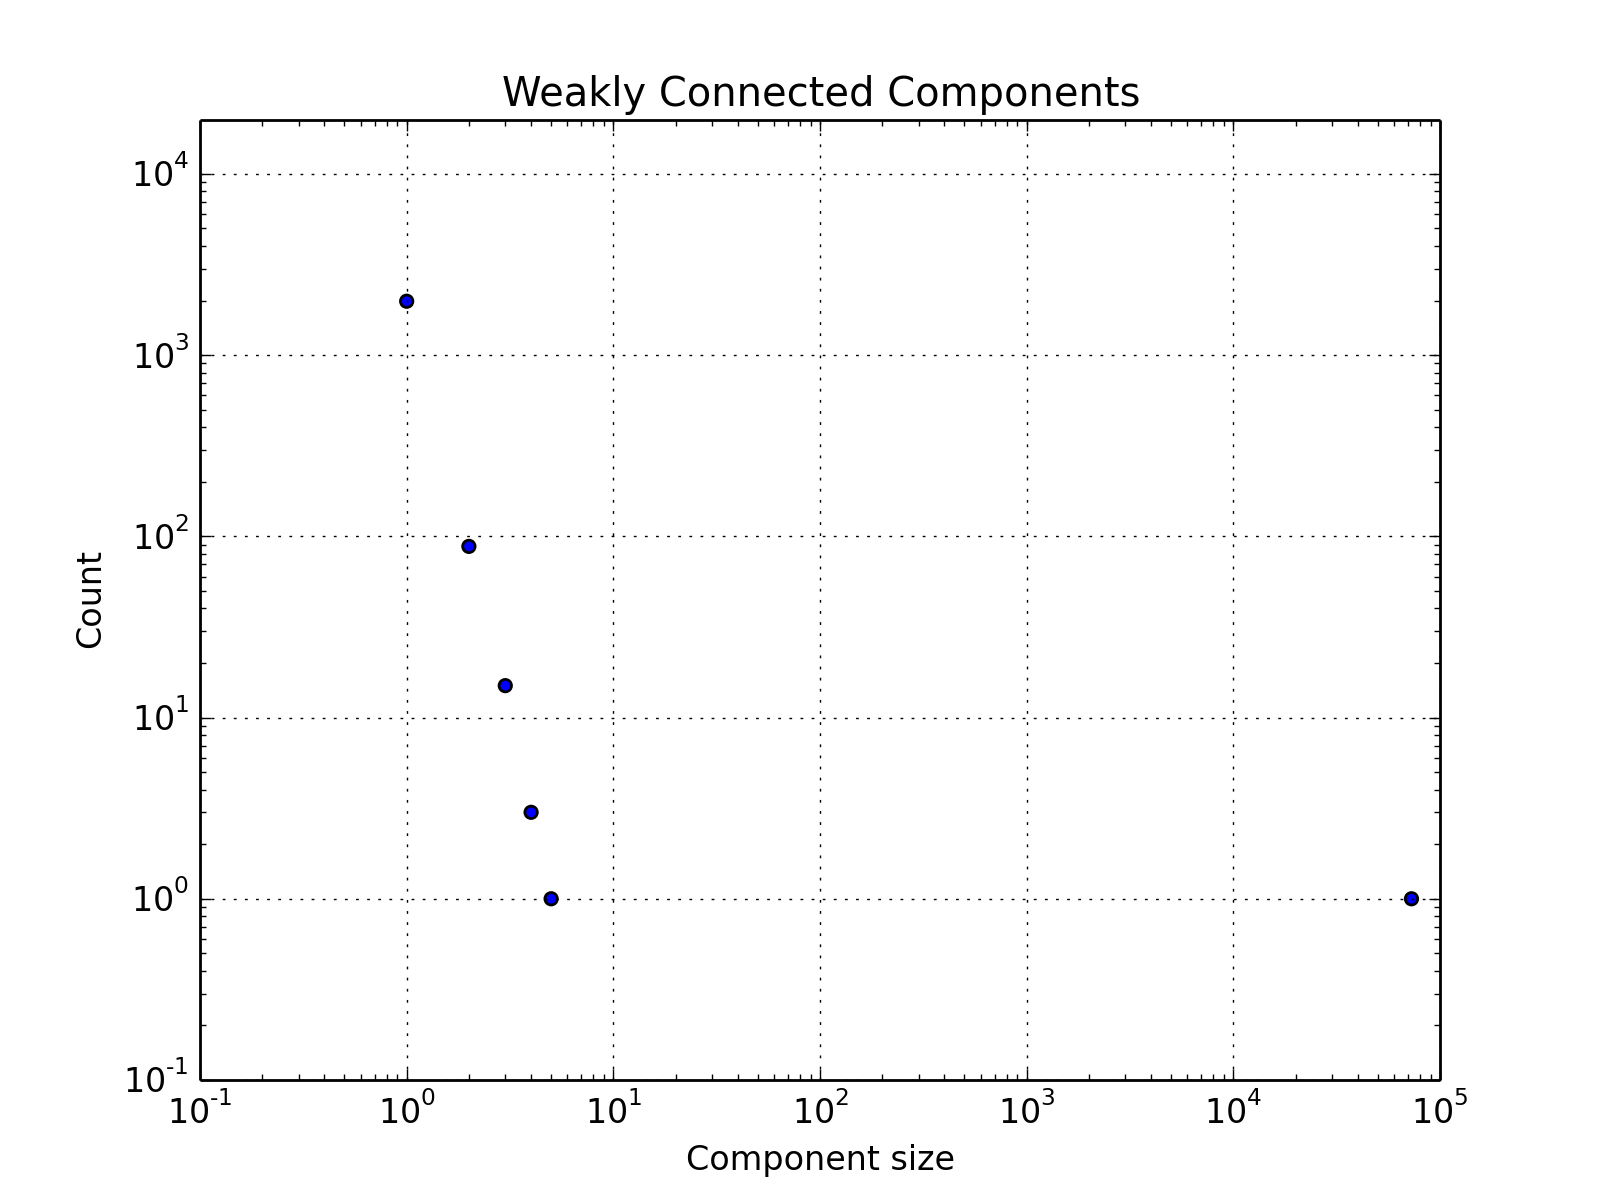
\includegraphics[width=0.35\textwidth]{FIG/plotConncompoutput_soc-Slashdot0811-75000.png} 
\end{tabular}
\caption{Weakly connected components plots of 10 graphs}
\label{fig:results}
\end{center}
\end{figure}

\textbf{Observation:}
\par Connected components of size 1 are essentially isolated points on the edge of the graph, the number of such components is generally small, as shown in the plots. Starting from size 2, the component size and corresponding count generally obeys the power law.

\subsection{Radius}

\begin{figure}[H]
\begin{center}
\begin{tabular}{ccc}
     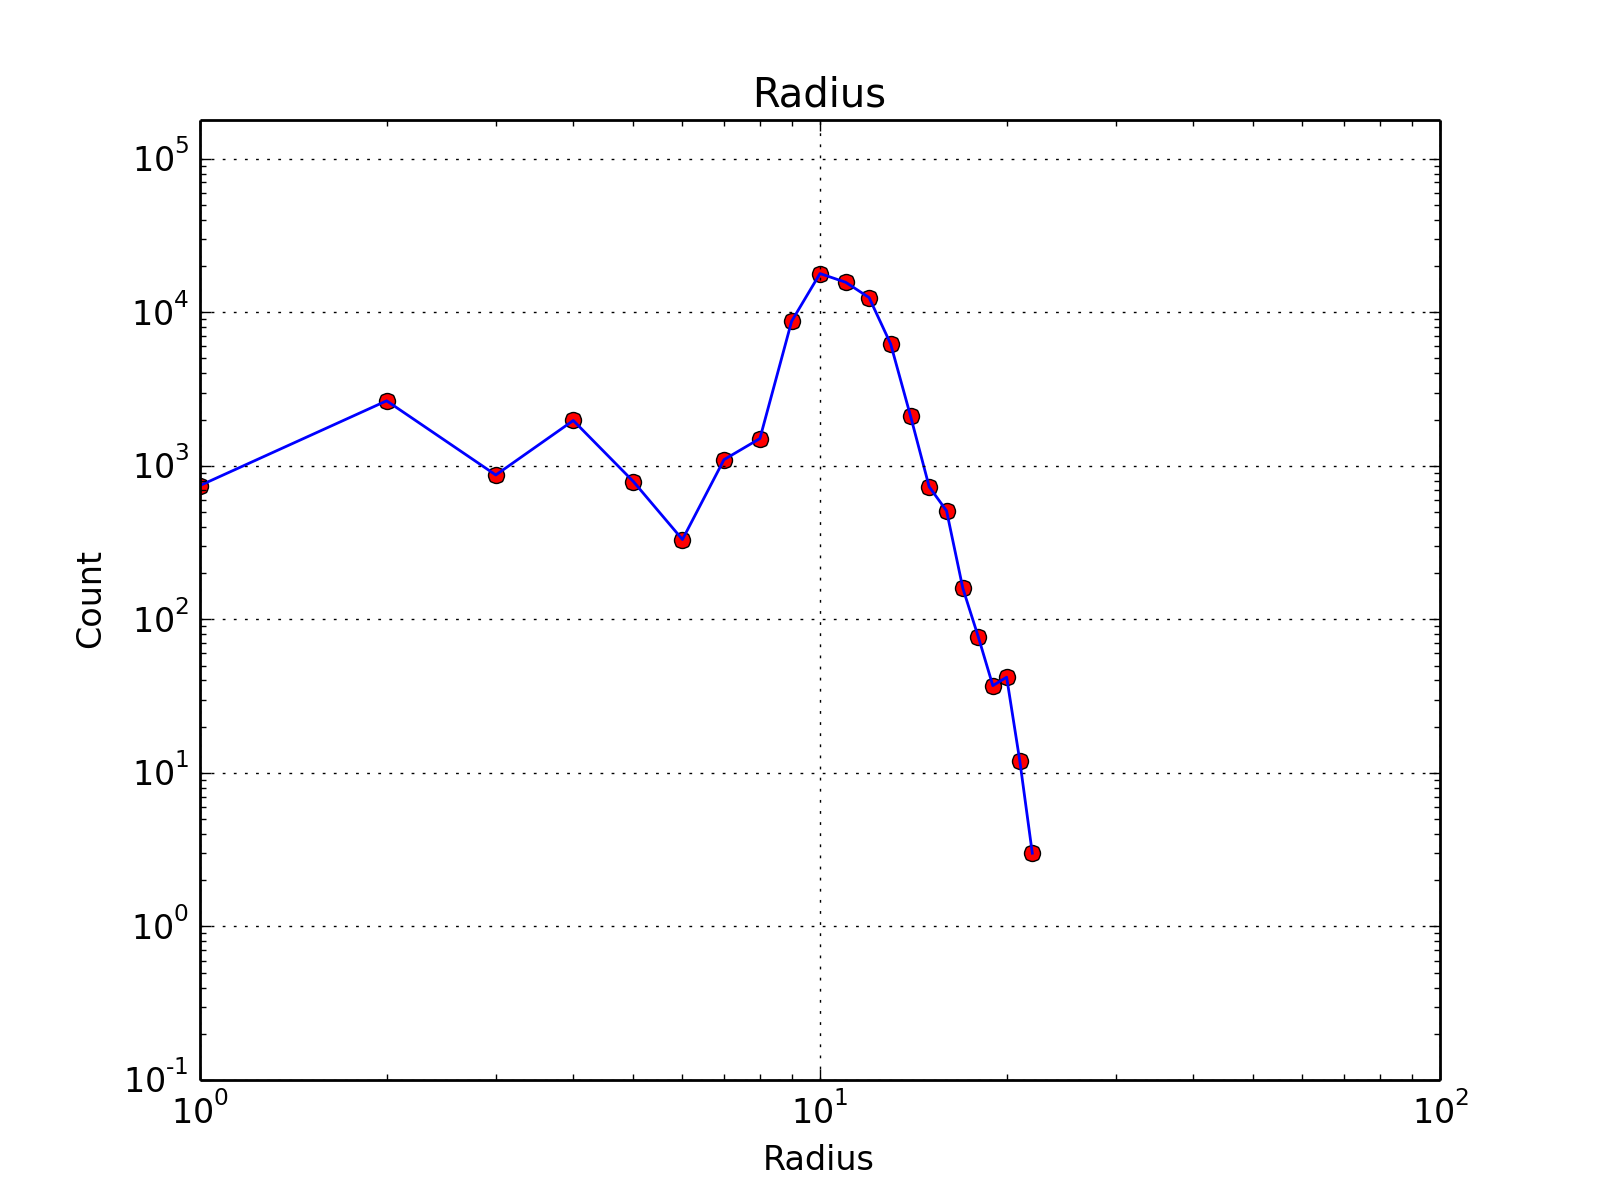
\includegraphics[width=0.35\textwidth]{FIG/Radiusoutput_as-skitter.png} 
     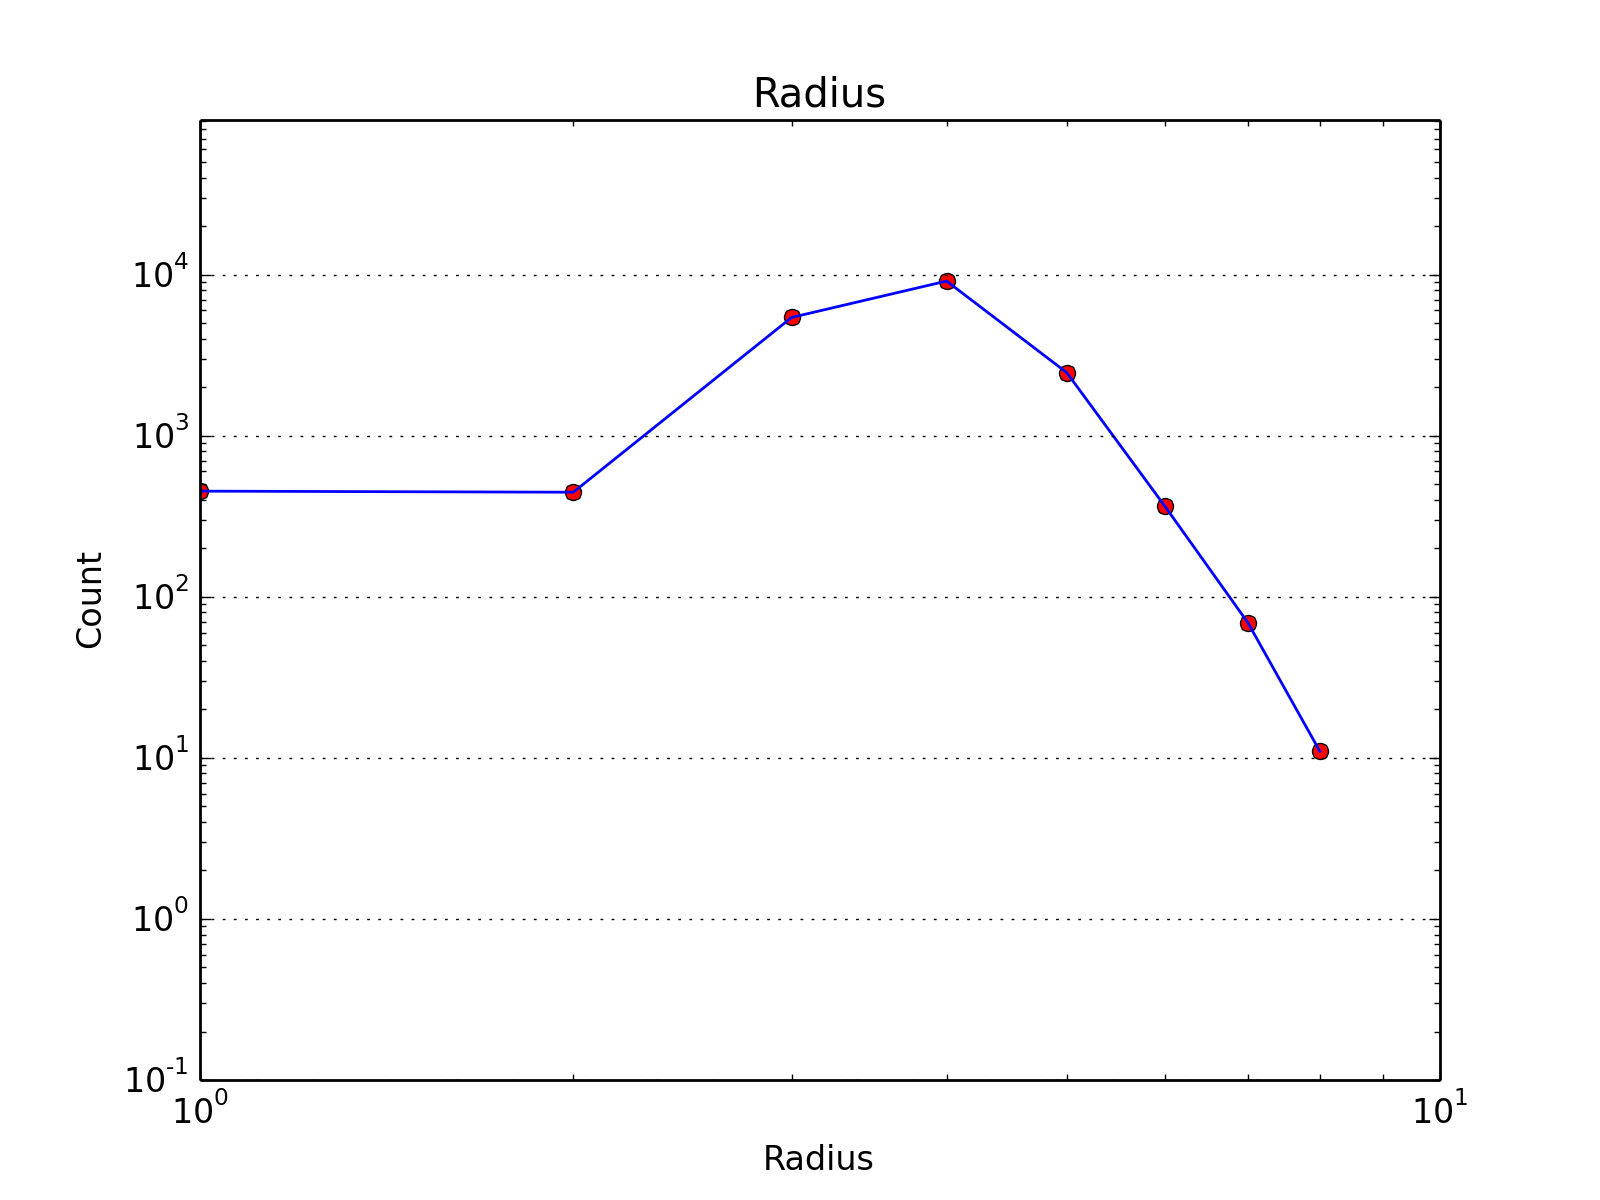
\includegraphics[width=0.35\textwidth]{FIG/Radiusoutput_ca-AstroPh.png}
     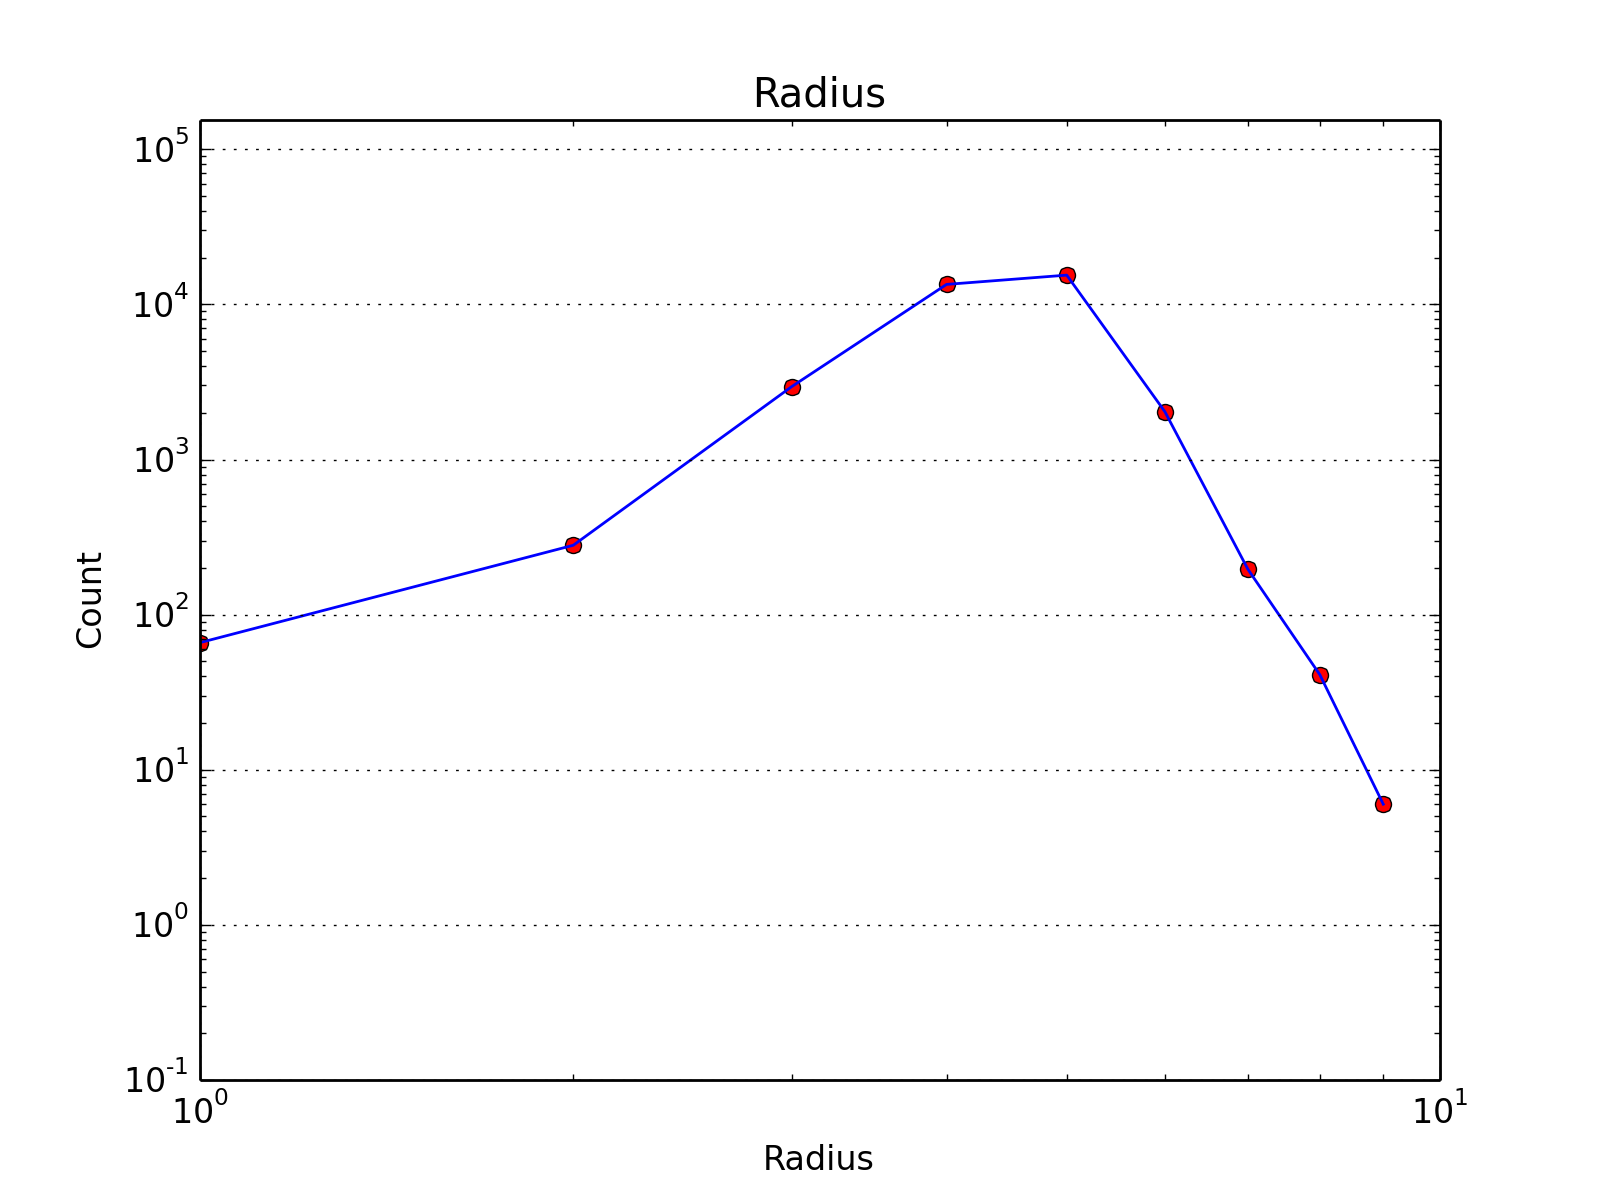
\includegraphics[width=0.35\textwidth]{FIG/Radiusoutput_cit-HepPh.png} \\
     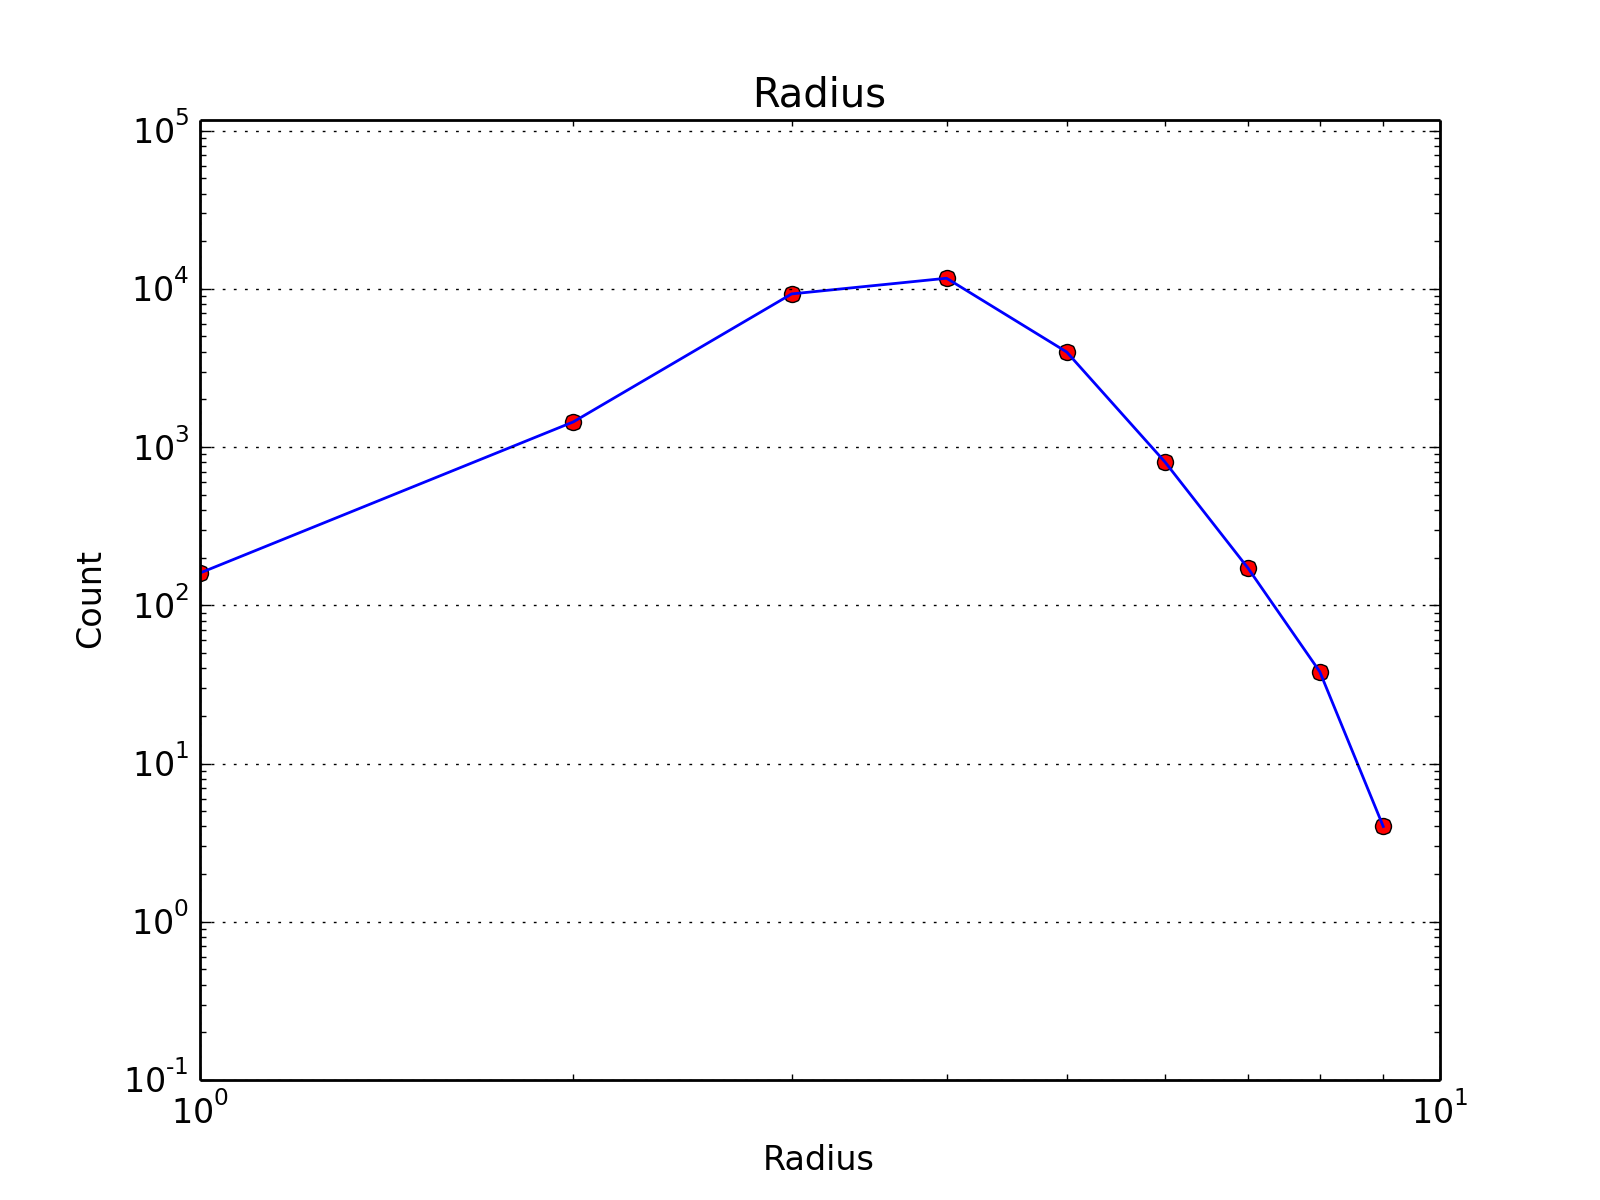
\includegraphics[width=0.35\textwidth]{FIG/Radiusoutput_cit-HepTh.png} 
     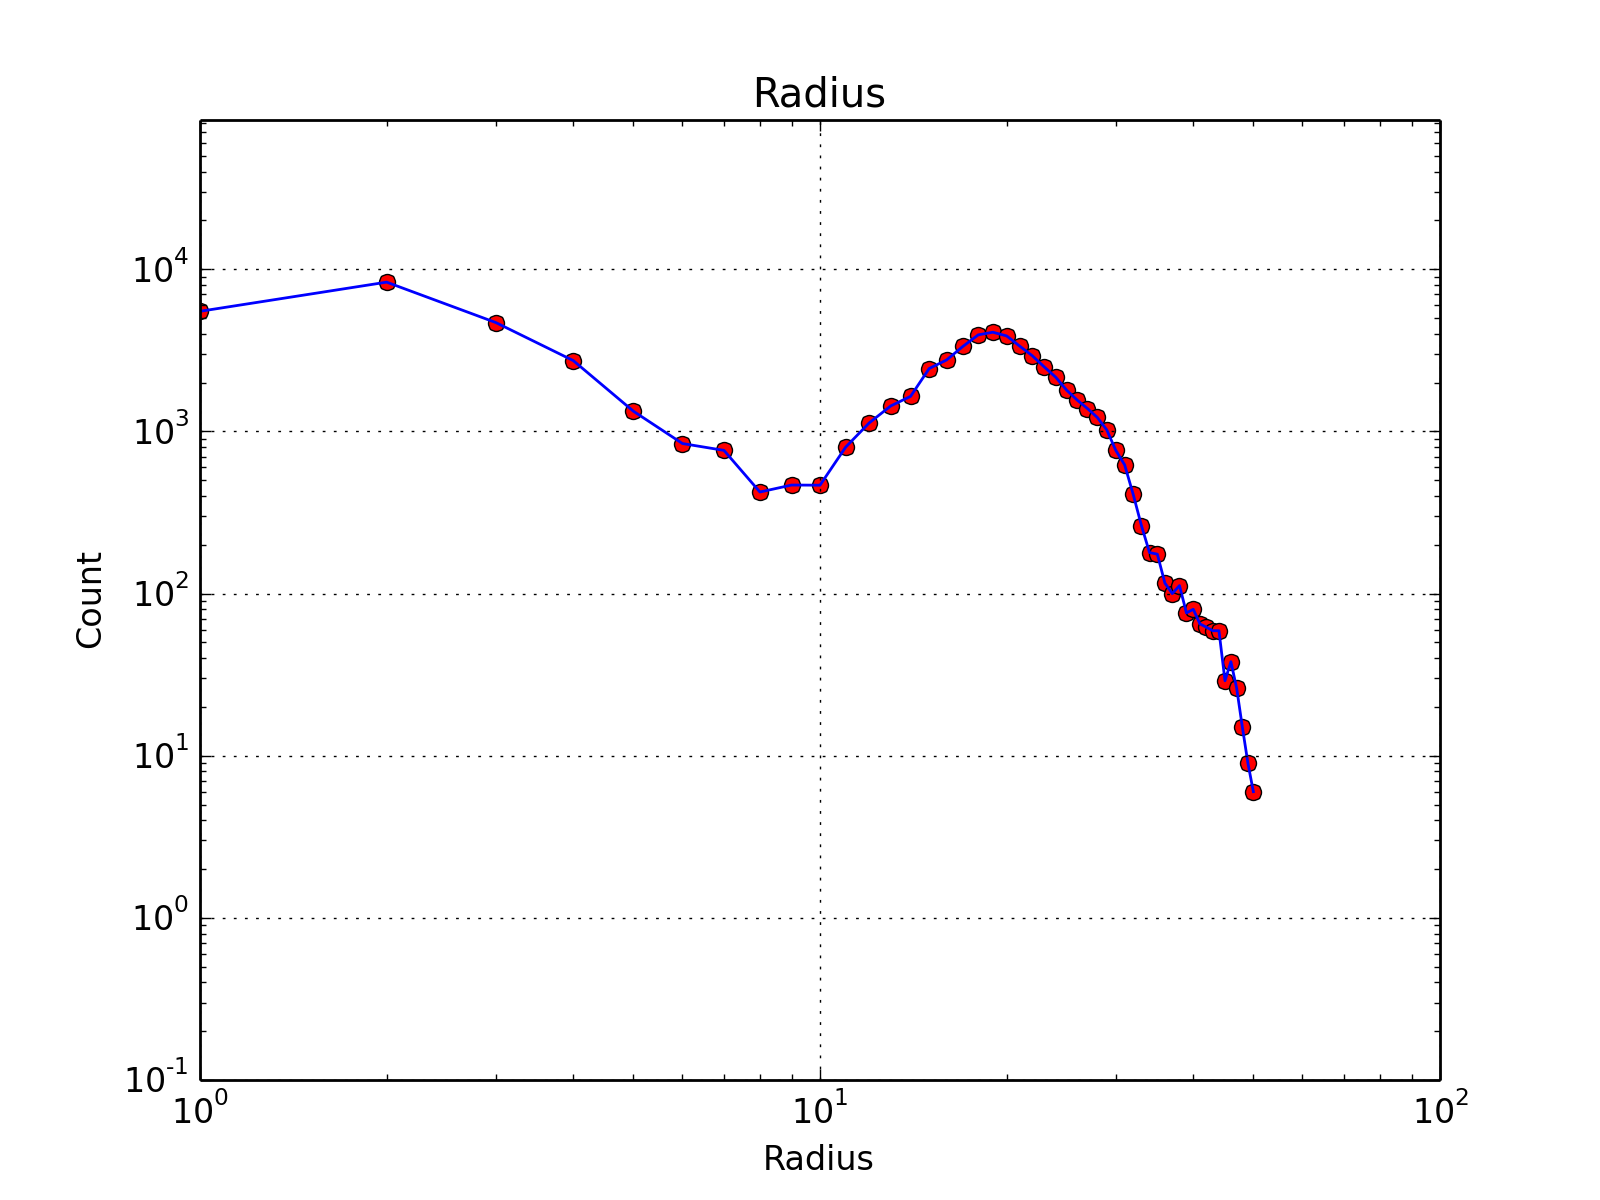
\includegraphics[width=0.35\textwidth]{FIG/Radiusoutput_com-amazon.png} 
     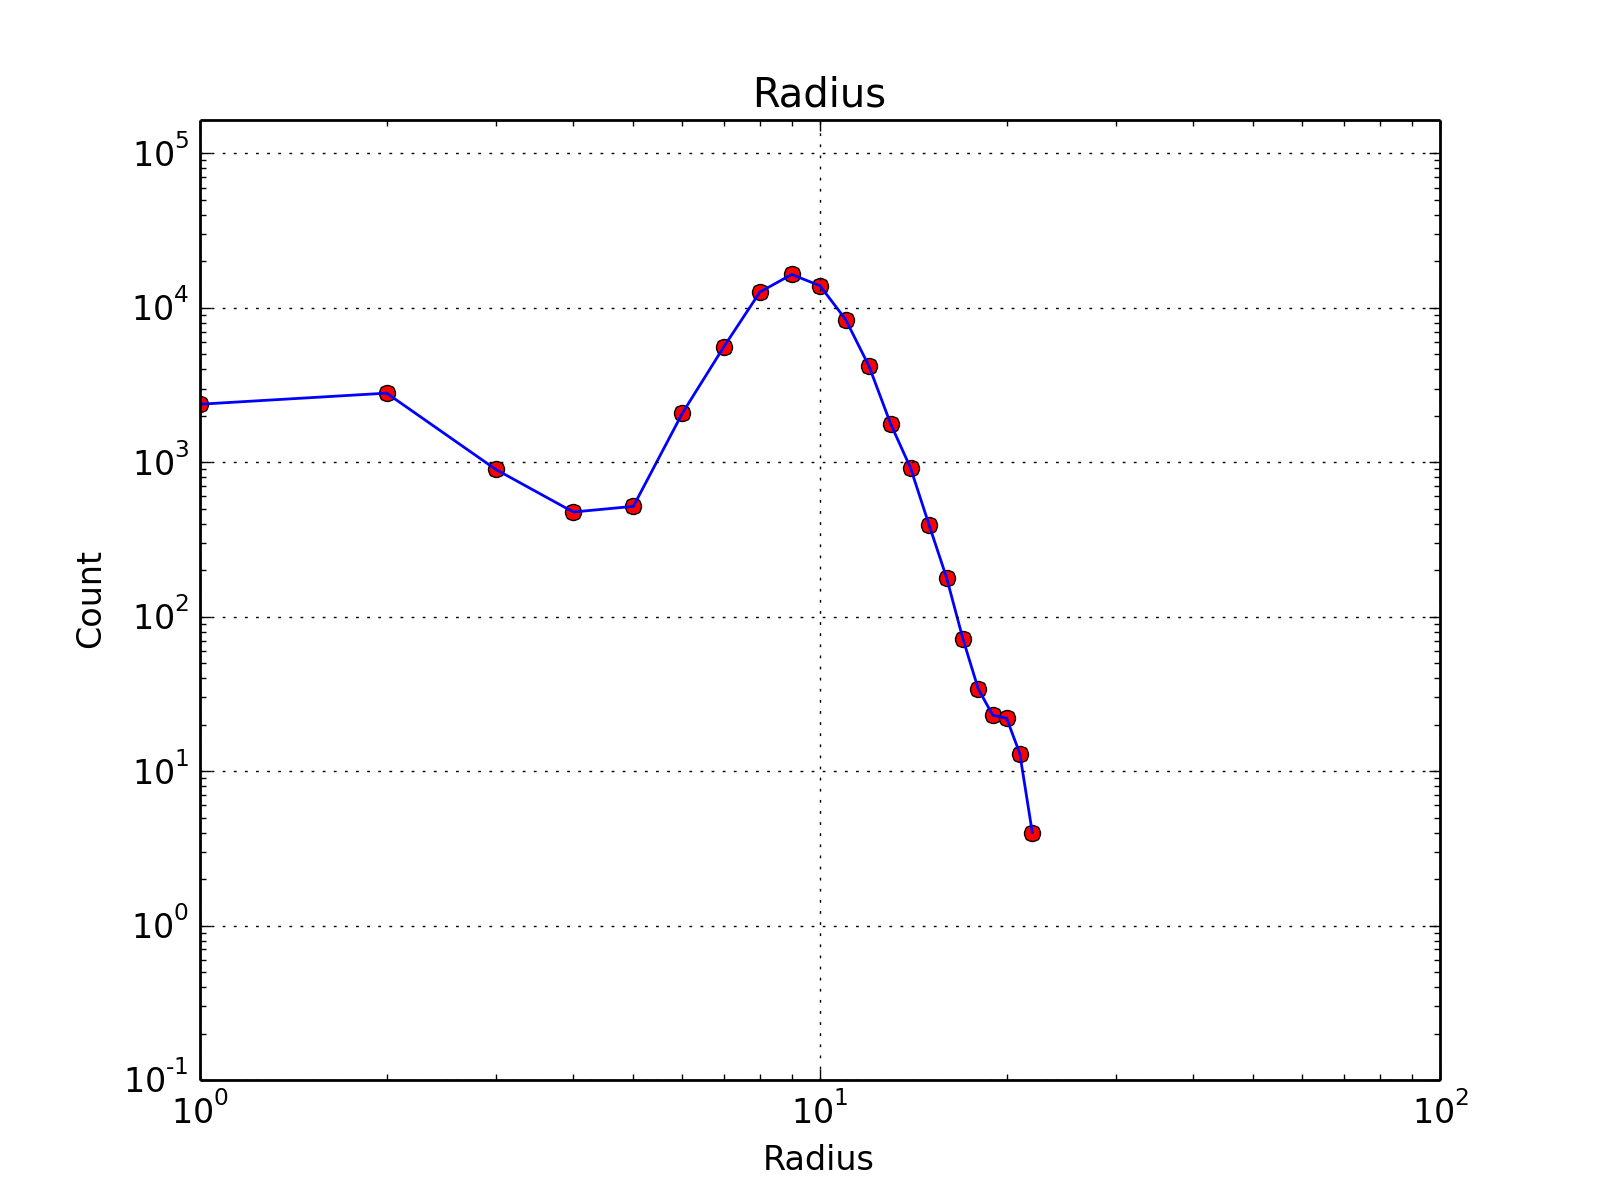
\includegraphics[width=0.35\textwidth]{FIG/Radiusoutput_com-dblp.png} \\
     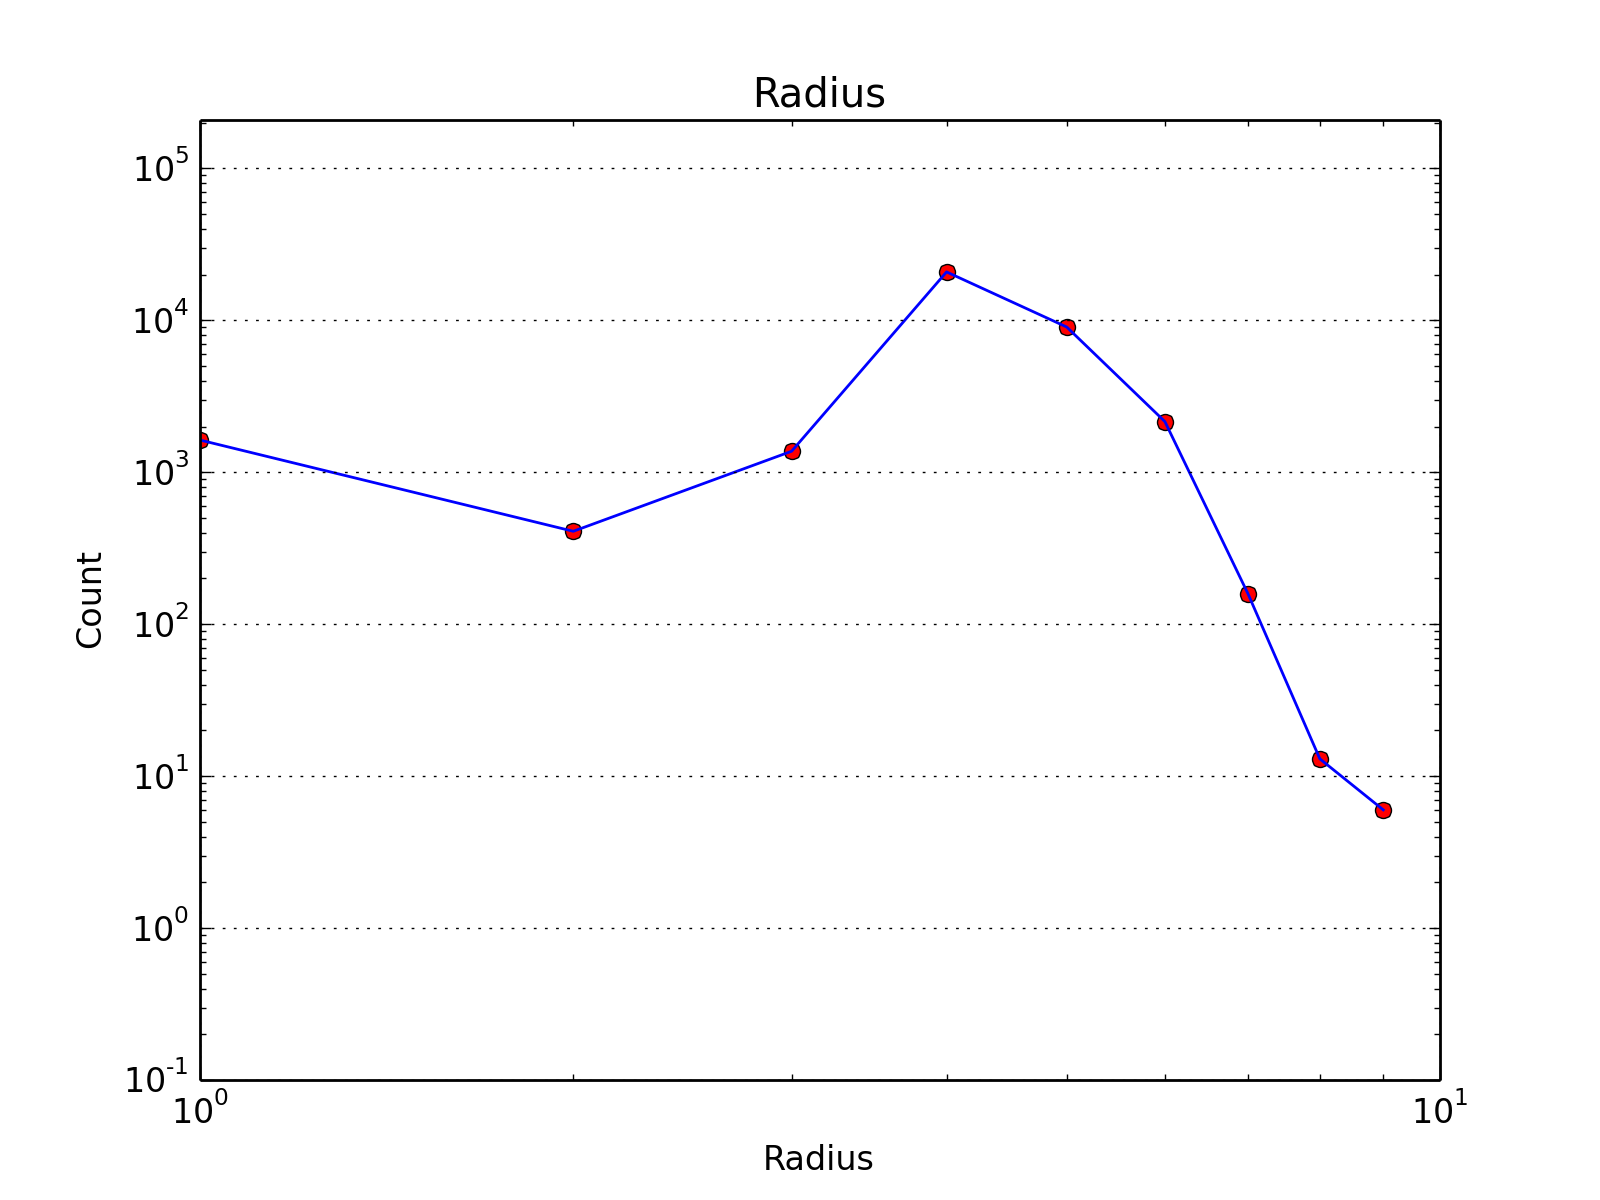
\includegraphics[width=0.35\textwidth]{FIG/Radiusoutput_email-Enron.png} 
     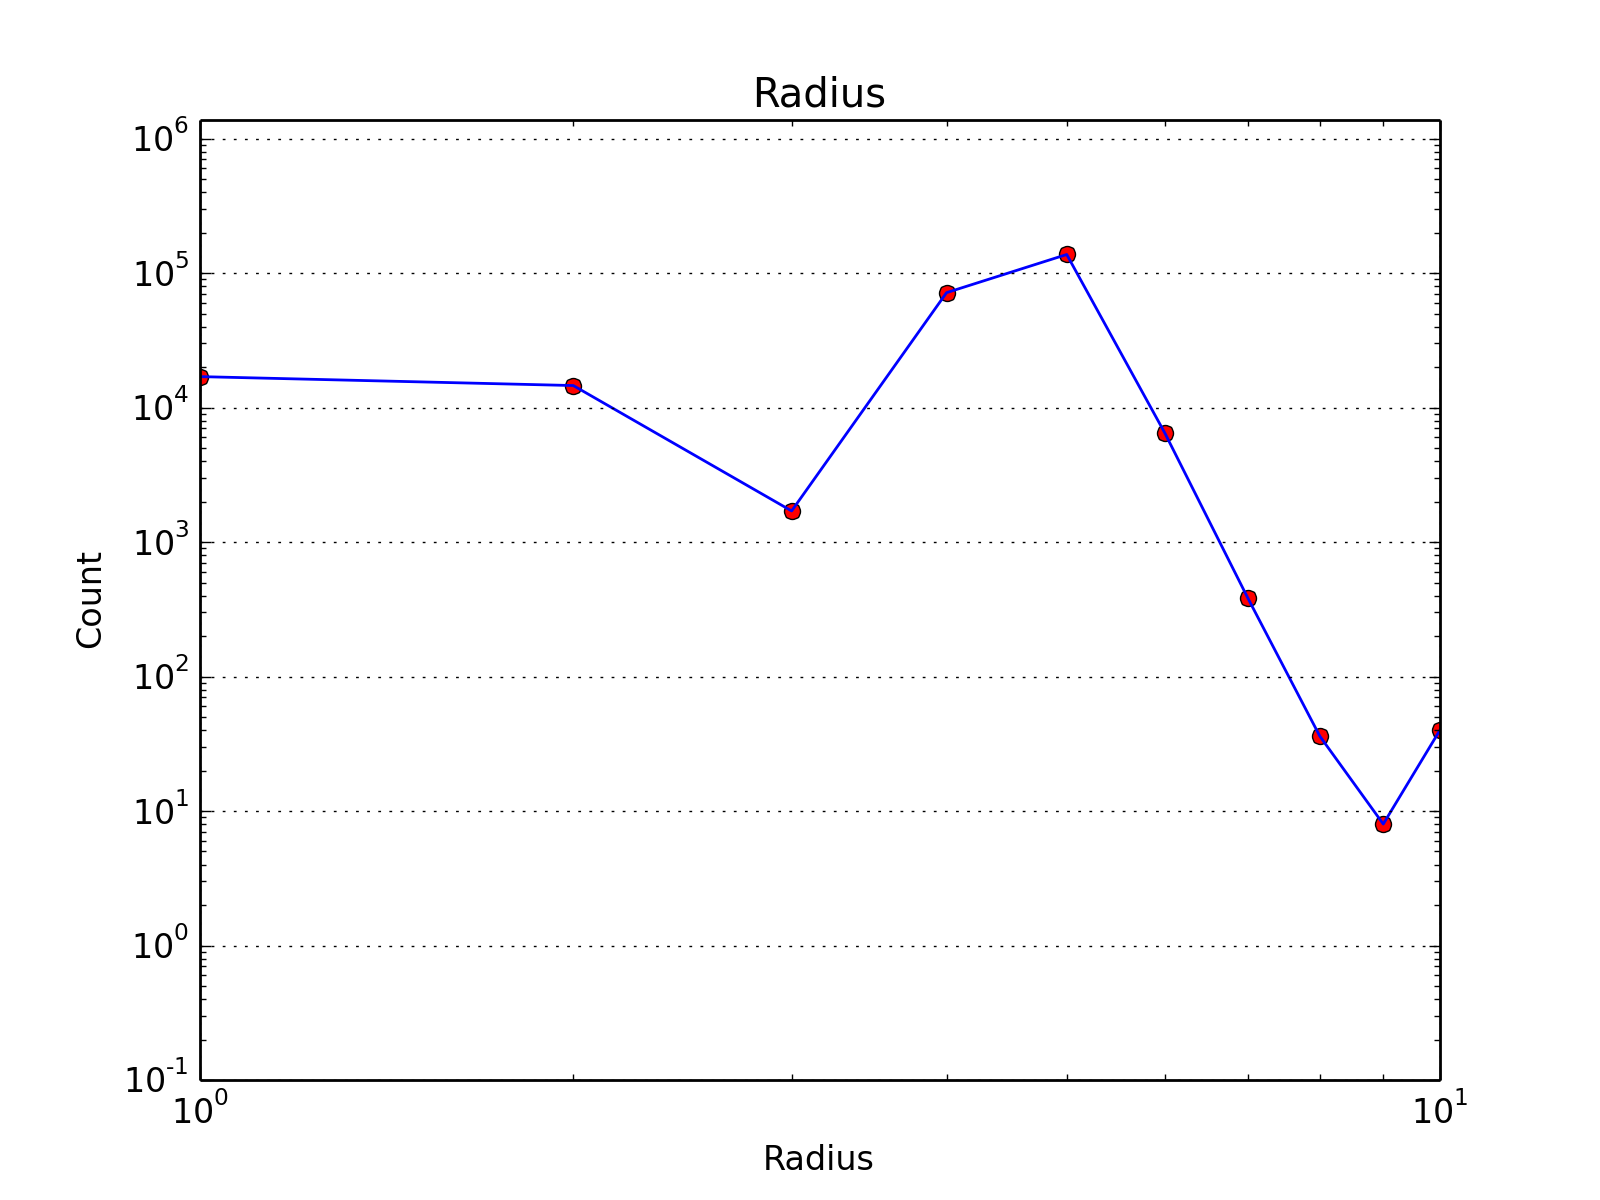
\includegraphics[width=0.35\textwidth]{FIG/Radiusoutput_email-EuAll.png} 
     \includegraphics[width=0.35\textwidth]{FIG/Radiusoutput_p2p-Gnutella31.png} \\
     \includegraphics[width=0.35\textwidth]{FIG/Radiusoutput_soc-Slashdot0811-75000.png} 
\end{tabular}
\caption{Radius plots of 10 graphs}
\label{fig:results}
\end{center}
\end{figure}

\textbf{Observation:}
\par Most Radius vs. Count plot has one distinct peak.

\subsection{KCore}

\begin{figure}[H]
\begin{center}
\begin{tabular}{ccc}
     \includegraphics[width=0.35\textwidth]{FIG/plotKcoreoutput_as-skitter.png} 
     \includegraphics[width=0.35\textwidth]{FIG/plotKcoreoutput_ca-AstroPh.png}
     \includegraphics[width=0.35\textwidth]{FIG/plotKcoreoutput_cit-HepPh.png} \\
     \includegraphics[width=0.35\textwidth]{FIG/plotKcoreoutput_cit-HepTh.png} 
     \includegraphics[width=0.35\textwidth]{FIG/plotKcoreoutput_com-amazon.png} 
     \includegraphics[width=0.35\textwidth]{FIG/plotKcoreoutput_com-dblp.png} \\
     \includegraphics[width=0.35\textwidth]{FIG/plotKcoreoutput_email-Enron.png} 
     \includegraphics[width=0.35\textwidth]{FIG/plotKcoreoutput_email-EuAll.png} 
     \includegraphics[width=0.35\textwidth]{FIG/plotKcoreoutput_p2p-Gnutella31.png} \\
     \includegraphics[width=0.35\textwidth]{FIG/plotKcoreoutput_soc-Slashdot0811-75000.png} 
\end{tabular}
\caption{KCore plots of 10 graphs}
\label{fig:results}
\end{center}
\end{figure}

\textbf{Observation:}
\par Some graphs show power law on the component size vs. count, e.g, graph No.4 and No.5.